%\chapter{Histological grade prediction via automatic liver tumors segmentation}\label{contributions_xp}


%In this chapter we present the experimental results of our work.
%We first describe more precisely the different key concepts 
%to be implemented such as the cascaded architecture or the 
%incorporation of the multiphase images.
%We then expose our semantic segmentation experiments where 
%the best performances were obtained by stacking several 
%specialized networks with dynamic contrast-enhanced images as input.
%After validating the value brought by our semantic segmentation architecture
%to provide additional annotations in the case of weakly annotated datasets, 
%we describe our \ac{dlr} pipeline which incorporates the relevant semantic imaging features 
%for the prediction of the histological grade.

\chapter{Semantic segmentation applied to the study of HCC}

As explained previously, state-of-the-art deep learning techniques allow
modern hardware to perform automatic segmentation of both the liver and
its structures with a precision close to the one obtained by the experts
themselves.
In this section, we will first describe the implemented
networks and the different used datasets, before presenting the experiments.
%As described previously, no real consensus was made regarding the
%design of the \ac{dl}-related semantic segmentation studies, so we decided to
%launch several experiments on selected datasets to determine the impact
%of the training strategies on the performances of the networks.
After selecting an optimal set of hyperparameters, we evaluated the
advantages brought by a cascaded architecture, and the way to implement
it, before describing the way to incorporate the multiphase information
in our architecture.
The results and the conclusions of this work were presented in the
literature \cite{Ouhmich2019}.


\section{Motivations}

We implemented different architectures to validate the hypothesis that
current deep networks can perform automatic delineation of both the
liver and its tumors. The wash-in wash-out being an important characteristic of the tumor (see chapter \ref{liverCancer}), we decided to design an architecture that will try to extract features encoding this specific information. We wanted to prove that incorporating the dynamic information through the use of contrast-enhanced images can improve the performances of the network, therefore, we compared results obtained using single and multi-phase networks. \\
We built several architectures to confirm that the cascaded approach corresponds to the best paradigm when dealing with small multiphase datasets.
Finally, we proved the ability of our cascaded architecture to provide additional annotations in weakly annotated datasets.\\
It it worth noting that we are the first to automatically 
delineate \ac{hcc} on multiphase \ac{ct} images using a \ac{dl} architecture, and that features computed by the our architecture will further be used in a radiomics purpose to predict the histological grade.



\section{Cascaded architecture}

Even though no consensus was made regarding existing methods, we noticed that
several studies implemented a sequential pipeline that can be modeled as
cascaded architecture. The cascade consists in several networks trained
to perform a specific simpler task, and that are sequentially connected, to
provide a final annotation map. In our case, the goal is the
segmentation of the liver and its internal structures with the
differentiation between parenchyma, and both the active and the necrotic
parts of the hepatic tumor.
Our cascade will consequently be composed of 3 networks, as depicted
in the figure \ref{CARS_Cascade}. The first one will be specialized to segment the liver in
abdominal axial slices, the second will delineate the contours of the
tumor in the predicted liver \ac{roi}, whereas the final one will
differentiate between active and necrotic parts within the obtained
tumor \ac{roi} \cite{Ouhmich2019}.
Each one of the given networks will share the same \emph{U-Net}
architecture.

\begin{figure}[th!]
	\centering
	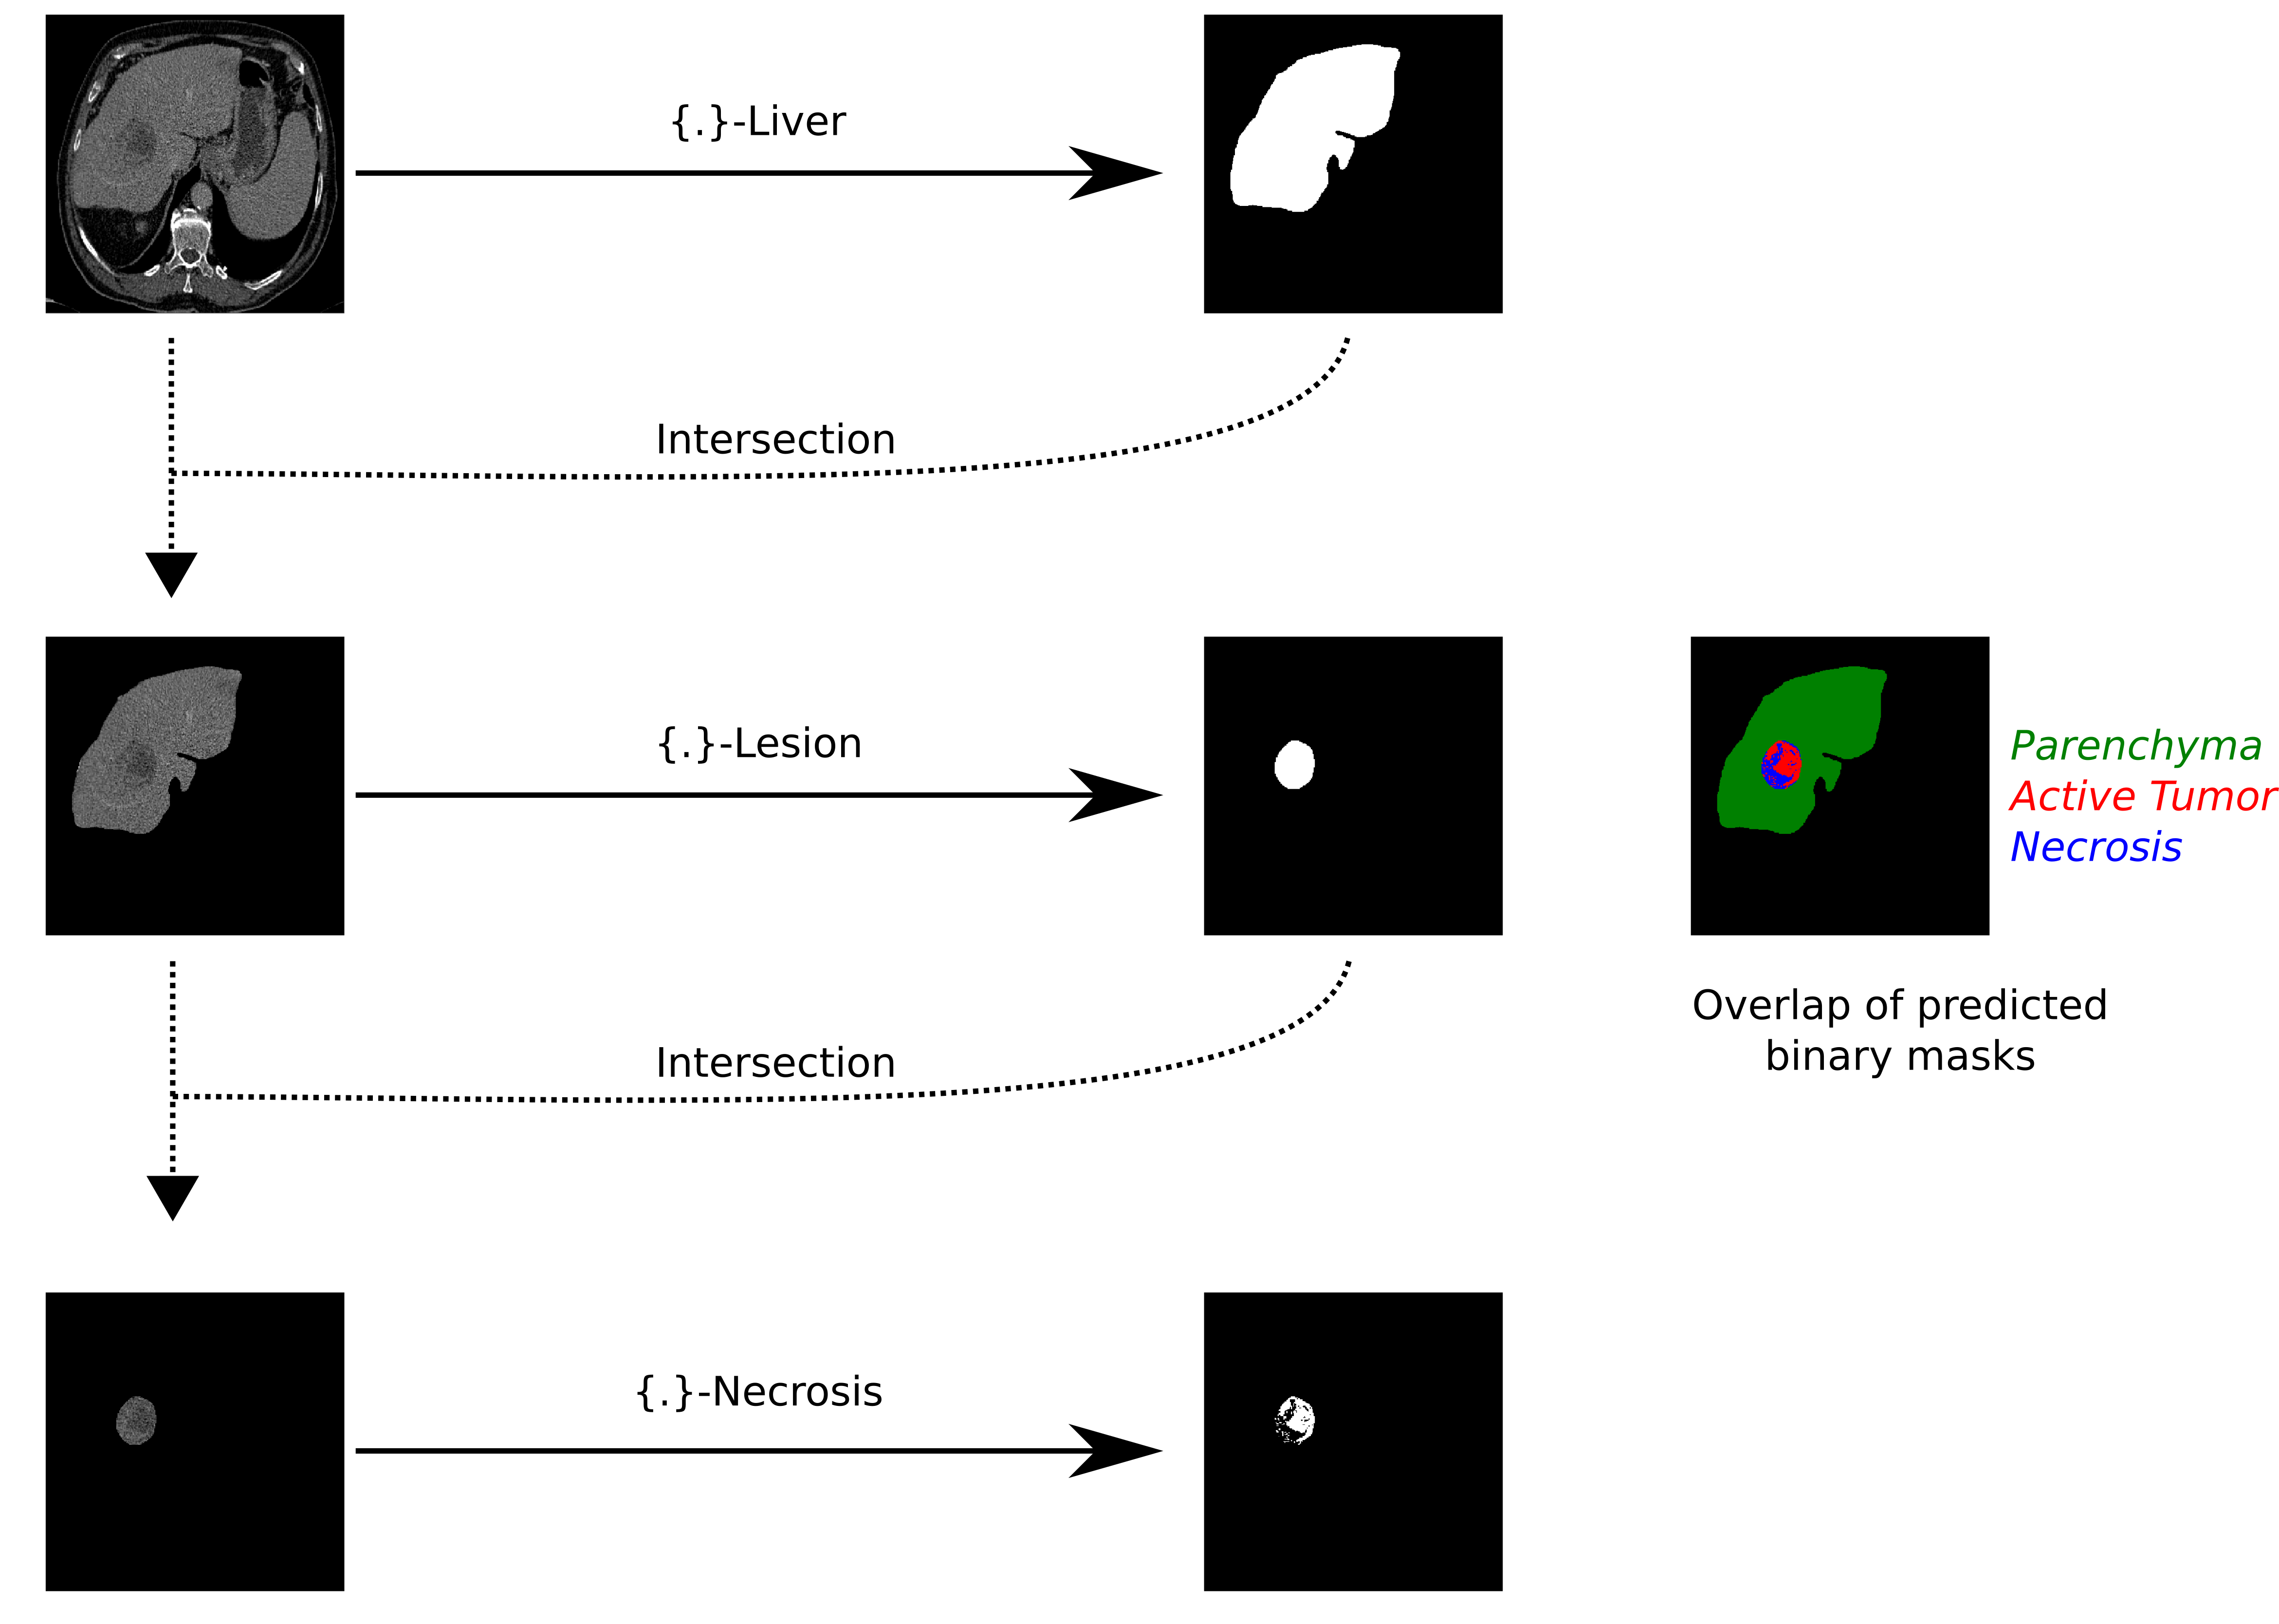
\includegraphics[width=0.7\linewidth]{../SemanticSeg/images/Cascade2}
	\caption{Cascaded network: The first network takes as input a \ac{ct} image and segments the liver. The resulting segmentation map is used to remove non-liver pixels in the input data of the second network which performs the segmentation of lesions. The last network segments the necrosis within the lesions. The three binary masks are combined in the final segmentation map.}
	\label{CARS_Cascade}
\end{figure}


\section{U-Net network}

As a basis architecture, we have decided to implement \emph{U-Net} like
networks because it has been previously used for the semantic
segmentation task, and has proven to give good results even with a
small number of training samples. \\
The original \emph{U-Net} architecture was developed by Ronneberger et
al. \cite{Ronneberger2015} and initially designed for the
delineation of cells in microscopic images. As detailed previously, the
network can be divided into two subparts, a contraction one where the
information contained within the images is compressed, through the
extraction of high to low level features, and a decoding part where the
compressed information is used to reconstruct a high resolution
segmentation. The architecture was initially composed of 19
convolutional layers, with a rectified linear unit function as
activation. The input image had an initial size of $ 512\times512 $ pixels, and
at each stage of the encoding part, 2 convolutional layers are stacked
with an increased number of filters. The initial pair of convolution
layers used 64 filters each, whereas the final stage of the encoding
stage used 1024 filters. After each pair of convolutional layers, a max
pooling layer is applied to halve the spatial dimension of the features
maps. As a result, a $ 30\times30\times1024 $ features map is produced at the
bottleneck of the network. This representation is then reformatted in
the decoding part to obtain a segmentation map with a size equivalent to
the one of the input image. In order to increase the spatial dimension
of the features maps, Up-Convolutional layers are implemented. It is worth
noting that the number of filters used in each of the pair of
convolutional layers is decreased from the bottleneck to the final layer
of the network. The last convolutional layers will map the obtained
features to the final number of dimensions of the segmentation maps,
which will correspond to the number of classes to predict. The final
layer implements a softmax function, to simulate a prediction of
appartenance to each one of the output class.

In comparison to the original architecture, we have implemented
zero-padding convolutions to preserve the image size and obtain a
segmentation map with the same spatial dimension as the input image. We
conserved the same settings as in the original architecture concerning
the number of filters to use at each stage, starting with a pair of
convolutions of 64 filters each, and reaching a $ 32\times32\times1024 $ features map
in the bottleneck part of the network. \\
The same naming-system as in our study will be used
here \cite{Ouhmich2019}. Single-phase elementary networks will be referred to by both the
input phase and the segmentation target, as an example, \pplfont{\ac{pv}-Lesion} will
refer to the network responsible for the segmentation of the lesion,
with \ac{pv} (Portal Venous) phase images as input. The complete \emph{U-Net}
architecture for this specific elementary network is depicted in the figure \ref{CARS_PV_lesion_Fig}.

\begin{figure}[th!]
	\centering
	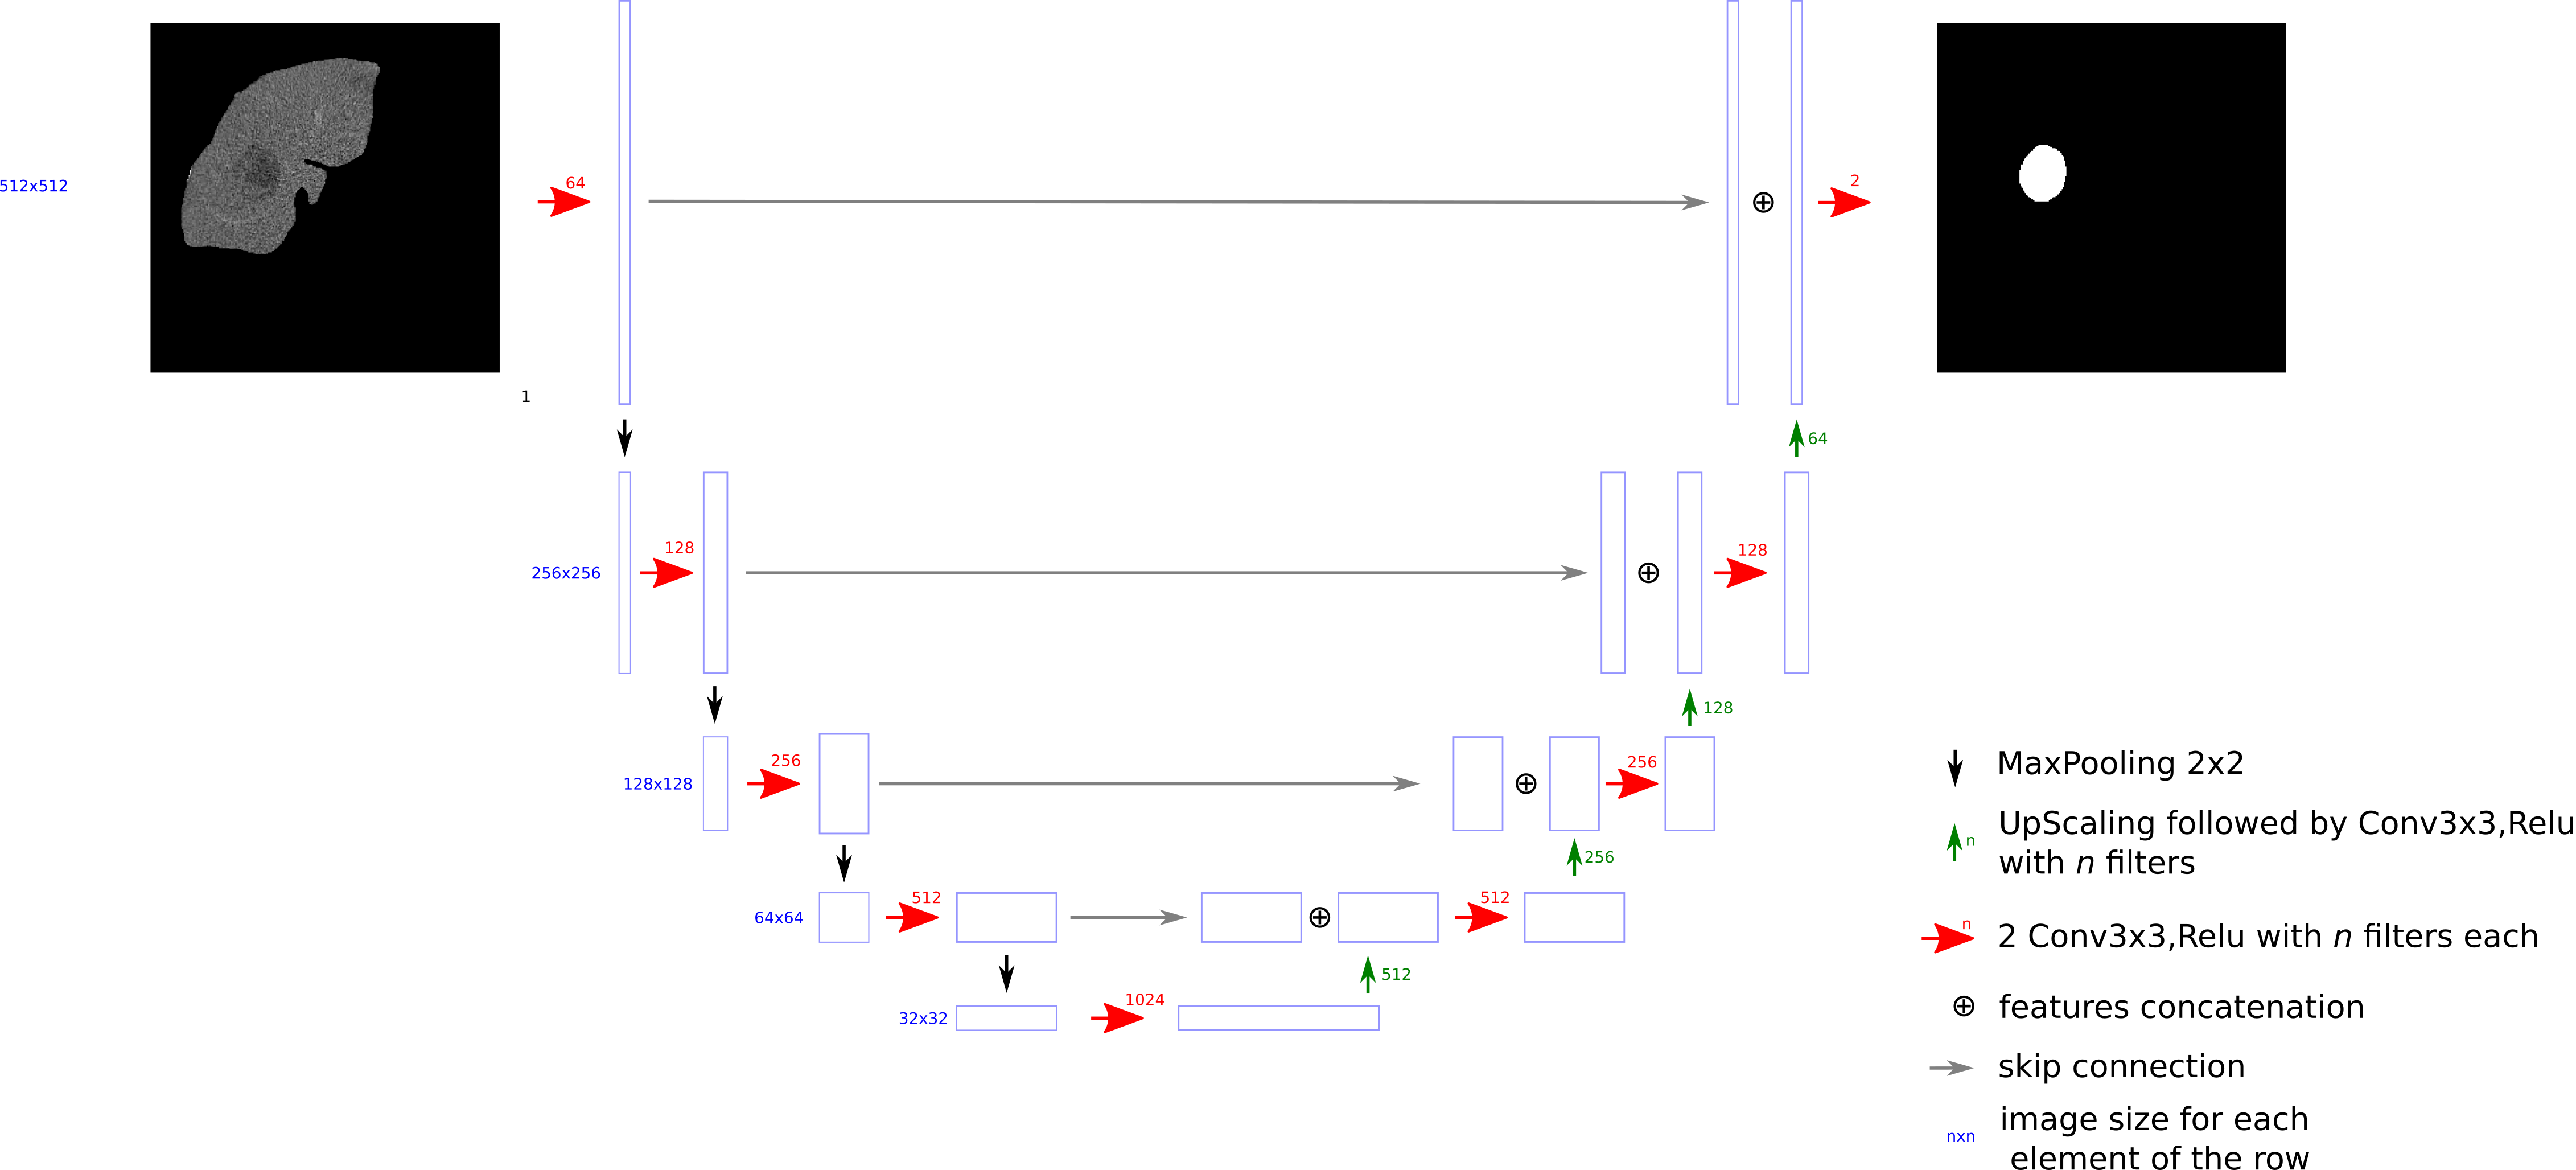
\includegraphics[width=0.9\linewidth]{../SemanticSeg/images/PV_Lesion}
	\caption{\pplfont{\ac{pv}-Lesion} network used to segment lesions within the liver with a \ac{pv} image as input}
	\label{CARS_PV_lesion_Fig}
\end{figure}


In order to evaluate the improvements brought by the cascaded
architecture, we also trained the original \emph{U-Net} architecture to
perform simultaneously the whole internal tissues segmentation task. The
same naming system as previously will be used where ``Full'' corresponds
to the simultaneous segmentation task, thus, \pplfont{AR-Full} will refer to the
network dedicated to the segmentation of both the parenchyma, the active
and the necrotic part of the lesions simultaneously, with AR
images as input. An illustration of the network is given in the figure
\ref{CARS_ArFull_Fig}.

\begin{figure}[th!]
	\centering
	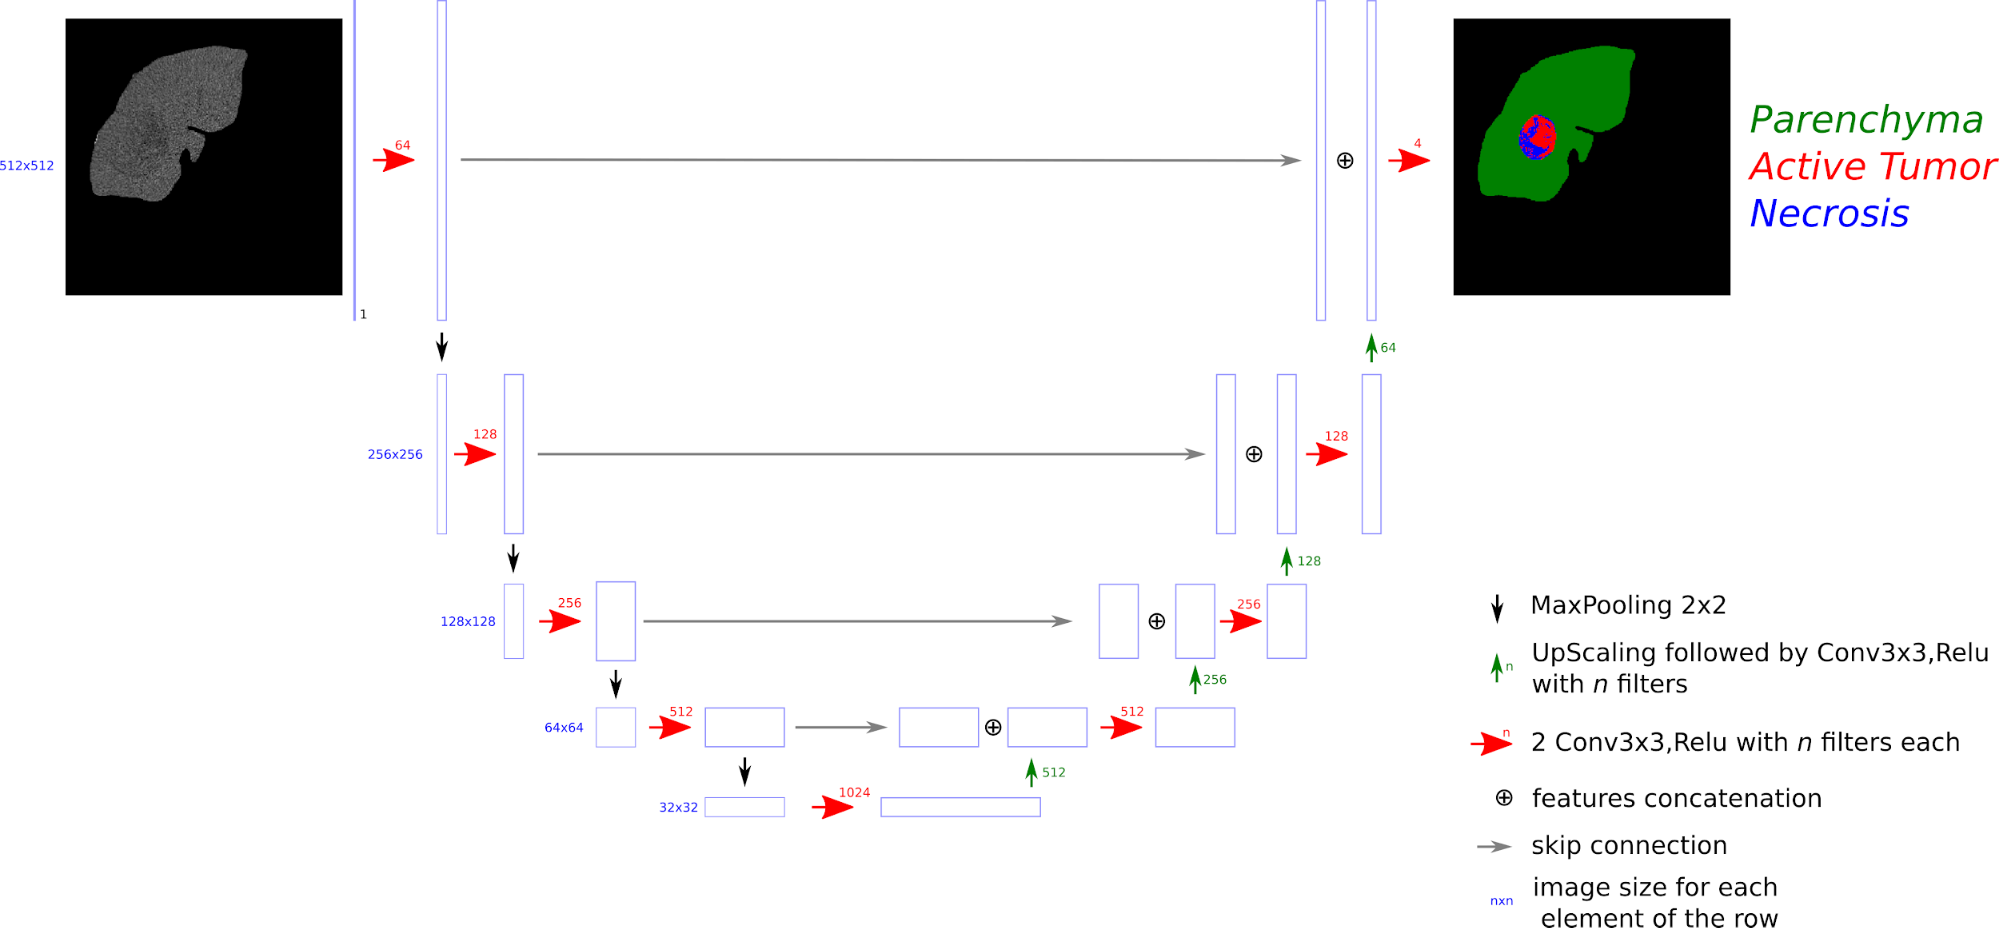
\includegraphics[width=0.9\linewidth]{../SemanticSeg/images/image23}
	\caption{\pplfont{AR-Full} refers to the network trained with AR images as input (values outside the liver are masked), and that outputs a label map, with parenchyma, active and necrotic parts annotated}
	\label{CARS_ArFull_Fig}
\end{figure}


\section{Multiphase information}

Only the \ac{ar} and \ac{pv} phases were considered in the
multiphase networks because \ac{nect} phase images do not provide enough
inter-tissue contrast. \\
In order to incorporate the multiphase information in our pipeline, we
investigated 2 different strategies. The first one, referred to as DMP (Dimensional MultiPhase), consists in concatenating both the
AR and \ac{pv} images as input to the network (see figure \ref{CARS_DMP_Full_Fig}).
The second one referred to as MPF (MultiPhase Fusion), consists
in performing both the encoding and the decoding separately for each
phase, before merging the output maps (simple addition on the obtained
features maps), as depicted in the figure \ref{CARS_MPF_Full_Fig}.

\begin{figure}[th!]
	\centering
	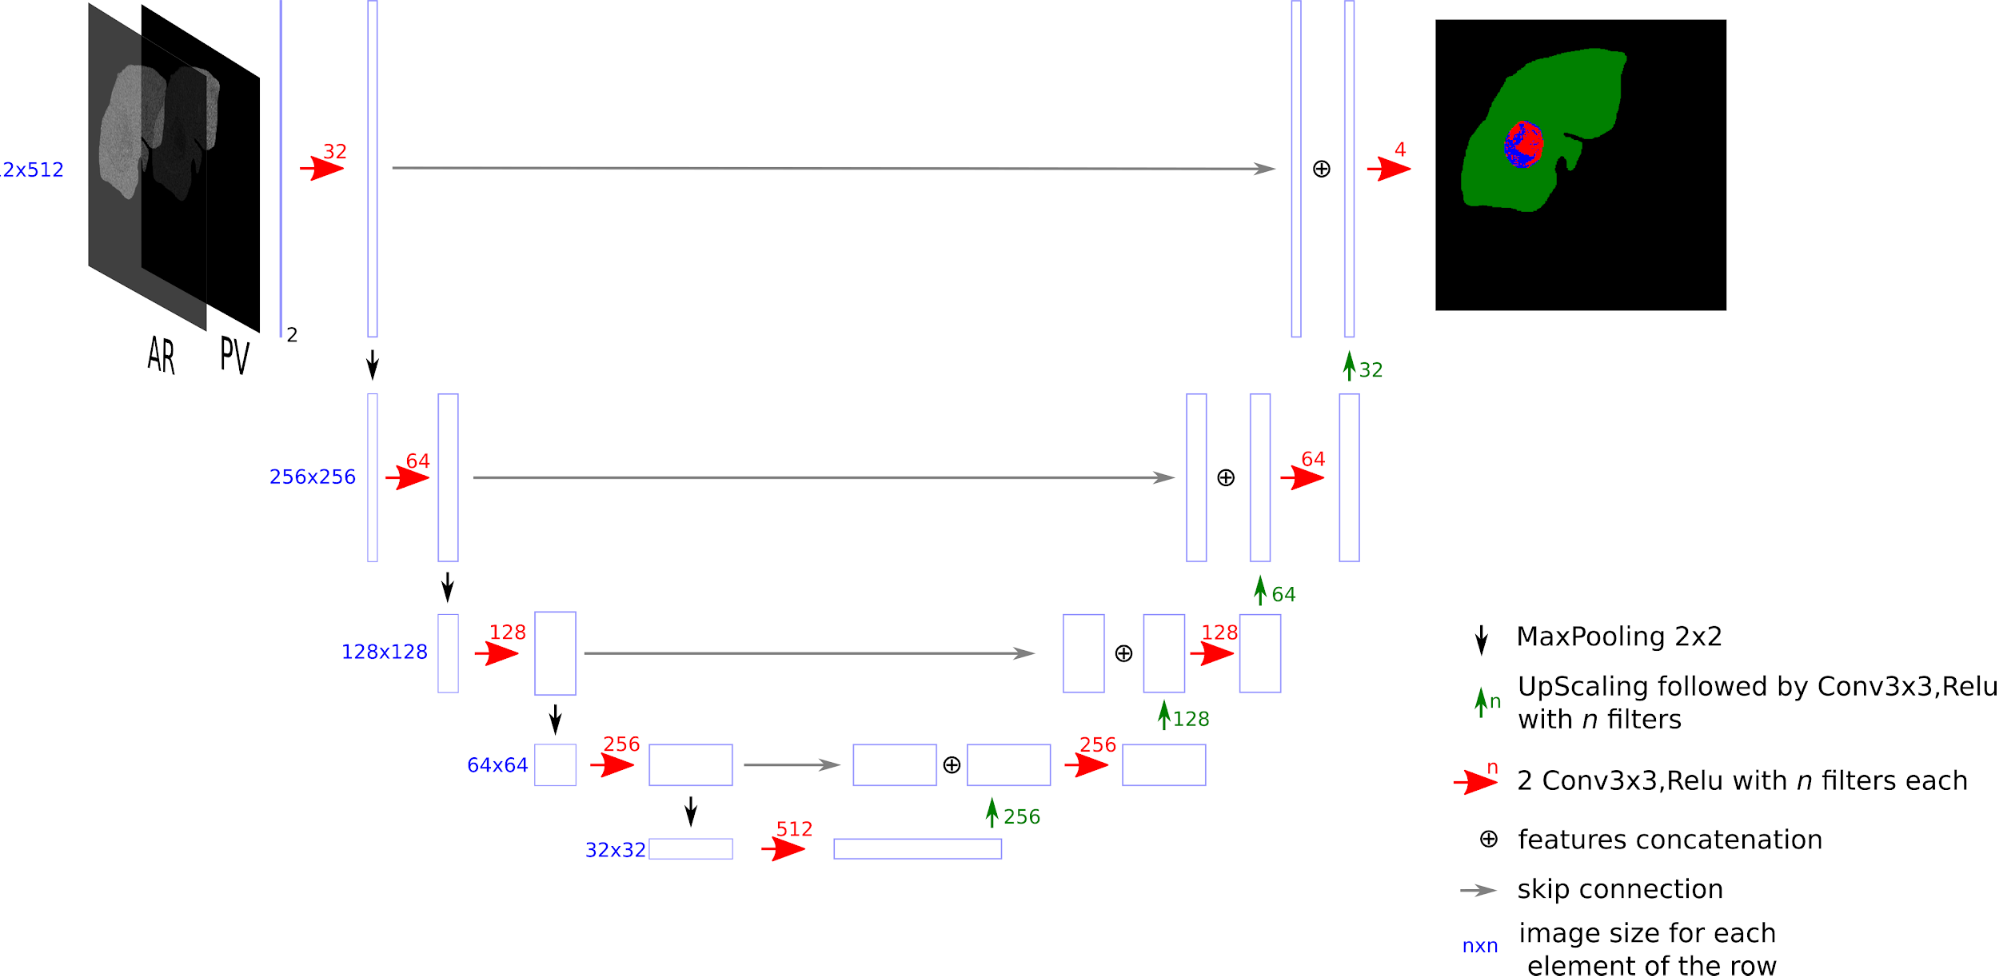
\includegraphics[width=0.9\linewidth]{../SemanticSeg/images/image28}
	\caption{\pplfont{DMP-Full} network that combines the AR and the \ac{pv} images as an input to segment the parenchyma and both the active and the necrotic parts of the lesions. Here, the two channels are considered as features for the first layer}
	\label{CARS_DMP_Full_Fig}
\end{figure}


\begin{figure}[th!]
	\centering
	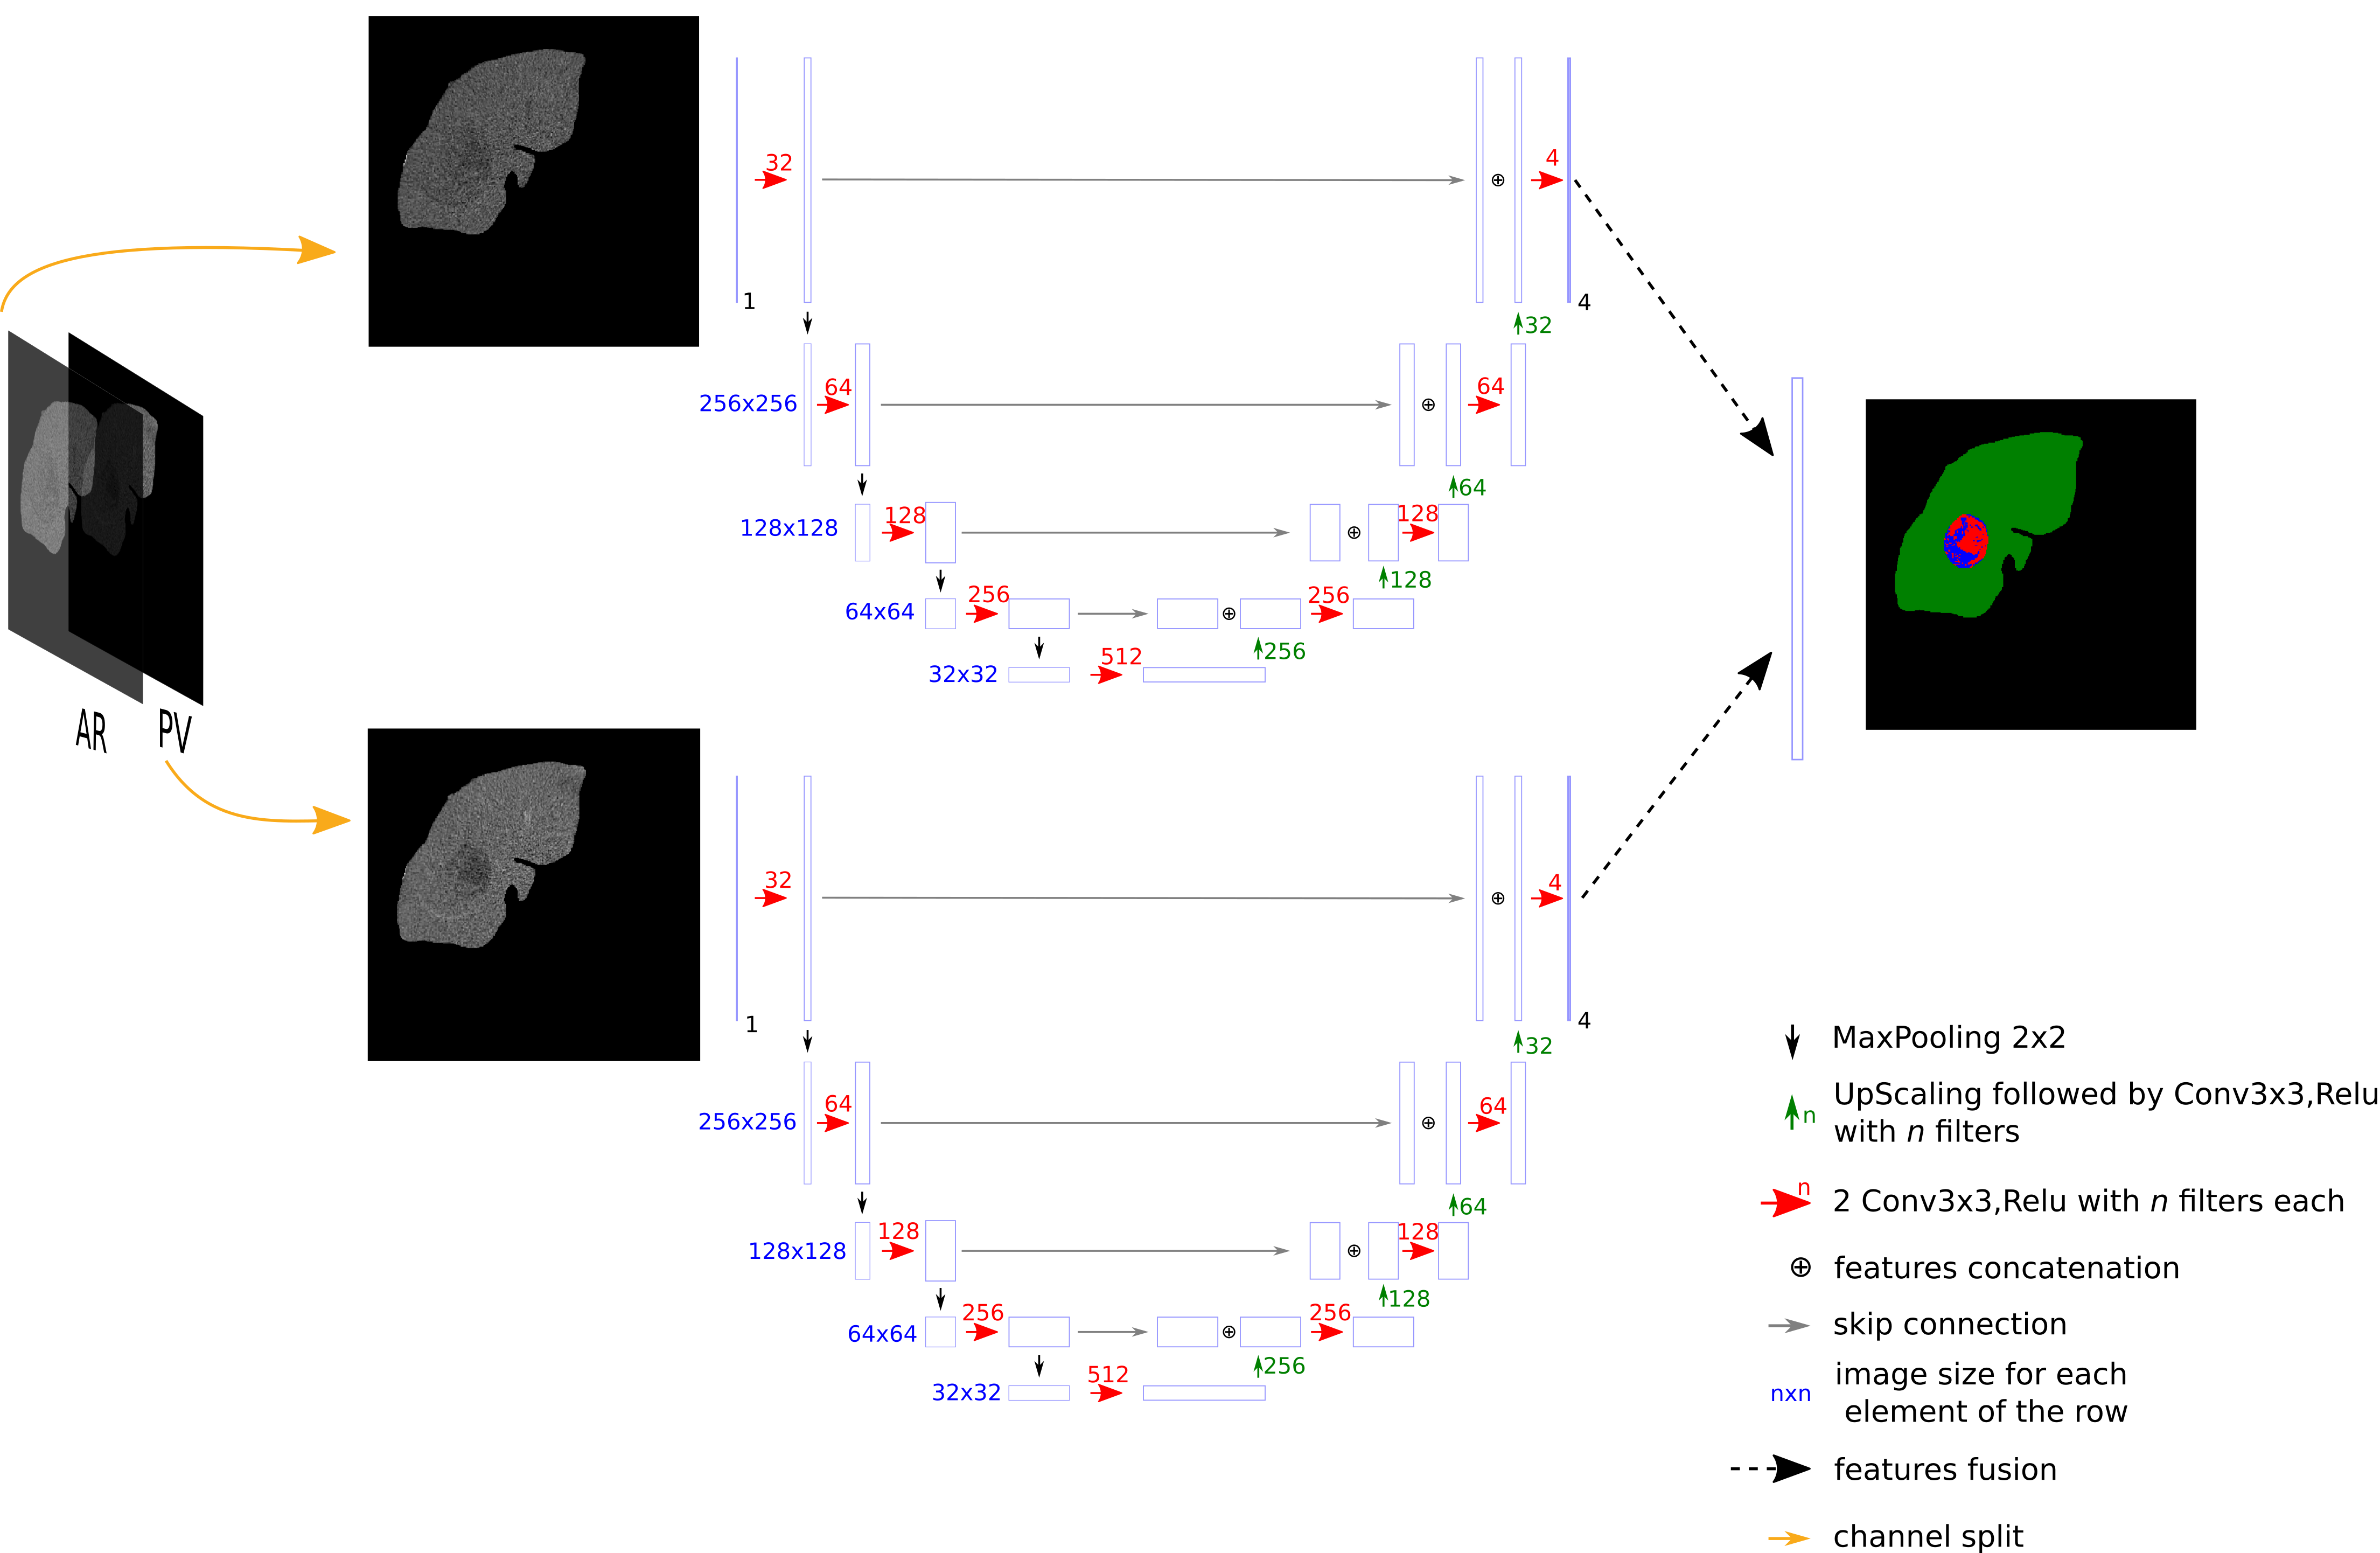
\includegraphics[width=0.9\linewidth]{../SemanticSeg/images/MPF_Full_8M_Resized_Font}
	\caption{\pplfont{MPF-Full} network: initially, AR and \ac{pv} images are processed separately. The resulting maps are merged (by simple addition) at the end}
	\label{CARS_MPF_Full_Fig}
\end{figure}



\section{Datasets}

The different datasets used in our research work are detailed in the
table \ref{xp_datasets}.

\renewcommand{\arraystretch}{2}
\setlength{\tabcolsep}{7pt}
\newgeometry{top=5mm, left=5mm, right=5mm, bottom=10mm, footskip=5mm, headsep=10mm}

\begin{landscape}
\scriptsize
	\begin{longtable}{l|p{2cm}p{1.5cm}p{1.6cm}p{3cm}p{1.5cm}p{1cm}p{1cm}p{1cm}p{1cm}p{1cm}p{1cm}}\toprule
		\textbf{Db Name} & \textbf{Db retained number of cases} & \textbf{Axial voxel size (mm)} & \textbf{Slice Thickness (mm)} & \textbf{Available contrast-enhanced phases} & \textbf{Contains Tumor} & \textbf{Tumor type} & \textbf{Liver  Ground truth} & \textbf{Tumor Ground truth} & \textbf{Necrosis Ground truth}& \textbf{\#Experts} \\
		\midrule
		\textbf{\lmttfont{TheraHCC-dB}} &104 2D slices &0.66-0.97 &0.7-1.25 &NECT, AR \& PV&Yes &HCC & true & true & true &4 \\
		\textbf{\lmttfont{LITS-dB}}& 131  3D vol. & 0.55-1 &0.45-6 &Single phase images but mixed (AR \& PV)&Yes &Mixed & true & true & false &3 \\
		\textbf{\lmttfont{3DIrcad-dB}}\footnote{Subset of the 3DIrcad-01 presented in the table \ref{publicly_available_datasets} where only the 15 volumes with liver tumors were retained} & 15 3D vol. &0.57-0.87 &1.25-4 &Single phase images but mixed (AR \& PV) &Yes &Mixed & true & true & false &- \\
		\textbf{\lmttfont{TCIA-dB}} \footnote{Subset of the one presented in the table \ref{publicly_available_datasets} where only the 18 exploitable volumes with both AR and PV phases were retained} & 18 3D vol. &0.62-0.90 &2.5-7 &AR\&PV&Yes&HCC & false & true & true &1 \\
		\textbf{\lmttfont{G-dB}} & 79  3D vol. &0.58-0.98 &0.8-5 &AR\&PV&Yes &HCC & false & true & false &1 \\
		\bottomrule
		\caption{Datasets used in our experiments (NECT: Non-Enhanced Contrast CT, AR: Arterial, PV: Portal Venous)}\label{xp_datasets}
	\end{longtable}
\end{landscape}

\renewcommand{\arraystretch}{5}
\newgeometry{vmargin={15mm}, hmargin={30mm,30mm}}   % set the margins 

As we can see in the table, and except for \textbf{\lmttfont{LITS-dB}} and \textbf{\lmttfont{3DIrcad-dB}}
(\textbf{\lmttfont{3DIrcad-dB}} being a subset of the \textbf{\lmttfont{LITS-dB}} \cite{Bilic2019}), they are all different in their construction. Differences can
be found on the annotated areas (chosen sparse slices or entire 3D
volumes) and on the annotated tissues that can be found in the dataset
(some of them only contain ground truth annotations for the liver and
the tumors it might contain such as \textbf{\lmttfont{LITS-dB}}, whereas some others contain
only ground truth annotation for the tumor such as \textbf{\lmttfont{TCIA-dB}}). Another
crucial difference concerns the contrast enhanced phases available in
each dataset (\textbf{\lmttfont{LITS-dB}} contains only single phase images whereas \textbf{\lmttfont{TCIA-dB}},
\textbf{\lmttfont{TheraHCC-dB}} and \textbf{\lmttfont{G-dB}} present multiphasic images). \\
To prove the ability of the deep learning to perform the automatic
segmentation of both the liver and its internal tissues, such as the
parenchyma and both the active and the necrotic part of the tumor, we
first performed our experiments on \textbf{\lmttfont{TheraHCC-dB}} since this database was
previously used for the same task \cite{Conze2017}, because it
presents multiphase images and finally because this is the only
available dataset with complete ground truth for both liver parenchyma,
active and necrotic part of the tumors. \\
%TheraHCC-dB has been chosen here for its high difference with the other 


\section{Experiments}

\subsection{Material}

\textbf{\lmttfont{TheraHCC-dB}} is composed of images from seven patients, all suffering
from \emph{HCC} and who underwent \ac{cect} (Contrast-Enhanced
Computed Tomography) examinations, resulting in a total of 13 \ac{ct}
sequences. \\
More details about the standard \ac{cect} examination protocol can be
found in the chapter \ref{ct-and-mr-imaging}. In our case, images were acquired at 4 different
moments: one before the injection of the contrast medium (\ac{nect}:
Non Enhanced \ac{ct}) , and the 2 others after the injection to reflect both
the arterial (\ac{ar}) (\textasciitilde{}20-25s after injection) and
the portal venous (\ac{pv}) phases (\textasciitilde{}60-70s after
injection).\\
Eight regularly sampled slices across each one the 13 sequences were
segmented by 4 experts, resulting in 104 labeled slices. \\
The segmentation maps obtained from each one the 4 experts were fused
using the STAPLE algorithm to reach a consensus map \cite{Warfield2004}.

\subsection{Data pre-processing}

The first task to implement in this study was the inter-phase
registration so that environmental effects, such as respiratory motions,
will not affect the performances of the networks, and to ensure that a
given voxel is at the exact same position for the different \ac{cect}
volumes of a patient. The registration was performed using a
diffeomorphic deformable registration algorithm, where the \ac{pv}
images were used as reference, since they contained the original expert
annotations \cite{Avants2008, Conze2017, Ben-Cohen, Christ2017}. \\
Another bias that can affect the deep semantic segmentation networks
training is the heterogeneous image sizes and voxel resolutions present
within the training images.
To avoid this bias, it has been decided to scale them so that they all
have a $ 512\times512 $ axial size \footnote{Either cropping or padding was performed so that the images have the same size} and an isotropic voxel resolution of $ 0.97 \text{mm}^2 $. \\
The data normalization is another aspect that needs to be considered
before feeding the images in the deep network. In order to reduce the
effect of extreme values from regions present in the tomographic images
(such as the bones or the air), and to enhance the intensity of the
liver voxels, we first clipped the \emph{HU} values to be in the range
$ \left[-100, 400\right] $ , corresponding to the most commonly 
observed liver intensities range. The retained intensities were finally mapped to
the interval $ \left[0, 1\right]$ \footnote{\ac{dl} studies usually tend to perform 
data standardization but here HU values are already normalized. 
The used range helps us to avoid potential bias caused by images acquired at a delayed phase with a different contrast}.

\subsection{Training}\label{sem-seg-training}

In order to validate our hypotheses, we have decided to first run
experiments on the \lmttfont{3DIrcad-dB} to set the most crucial hyperparameters
such as the learning rate, the decay, the depth of the network or the
type and the amount of data augmentation.
The selection process is detailed in the appendix \ref{appendix---hyperparameters-selection}, and here is the list of the chosen hyperparameters:

\begin{itemize}
	\item Lr: 1e-4
	\item Decay: 1e-4
	\item Number of epochs: 20
	\item Optimizer: Adam
	\item Number of filters at bottleneck: 1024
	\item Input image size: 512
	\item Data augmentation
	\begin{itemize}
		\item Rotations in the interval $ \left[0, 40\right] $
		\item Translations with shift in the interval $ \left[-0.1, 0.1\right] $
		\item Horizontal and vertical flips
	\end{itemize}
	\item Augmentation factor: 20
\end{itemize}

When transferring those settings to the \textbf{\lmttfont{TheraHCC-dB}}, 
we implemented both translation and the addition of gaussian
noise in the training since it slightly improved the performances.
In order to remove any bias, the same set of hyperparameters has been
used for both the \pplfont{\{.\}-Liver}, \pplfont{\{.\}-Lesion}, \pplfont{\{.\}-Necrosis} and
\pplfont{\{.\}-Full} networks when training the \textbf{\lmttfont{TheraHCC-dB}}, regardless of the
type of input (single phase or multiphase). \\
%%%%%%%%%%%%%%%%%%%%
%Revised --> ADDED
%%%%%%%%%%%%%%%%%%%%
\textcolor{red}{The original U-Net architecture implemented by Ronneberger et al. had a total of 32M parameters, and the results obtained when setting the hyperparameters tend also to prove that the best results were obtained using an architecture with the same number of parameters (with 1024 filters at bottleneck as mentioned above). When performing the segmentation of both the necrotic and the active parts of the tumor from a masked liver image, our cascaded version consists of 2 concatenated U-Net networks (one to segment the tumor and the second to differentiate between the active and the necrotic part) therefore, we decided to reduce the number of parameters to 8M parameters for each network of the cascaded (512 filters used at bottleneck instead of 1024) in comparison with the versatile networks (which have a total of 32M parameters) to ensure that no bias existed in favor of the cascaded networks.
Only the \pplfont{MPF-\{.\}} had a total of 16M parameters since it already consists of 2 combined U-Net networks as illustrated in the figure \ref{CARS_MPF_Full_Fig}.
To cope with the high imbalanced data present in our datasets (e.g. number of voxels belonging to the tumor class vs those belonging to the parenchyma class when segmenting the lesion in the liver), we considered the weighted cross-entropy function as loss function when training our network. 
\begin{equation}
L = -\frac{1}{n} \sum_{i=1}^{N}\omega_i^{class}\left[\hat{P_i} \log P_i + (-\hat{P_i})\log (1 - P_i)\right]
\end{equation}
}

%%%%%%%%%%%%%%%%%%%%
%Revised --> REMOVED
%%%%%%%%%%%%%%%%%%%%
%The same set of hyperparameters was used to train both liver and lesions segmentation networks on respectively the \textbf{\lmttfont{LITS-dB}} and the \textbf{\lmttfont{G-dB}}.

%We first present the results obtain when performing the semantic segmentation of liver tissues on the \textbf{\lmttfont{TheraHCC-dB}}, before applied the resulting architecture to provide additional annotations to both \textbf{\lmttfont{TCIA-dB}} and \textbf{\lmttfont{G-dB}}.


\subsection{Semantic segmentation of liver tissues}

In this section, mean \ac{dsc}s were computed in a slice-wise fashion for each target class and the different methods were statistically compared using the Wilcoxon 
signed paired rank tests, since slice-wise \ac{dsc}s did not follow a normal distribution. 
We first compared \pplfont{\{\ac{nect}, \ac{ar}, \ac{pv}, DMP, MPF\}-Liver} networks
 to evaluate which phase allows better liver segmentation. 
 We then trained \pplfont{\{\ac{nect}, \ac{ar}, \ac{pv}, DMP, MPF\}-Lesion} and  \pplfont{\{\ac{nect}, \ac{ar}, \ac{pv}, DMP, MPF\}-Necrosis} networks separately on the \textbf{\lmttfont{TheraHCC-dB}} by masking all values outside the liver using ground truth annotations in order to assess whether multiphase information is really useful for the segmentation. The results are given in table \ref{SingleVsMult}.

Multiphase performed significantly better than single-phase for segmenting the liver (DMP vs \ac{pv}, $P=0.001$; DMP vs \ac{ar}, $P=0.005$, DMP vs \ac{nect}, $P<0.001$) and the active part of the lesions (DMP vs \ac{pv}, $P<0.001$; DMP vs \ac{ar}, $P=0.003$; DMP vs \ac{nect}, $P<0.001$). When comparing single-phase alone, \ac{pv} achieved significantly better \ac{dsc}s than \ac{ar} or \ac{nect} for all the segmentation tasks except for the liver segmentation. When comparing multiphase methods, DMP carries out significantly better than MPF for the segmentation of the liver (DMP vs MPF, $P=0.004$), the parenchyma (DMP vs MPF, $P<0.001$) and the active part of the lesions (DMP vs MPF, $P=0.005$).

Since both \pplfont{DMP-Lesion} and \pplfont{DMP-Necrosis} led to the best results, we combined them in a cascade as explained before, and compared it to both \pplfont{\{\ac{nect}, \ac{ar}, \ac{pv}, DMP, MPF\}-Full} networks. We evaluated them in terms of liver tissue classification performance on images where the values outside the ground truth liver area were masked. The mean \ac{dsc}s are reported in table \ref{FullvsCascade}. Examples of segmentation results are given in figure \ref{CompareFullCascade}. \\

\renewcommand{\arraystretch}{1}
\begin{table}[ht!]
\caption{Segmentation results using single-phase vs multiphase methods on \lmttfont{TheraHCC-dB}.}
\begin{tabular}{llccccc}
\cline{1-7}
\multicolumn{1}{l}{Input}& \multicolumn{1}{l}{Target} & \multicolumn{5}{l}{Network} \\
\cline{3-7}
\multicolumn{1}{c}{}& \multicolumn{1}{c}{} & \multicolumn{1}{c}{\pplfont{\ac{nect}}} & \multicolumn{1}{c}{\pplfont{\ac{ar}}} & \multicolumn{1}{c}{\pplfont{\ac{pv}}} & \multicolumn{1}{c}{\pplfont{DMP}} & \multicolumn{1}{c}{\pplfont{MPF}} \\
\cline{1-7}
Raw \ac{ct} & Liver & 81.1 $\pm$ 27.7 & 89.5 $\pm$ 13.2 & 88.7 $\pm$ 11.4 & $\mathbf{89.9 \pm 15.6}$ & 88.2 $\pm$ 16.0 \\
True liver mask & Parenchyma & 86.5 $\pm$ 13.7 & 82.5 $\pm$ 18.6 & 88.7 $\pm$ 15.4 & $\mathbf{90.5 \pm 13.2}$ & 86.9 $\pm$ 17.8 \\
True liver mask & Lesion & 77.4 $\pm$ 24.1 & 77.4 $\pm$ 20.2 & 87.8 $\pm$ 9.7 & $\mathbf{88.5 \pm 11.7}$ & 86.6 $\pm$ 10.3 \\

True lesion mask & Necrosis & 67.5 $\pm$ 15.5 & 69.7 $\pm$ 16.3  & 77.8 $\pm$ 12.4 & 78.5 $\pm$ 13.3 & $\mathbf{78.8 \pm 11.7}$ \\
True lesion mask & Active Tumor & 65.6 $\pm$ 20.4 & 63.9 $\pm$ 22.6 & 71.6 $\pm$ 20.7 & $\mathbf{75.5 \pm 17.4}$ & 73.2 $\pm$ 18.6 \\
\cline{1-7}
\end{tabular}
\label{SingleVsMult}
\end{table}

\begin{table}[ht!]
\caption{Segmentation results using \pplfont{\{$ \cdot$\}-Full} vs cascaded architectures on \lmttfont{TheraHCC-dB}.}
\begin{tabular}{lcccccc}
\cline{1-7}
\multicolumn{1}{l}{Target} & \multicolumn{6}{l}{Network} \\
\cline{2-7}
\multicolumn{1}{c}{}& \multicolumn{1}{c}{\pplfont{\ac{nect}-Full}} & \multicolumn{1}{c}{\pplfont{\ac{ar}-Full}} & \multicolumn{1}{c}{\pplfont{\ac{pv}-Full}} & \multicolumn{1}{c}{\pplfont{DMP-Full}} & \multicolumn{1}{c}{\pplfont{MPF-Full}} &
\multicolumn{1}{c}{Cascaded DMP}\\
\cline{1-7}
Parenchyma & 85.3 $\pm$ 14.9 & 84.1 $\pm$ 17.9 & 87.0 $\pm$ 19.0  & 82.9 $\pm$ 19.7 & 87.9 $\pm$ 15.9 & $\mathbf{90.5 \pm 13.2}$\\
Necrosis & 62.6 $\pm$ 18.6 & 63.5 $\pm$ 21.5 & 75.7 $\pm$ 14.4 & 73.7 $\pm$ 14.1 & 75.6 $\pm$ 13.4 & $\mathbf{75.8 \pm 15.1}$ \\
Active Tumor & 42.2 $\pm$ 24.0 & 43.2 $\pm$ 26.1 & 53.5 $\pm$ 24.2 & 51.3 $\pm$ 25.6 & 52.0 $\pm$ 23.3 & $\mathbf{59.6 \pm 22.5}$ \\
\cline{1-7}
\end{tabular}
\label{FullvsCascade}
\end{table}

The results highlighted that the cascaded version performed significantly better than \pplfont{\{$ \cdot$\}-Full} networks for segmenting the active part of the lesion (Cascaded DMP vs \pplfont{\ac{pv}-Full}, $P = 0.001$).
The resulting segmentation maps allow us to estimate the necrosis rate (which will be the ratio between the necrotic and the tumor areas). This metric is commonly used for diagnosis and prognosis of the treatment outcome. In this configuration\footnote{after using the liver expert \ac{gt} as mask for the first step}, our workflow provided estimates of this valuable biomarker with a mean error rate of 13.0 \%, which is accurate enough for clinical application. \\

When compared with another study that have been using a different dataset composed of MR images, we achieved slightly better segmentation results \cite{Zhang}.
We evaluated our method on the same database used in \cite{Conze2017}, where a manual expert interaction was required for the segmentation phase, which is not the case in the present deep learning approach. To allow fair comparison, the evaluation was conducted on the areas where all the experts reached an agreement as in \cite{Conze2017}. The mean patient-wise segmentation \ac{dsc}s are depicted in table \ref{ComparisionConze}. Our method enabled a better segmentation of the lesions and both necrotic and active parts. Therefore, we were able to predict the patient-wise necrosis rate with a slightly better precision. 

\begin{table}[ht!]
\caption{Average patient-wise segmentation \ac{dsc}s (on full agreement expert area) with the semi-interactive approach of \cite{Conze2017} and the cascaded DMP method}
\begin{tabular}{lcc}
\hline
& Semi-interactive method \cite{Conze2017} & ours \\
\hline
Parenchyma & \textbf{93.7 $\pm$ 3.4} & 92.2 $\pm$ 4.7 \\
Lesion & 90.7 $\pm$ 6 & \textbf{91.8 $\pm$ 4} \\
Necrosis & 83.0 $\pm$ 12.9 & \textbf{83.6 $\pm$ 11.7} \\
Active Tumor & 75.2 $\pm$ 10.9 & \textbf{82.0 $\pm$ 6.4} \\
Necrosis rate error & 7.84 $\pm$ 4.4 & \textbf{7.10 $\pm$ 1.4} \\
\hline
\end{tabular}
\label{ComparisionConze}
\end{table}

\begin{figure}[!ht]
\centering
\begin{minipage}{4cm}
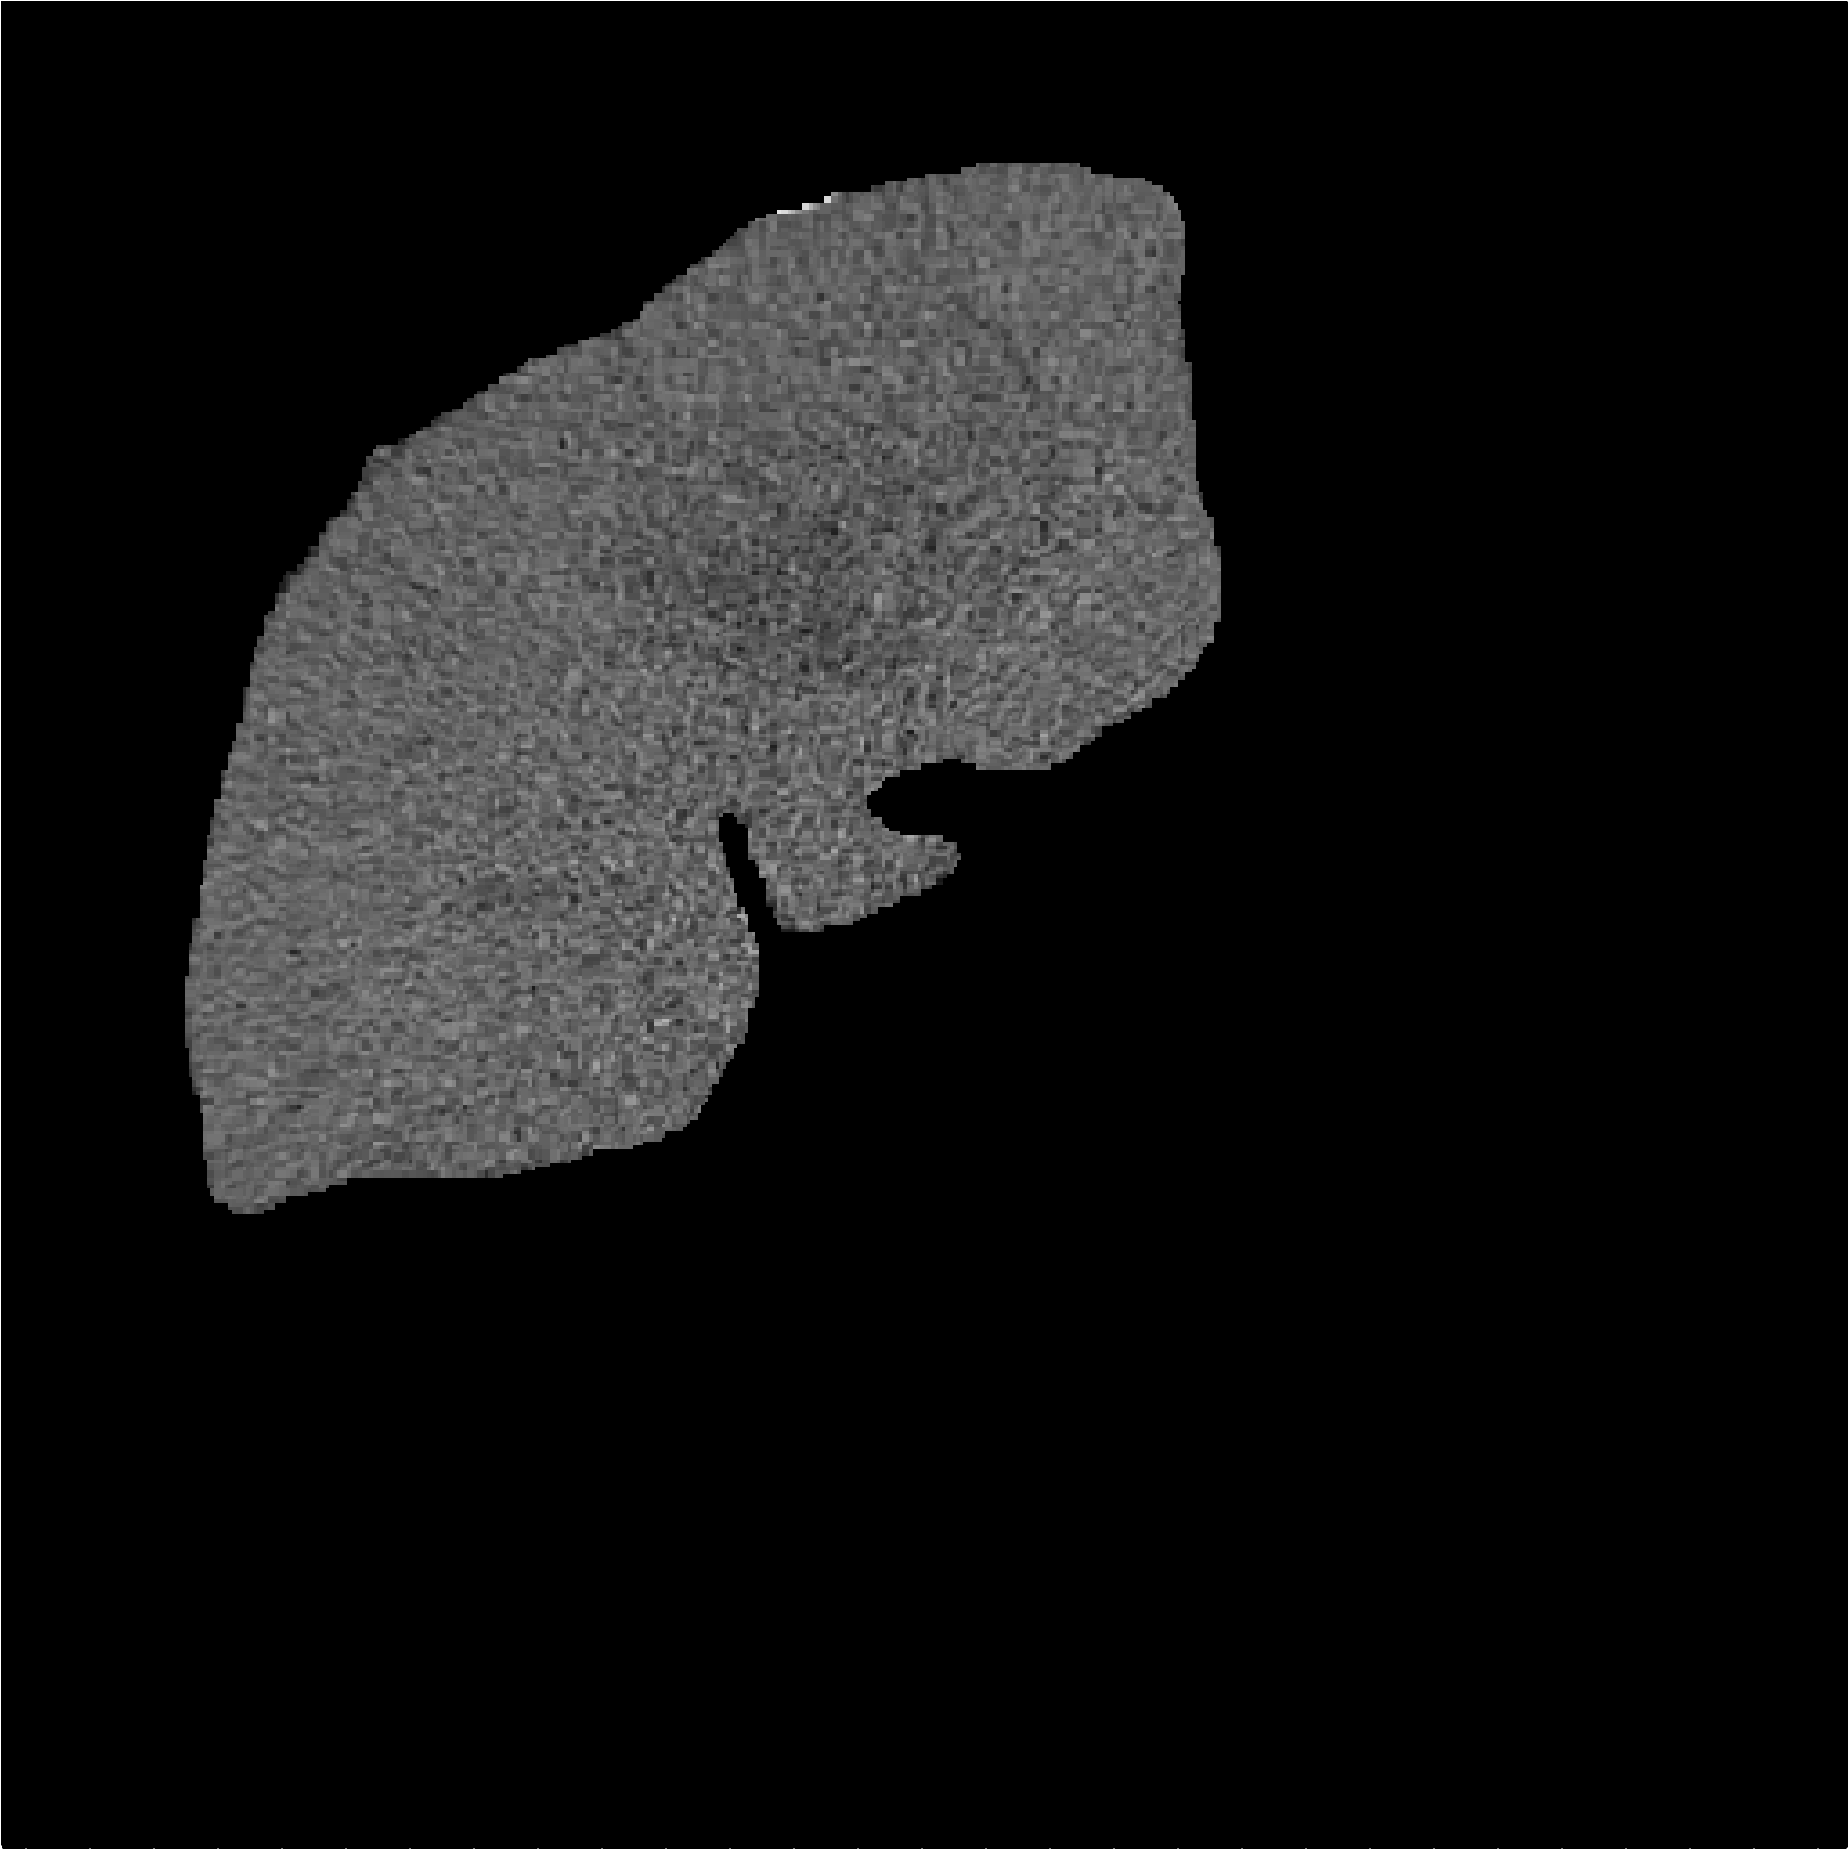
\includegraphics[width=\linewidth]{../SemanticSeg/images/1_21_orig_resized}
\end{minipage} \hspace{-0.3cm}
\begin{minipage}{4cm}
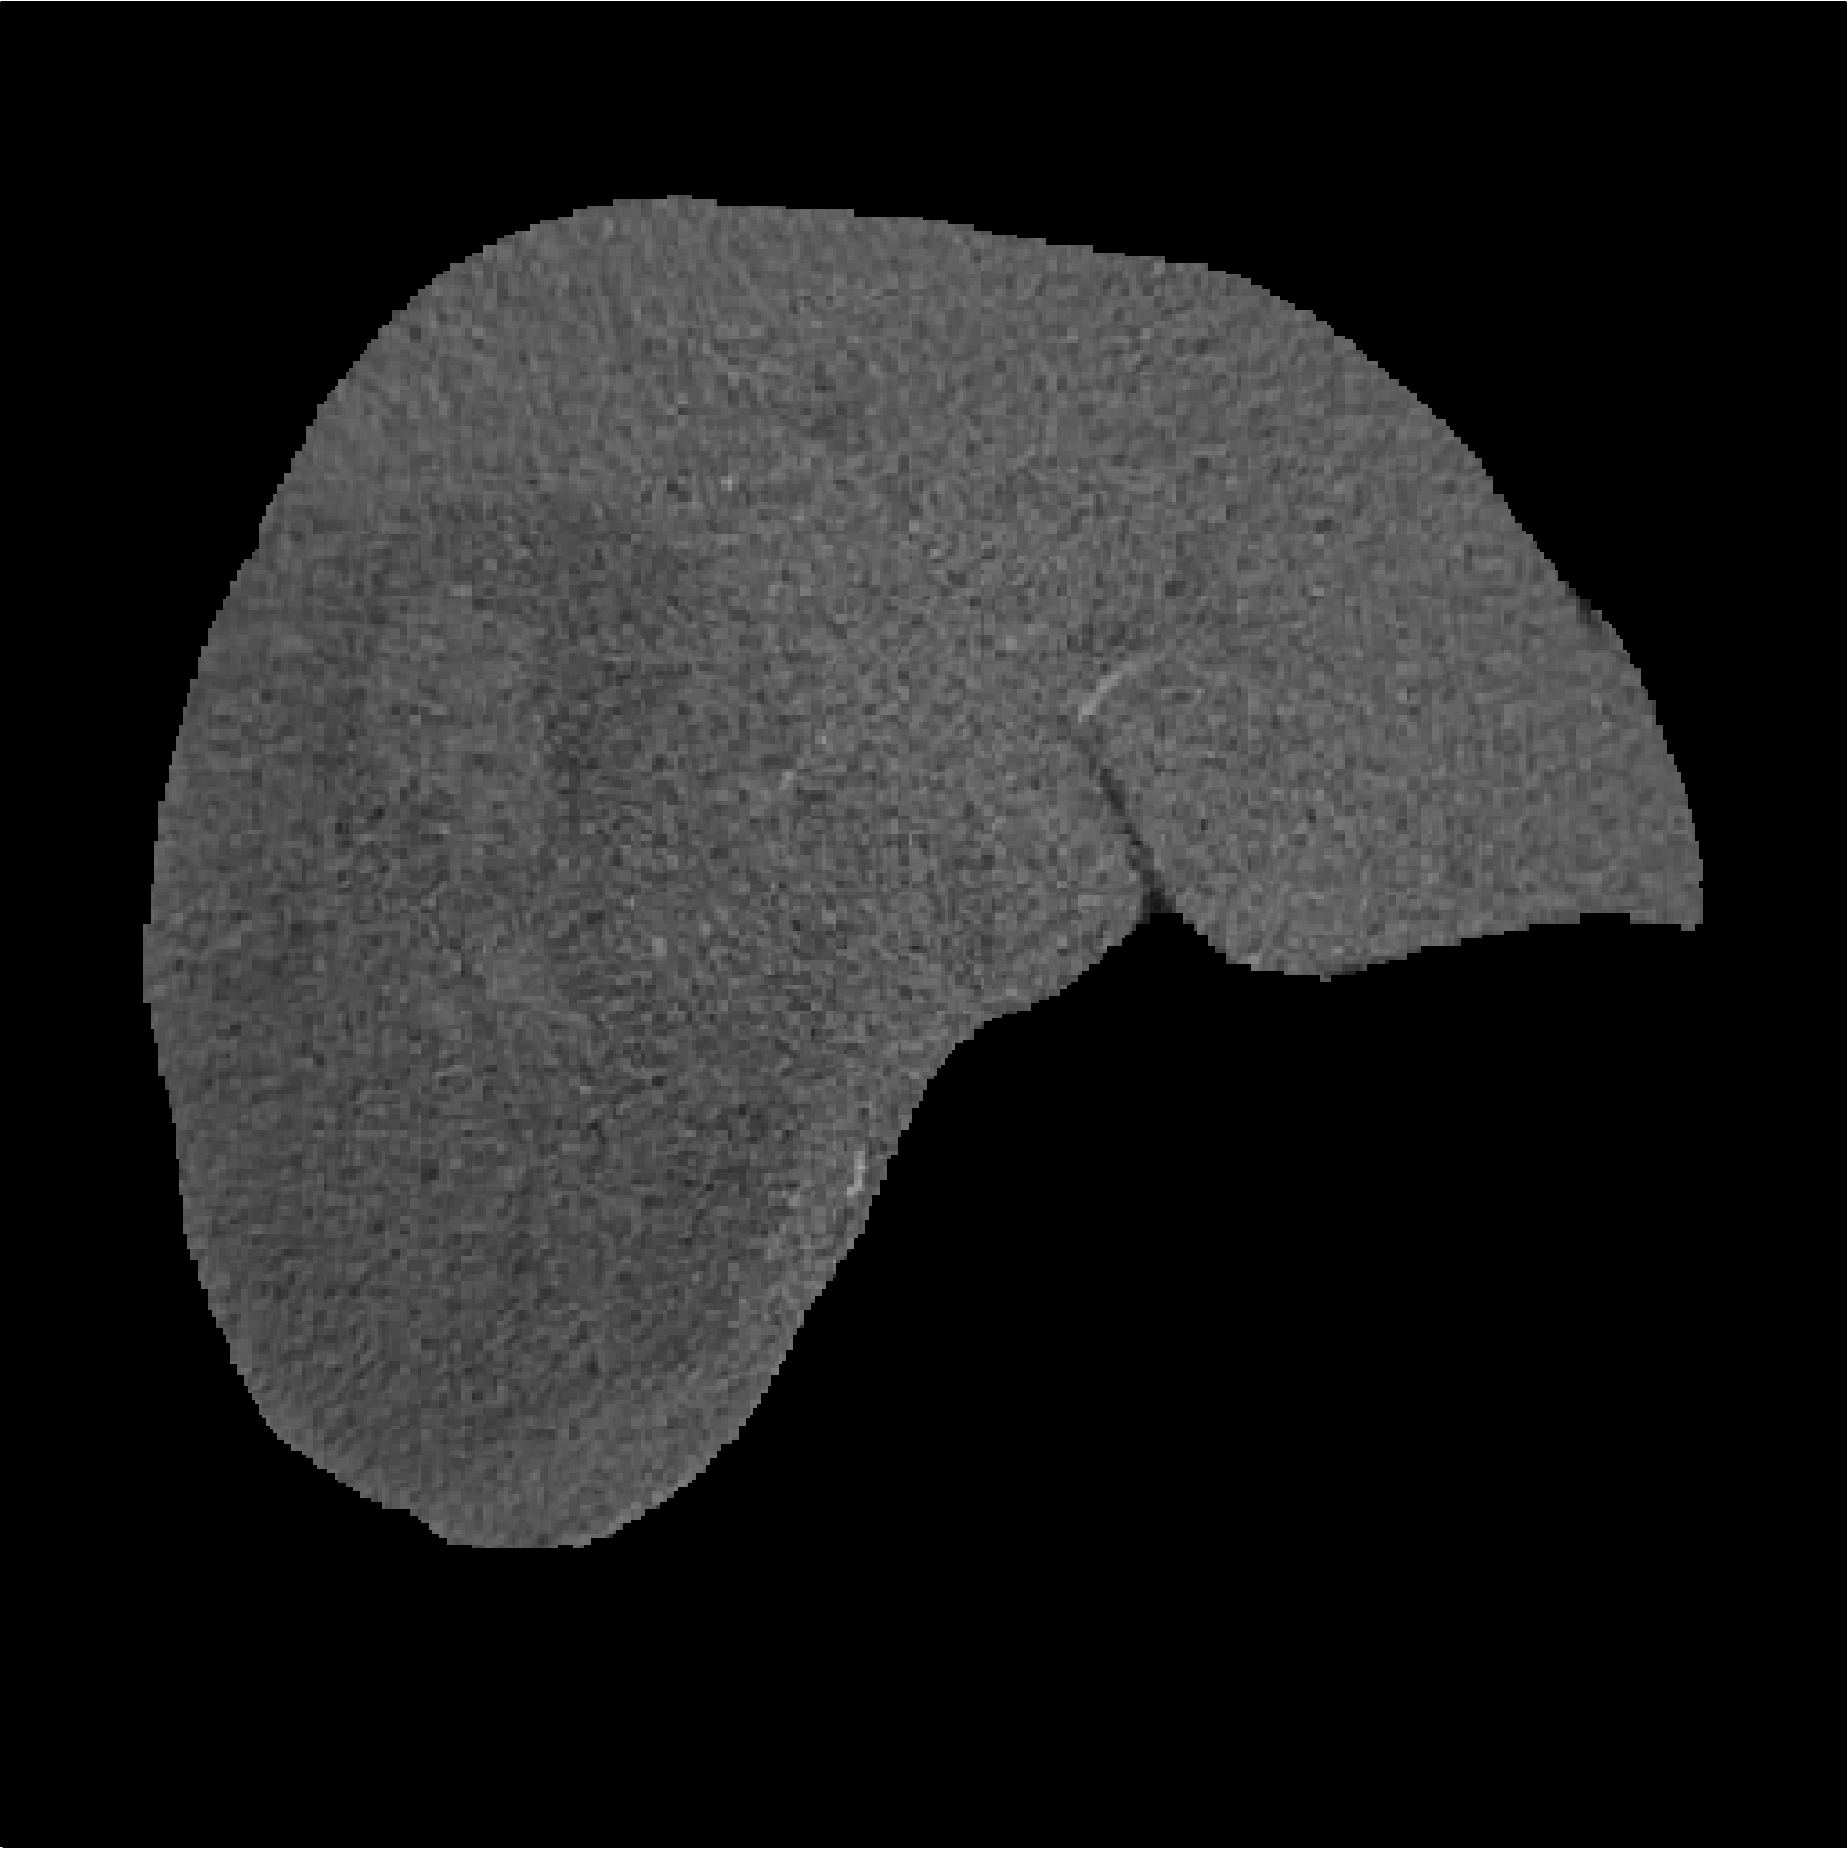
\includegraphics[width=\linewidth]{../SemanticSeg/images/5_2_orig_resized}
\end{minipage} \hspace{-0.3cm}
\begin{minipage}{4cm}
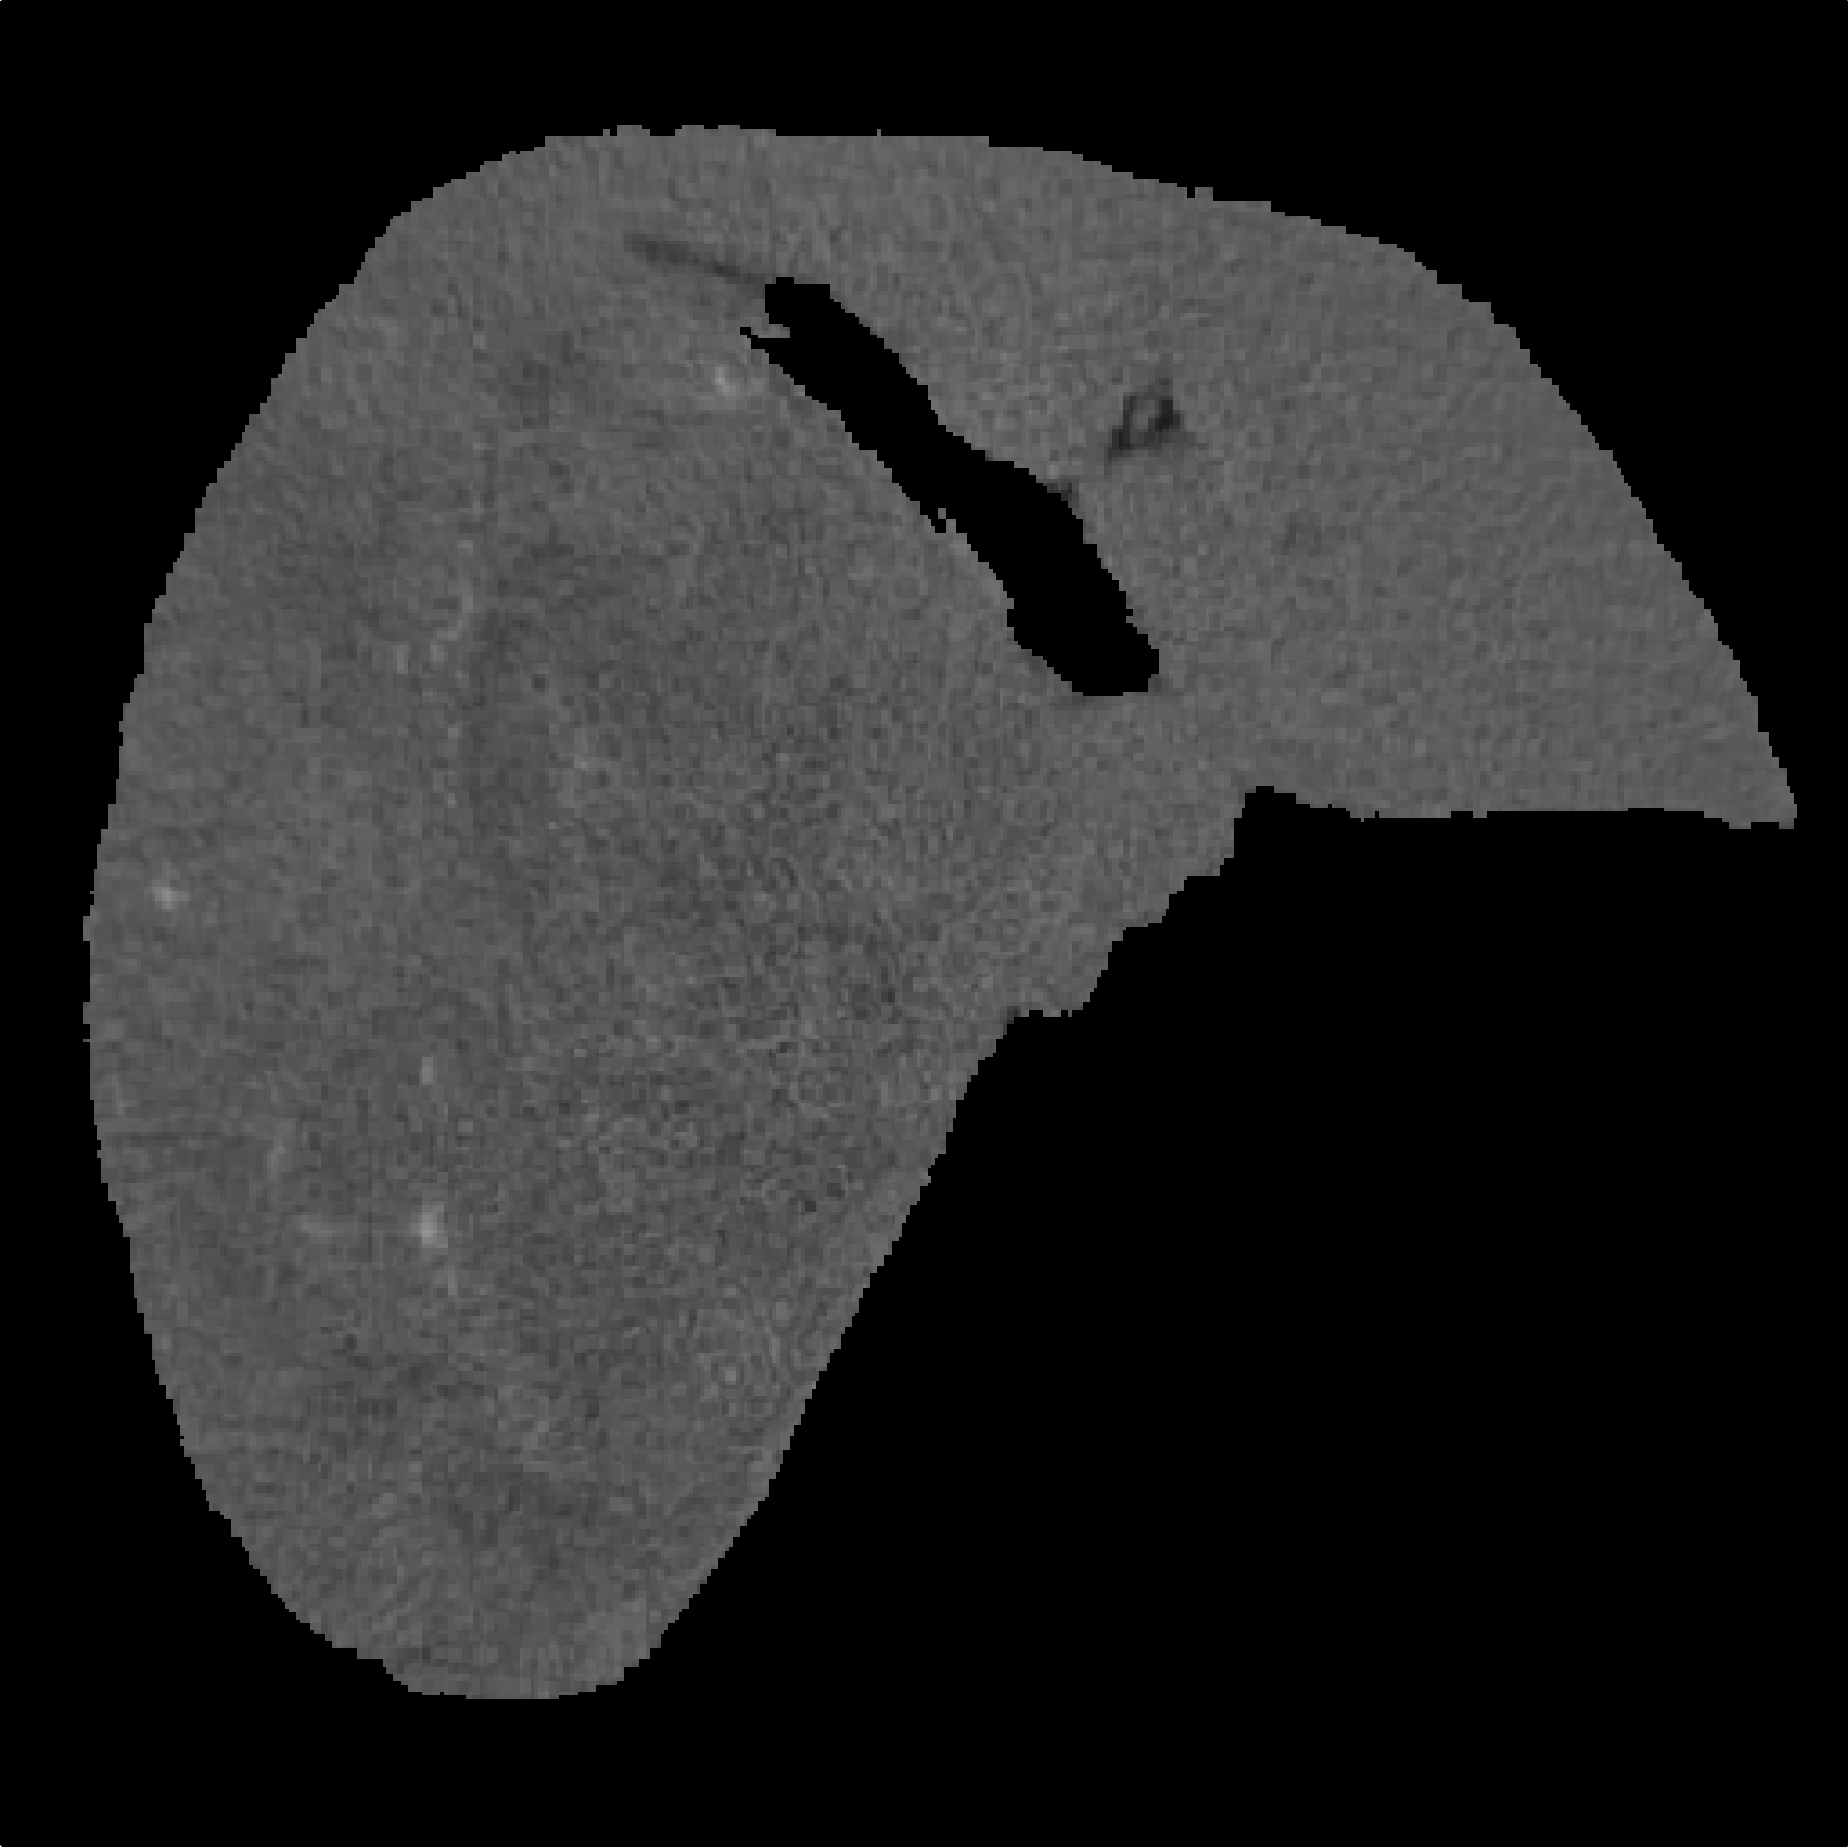
\includegraphics[width=\linewidth]{../SemanticSeg/images/5_8_orig_resized}
\end{minipage}
\vspace{-0.2cm}
\begin{minipage}{4cm}
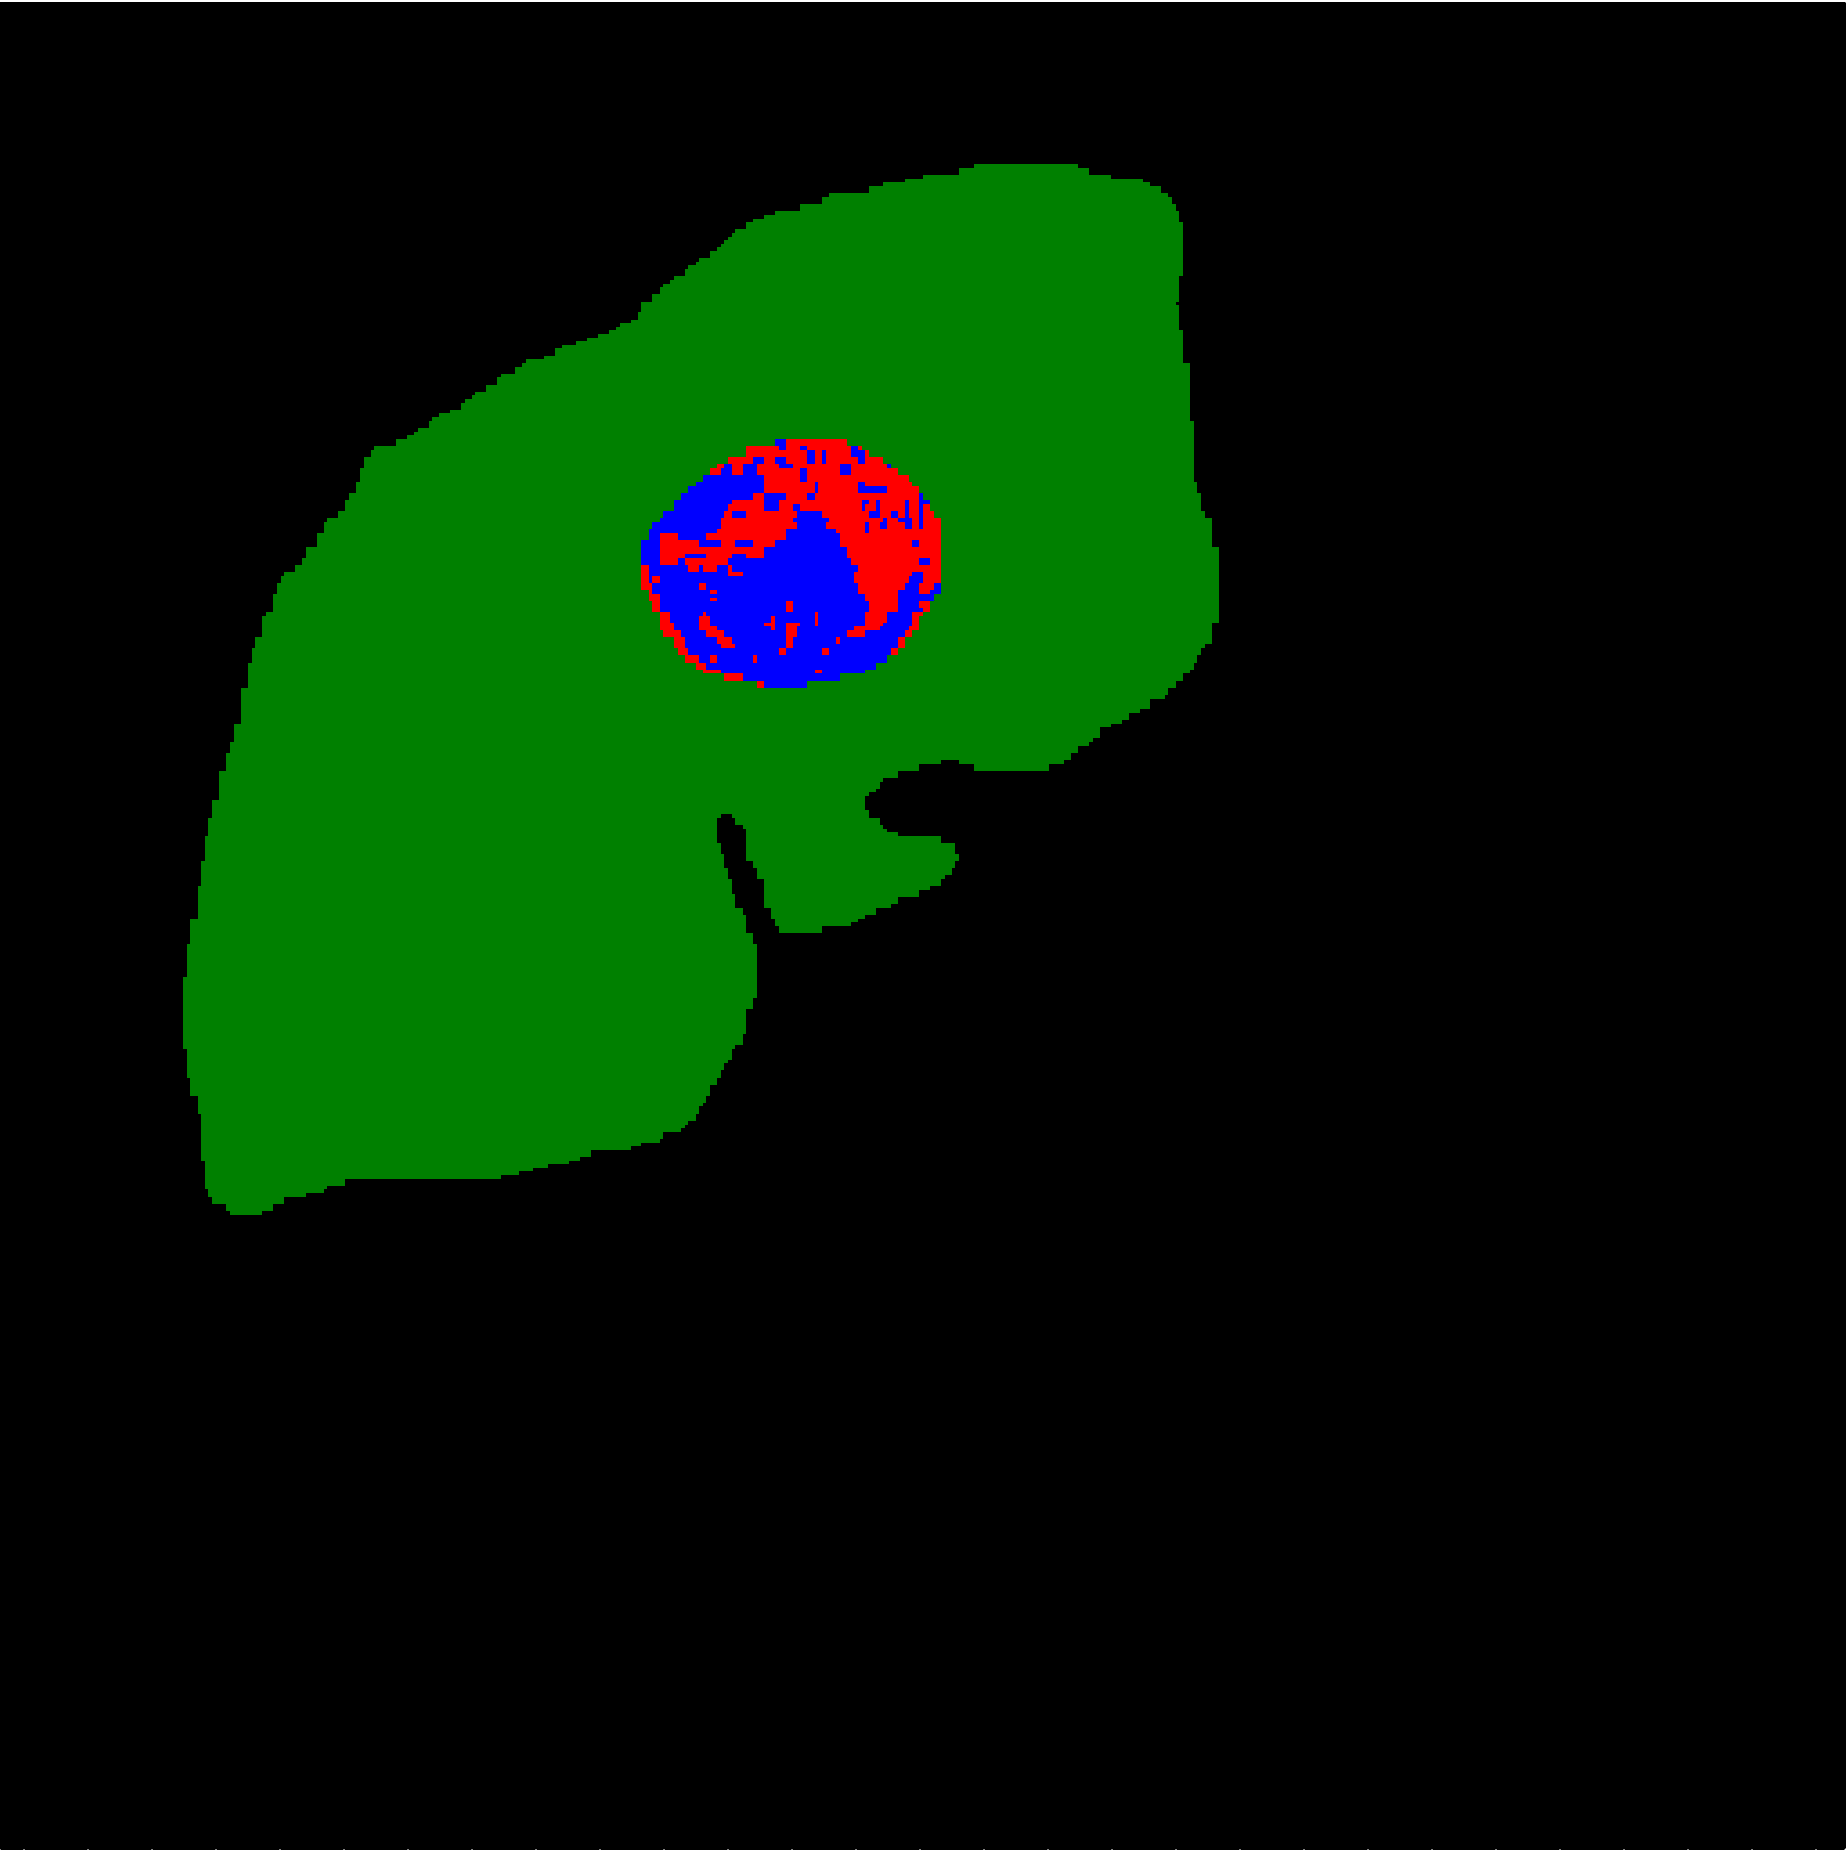
\includegraphics[width=\linewidth]{../SemanticSeg/images/1_21_gt_resized}
\end{minipage} \hspace{-0.3cm}
\begin{minipage}{4cm}
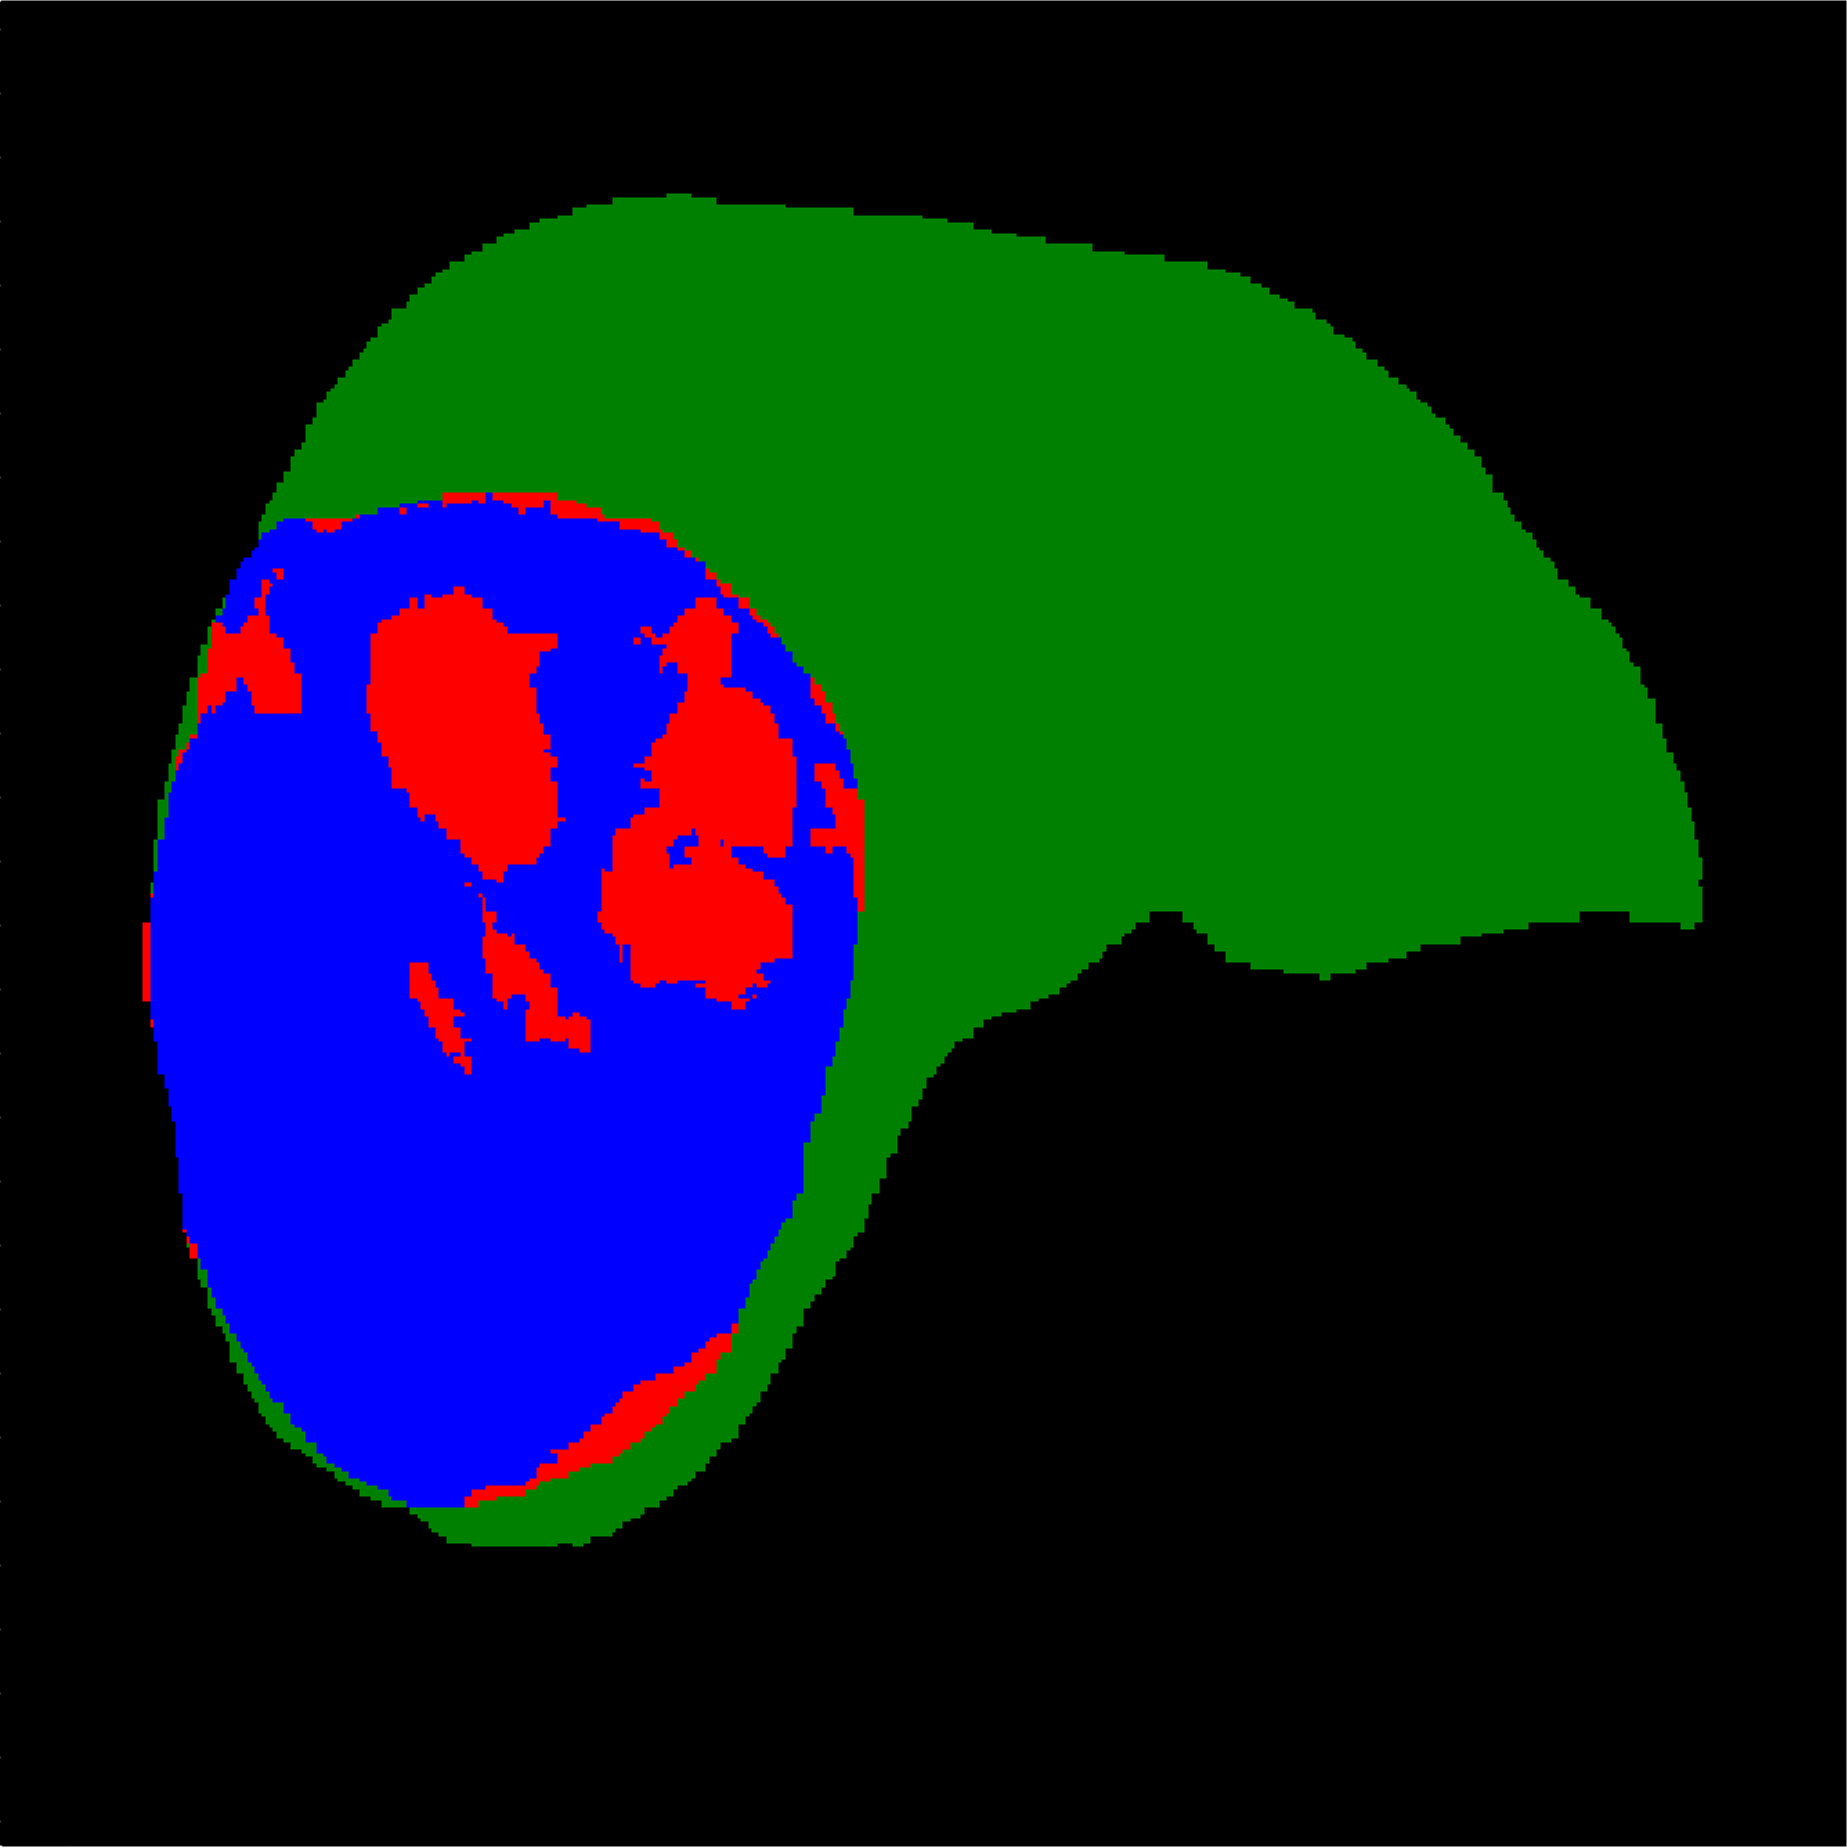
\includegraphics[width=\linewidth]{../SemanticSeg/images/5_2_gt_resized}
\end{minipage} \hspace{-0.3cm}
\begin{minipage}{4cm}
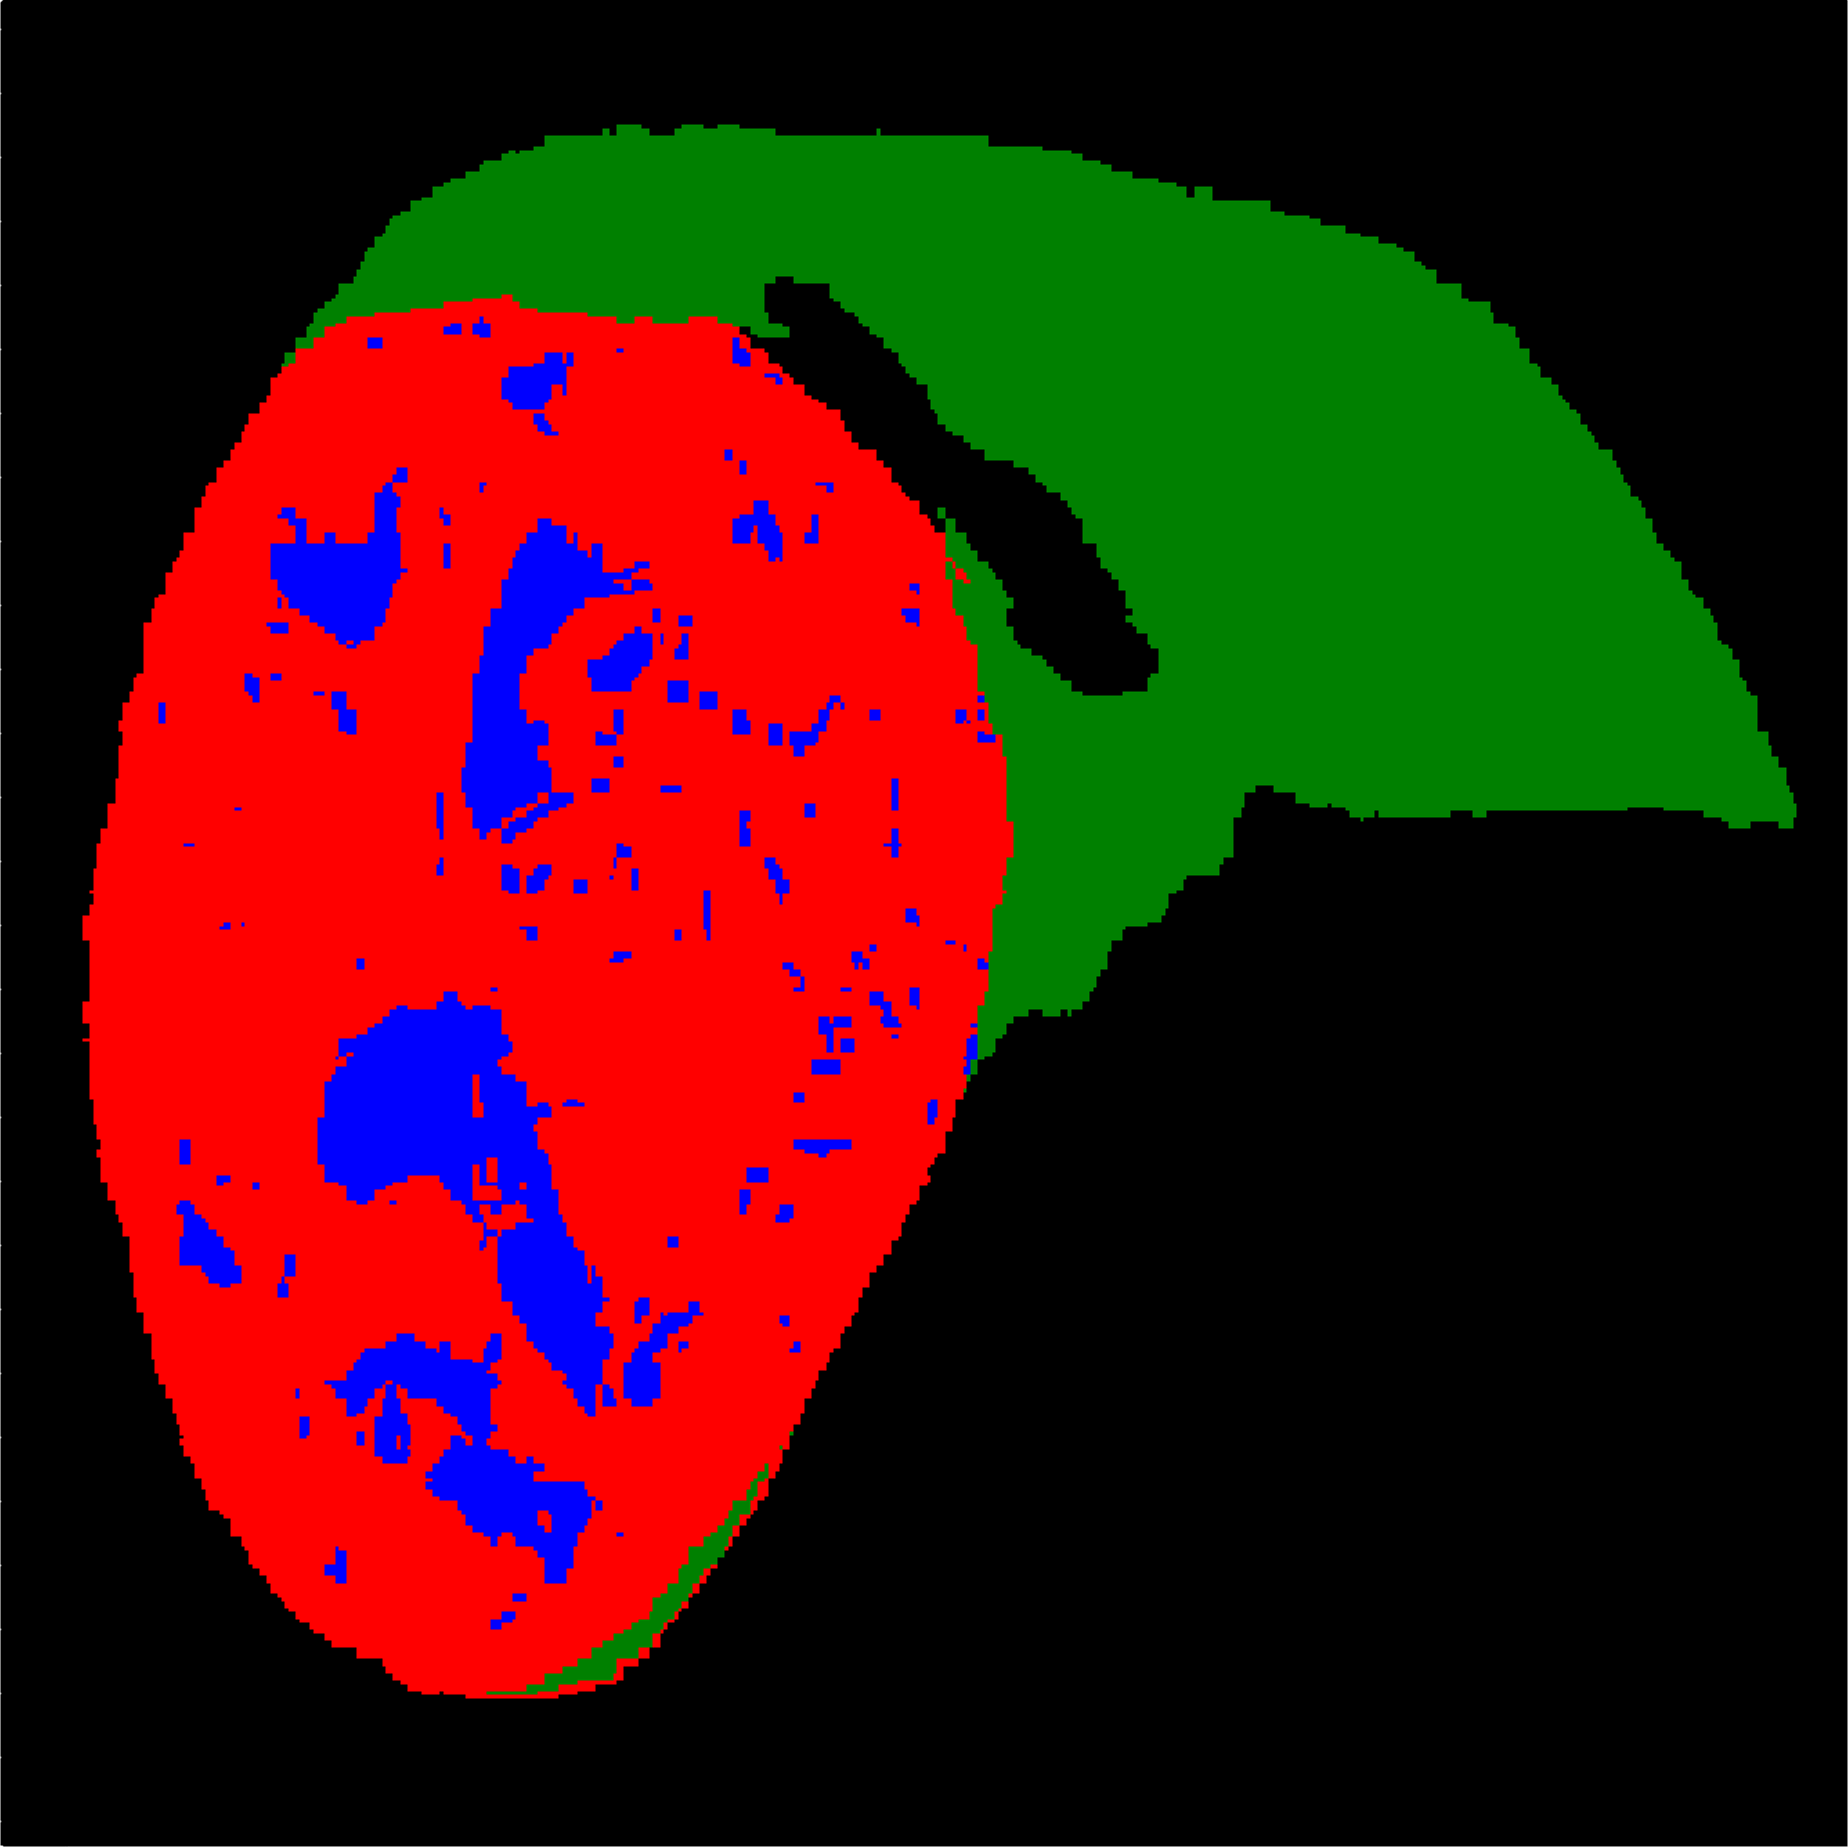
\includegraphics[width=\linewidth]{../SemanticSeg/images/5_8_gt_resized}
\end{minipage} 
\vspace{-0.2cm}
\begin{minipage}{4cm}
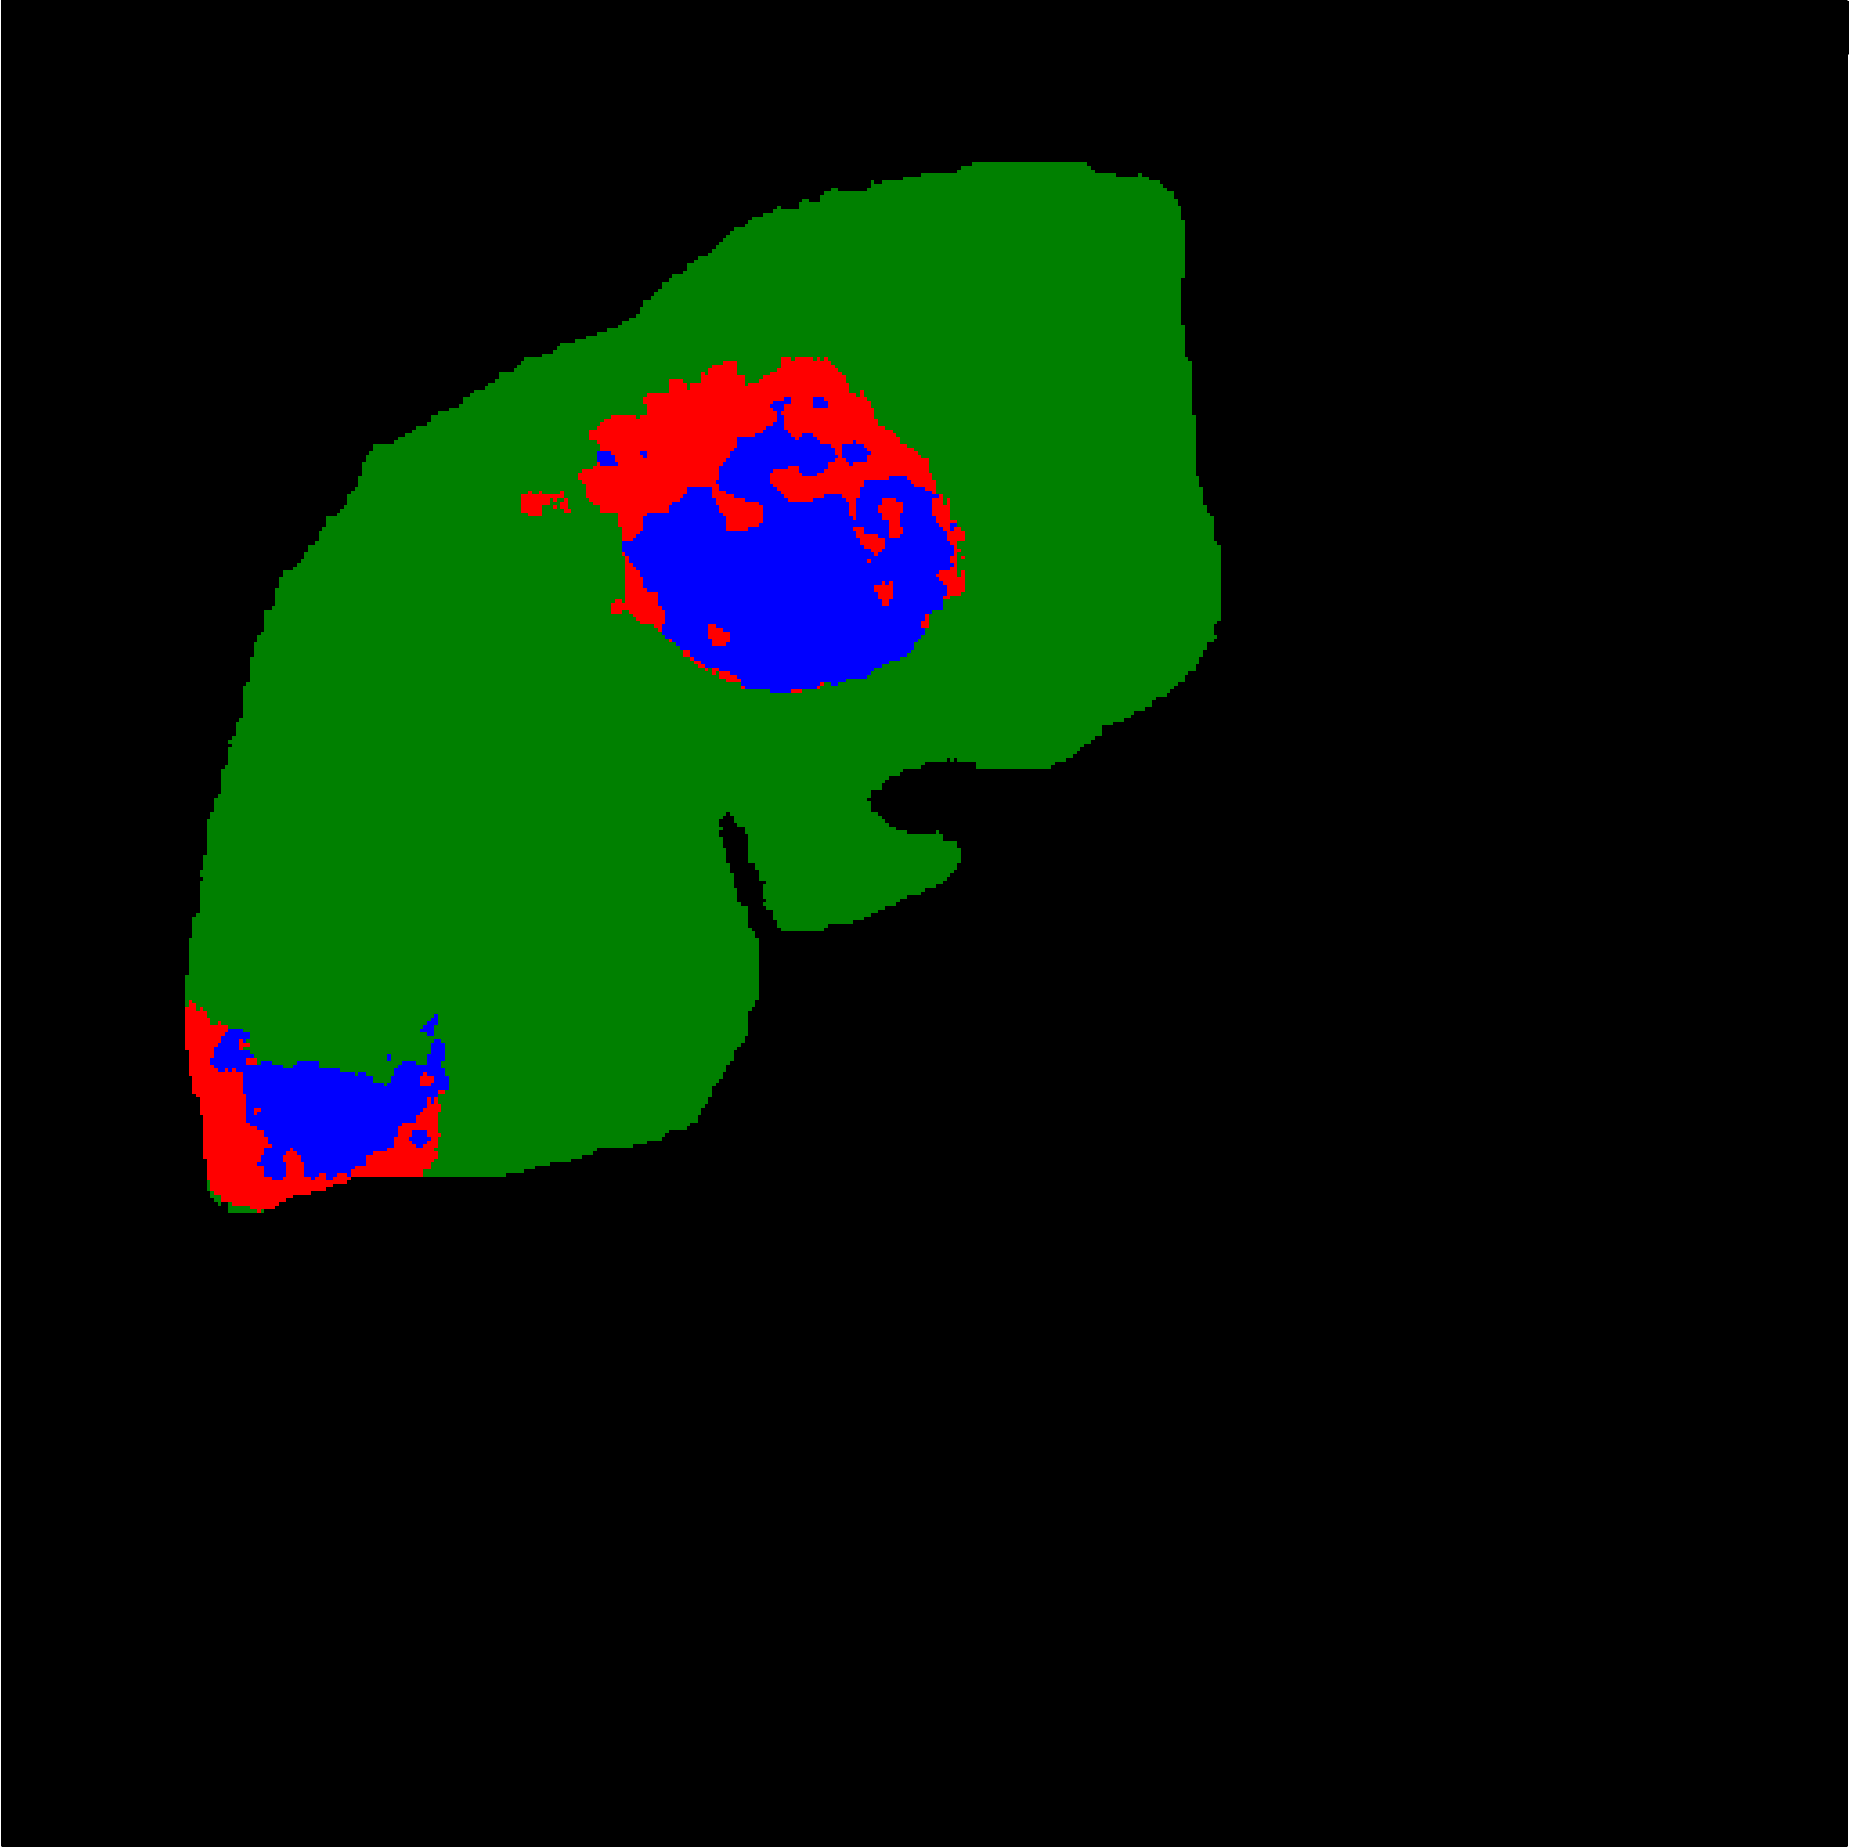
\includegraphics[width=\linewidth]{../SemanticSeg/images/1_21_FullDMP_resized}
\end{minipage} \hspace{-0.3cm}
\begin{minipage}{4cm}
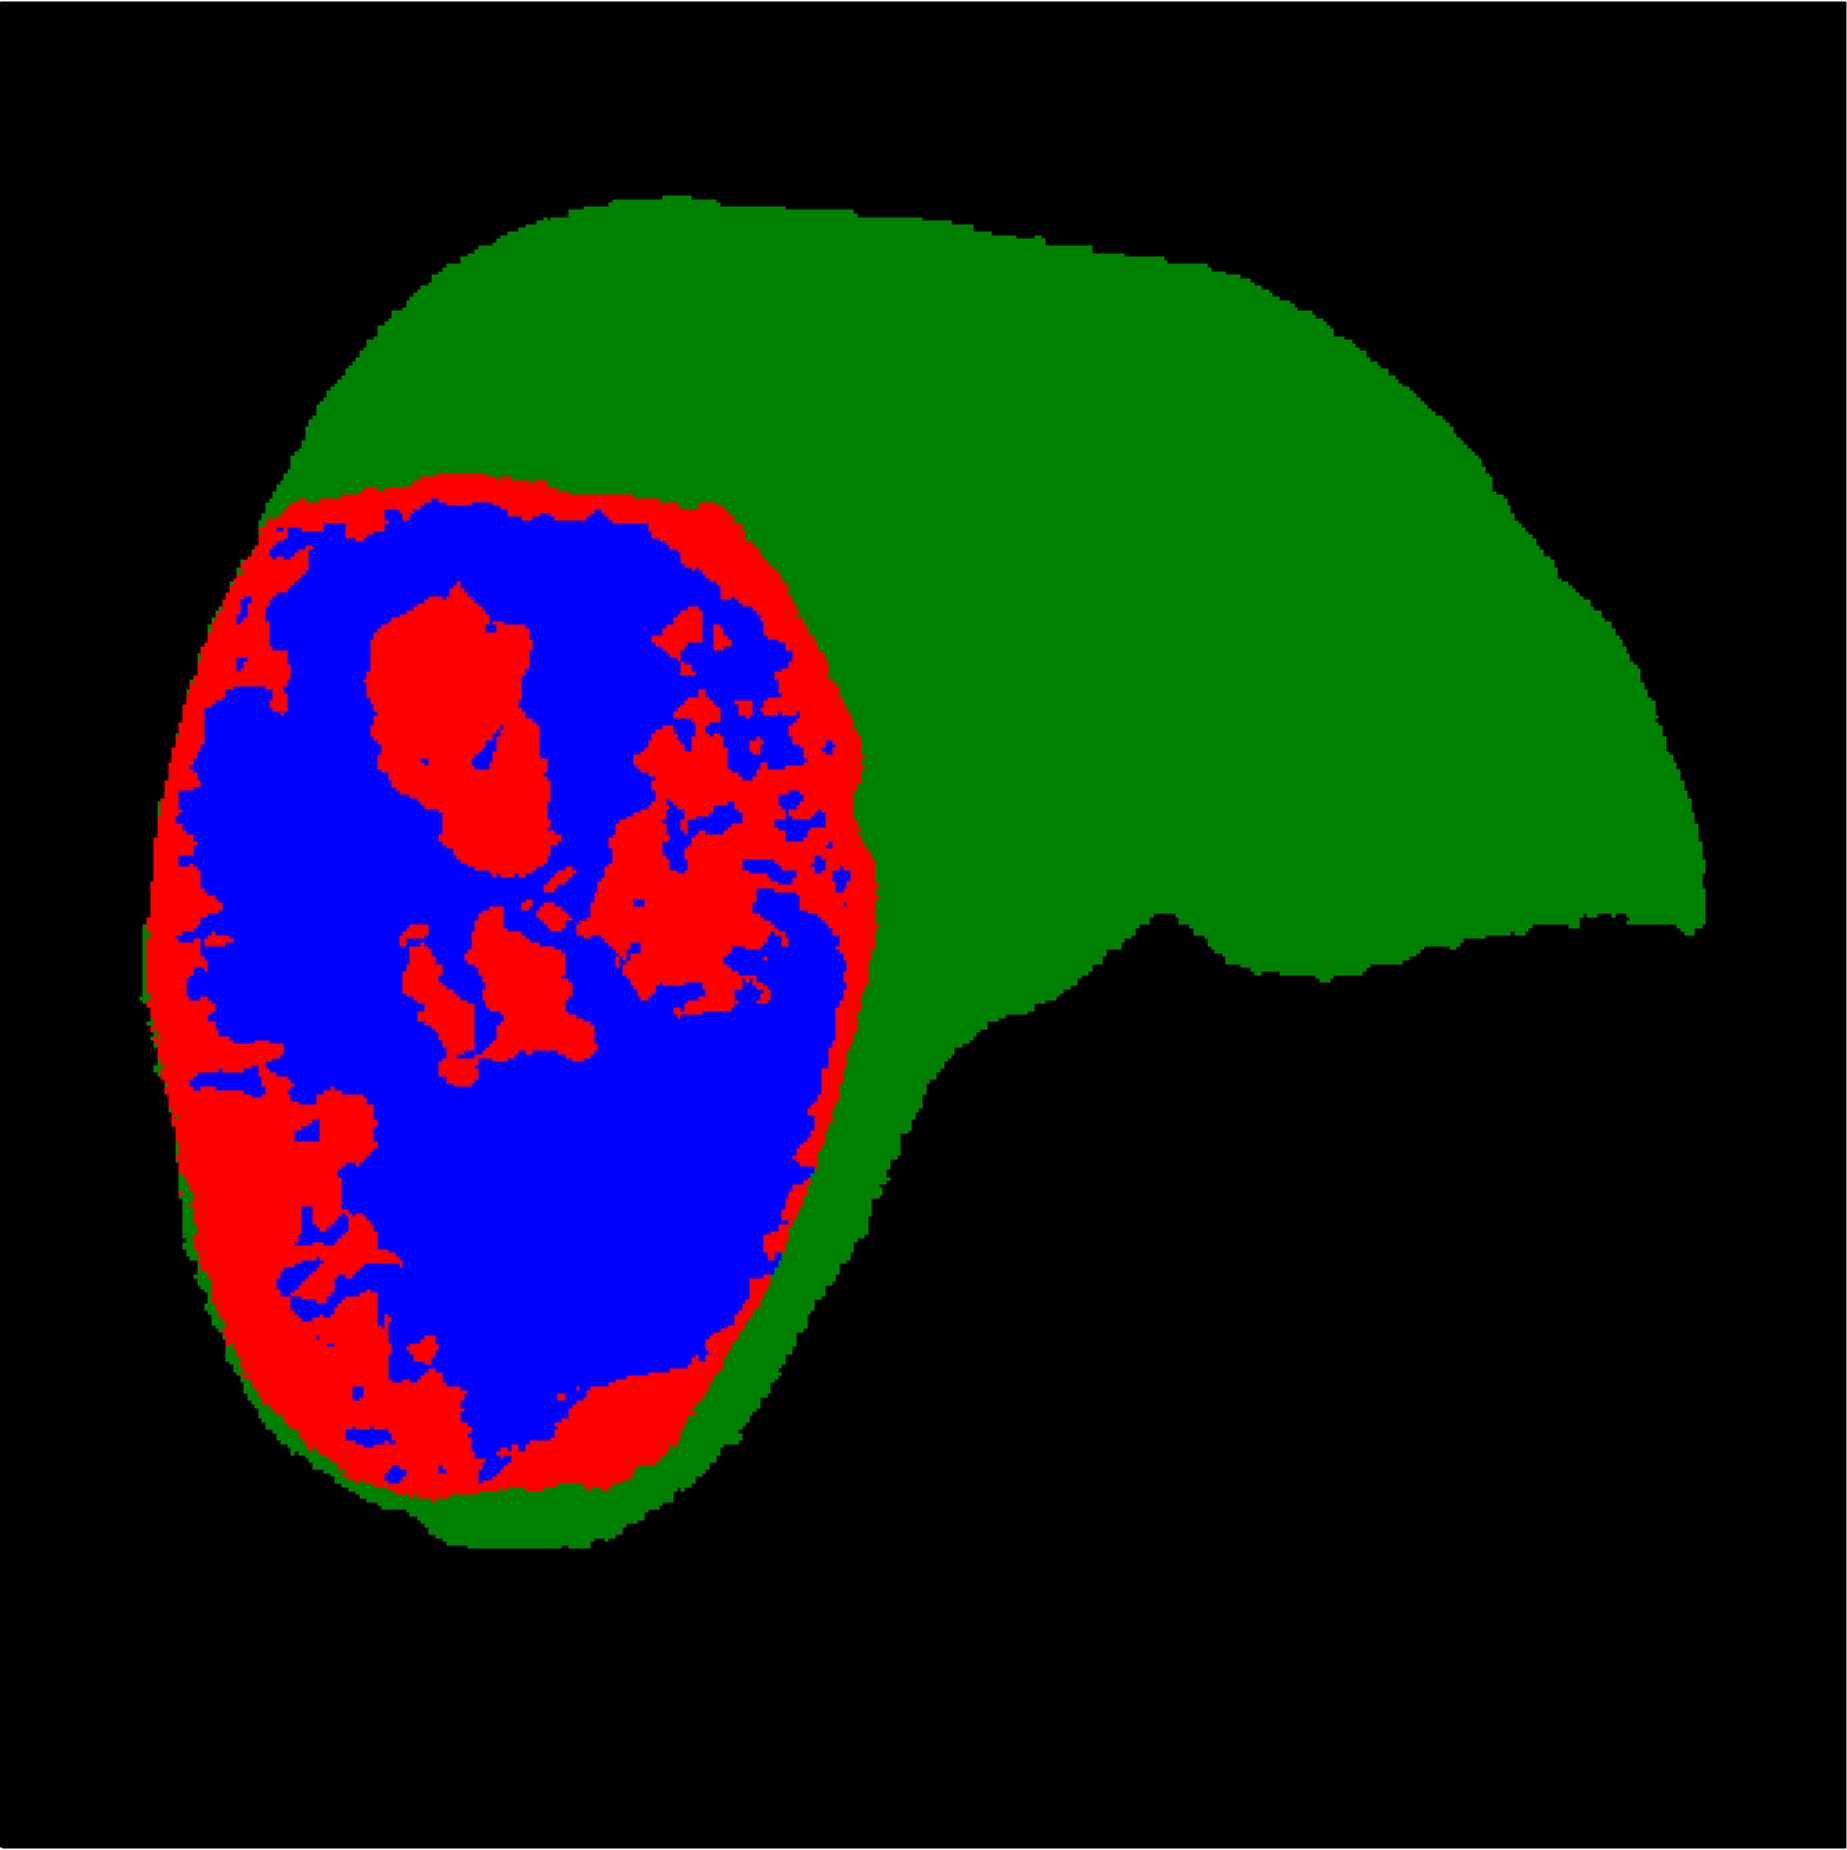
\includegraphics[width=\linewidth]{../SemanticSeg/images/5_2_FullDMP_resized}
\end{minipage} \hspace{-0.3cm}
\begin{minipage}{4cm}
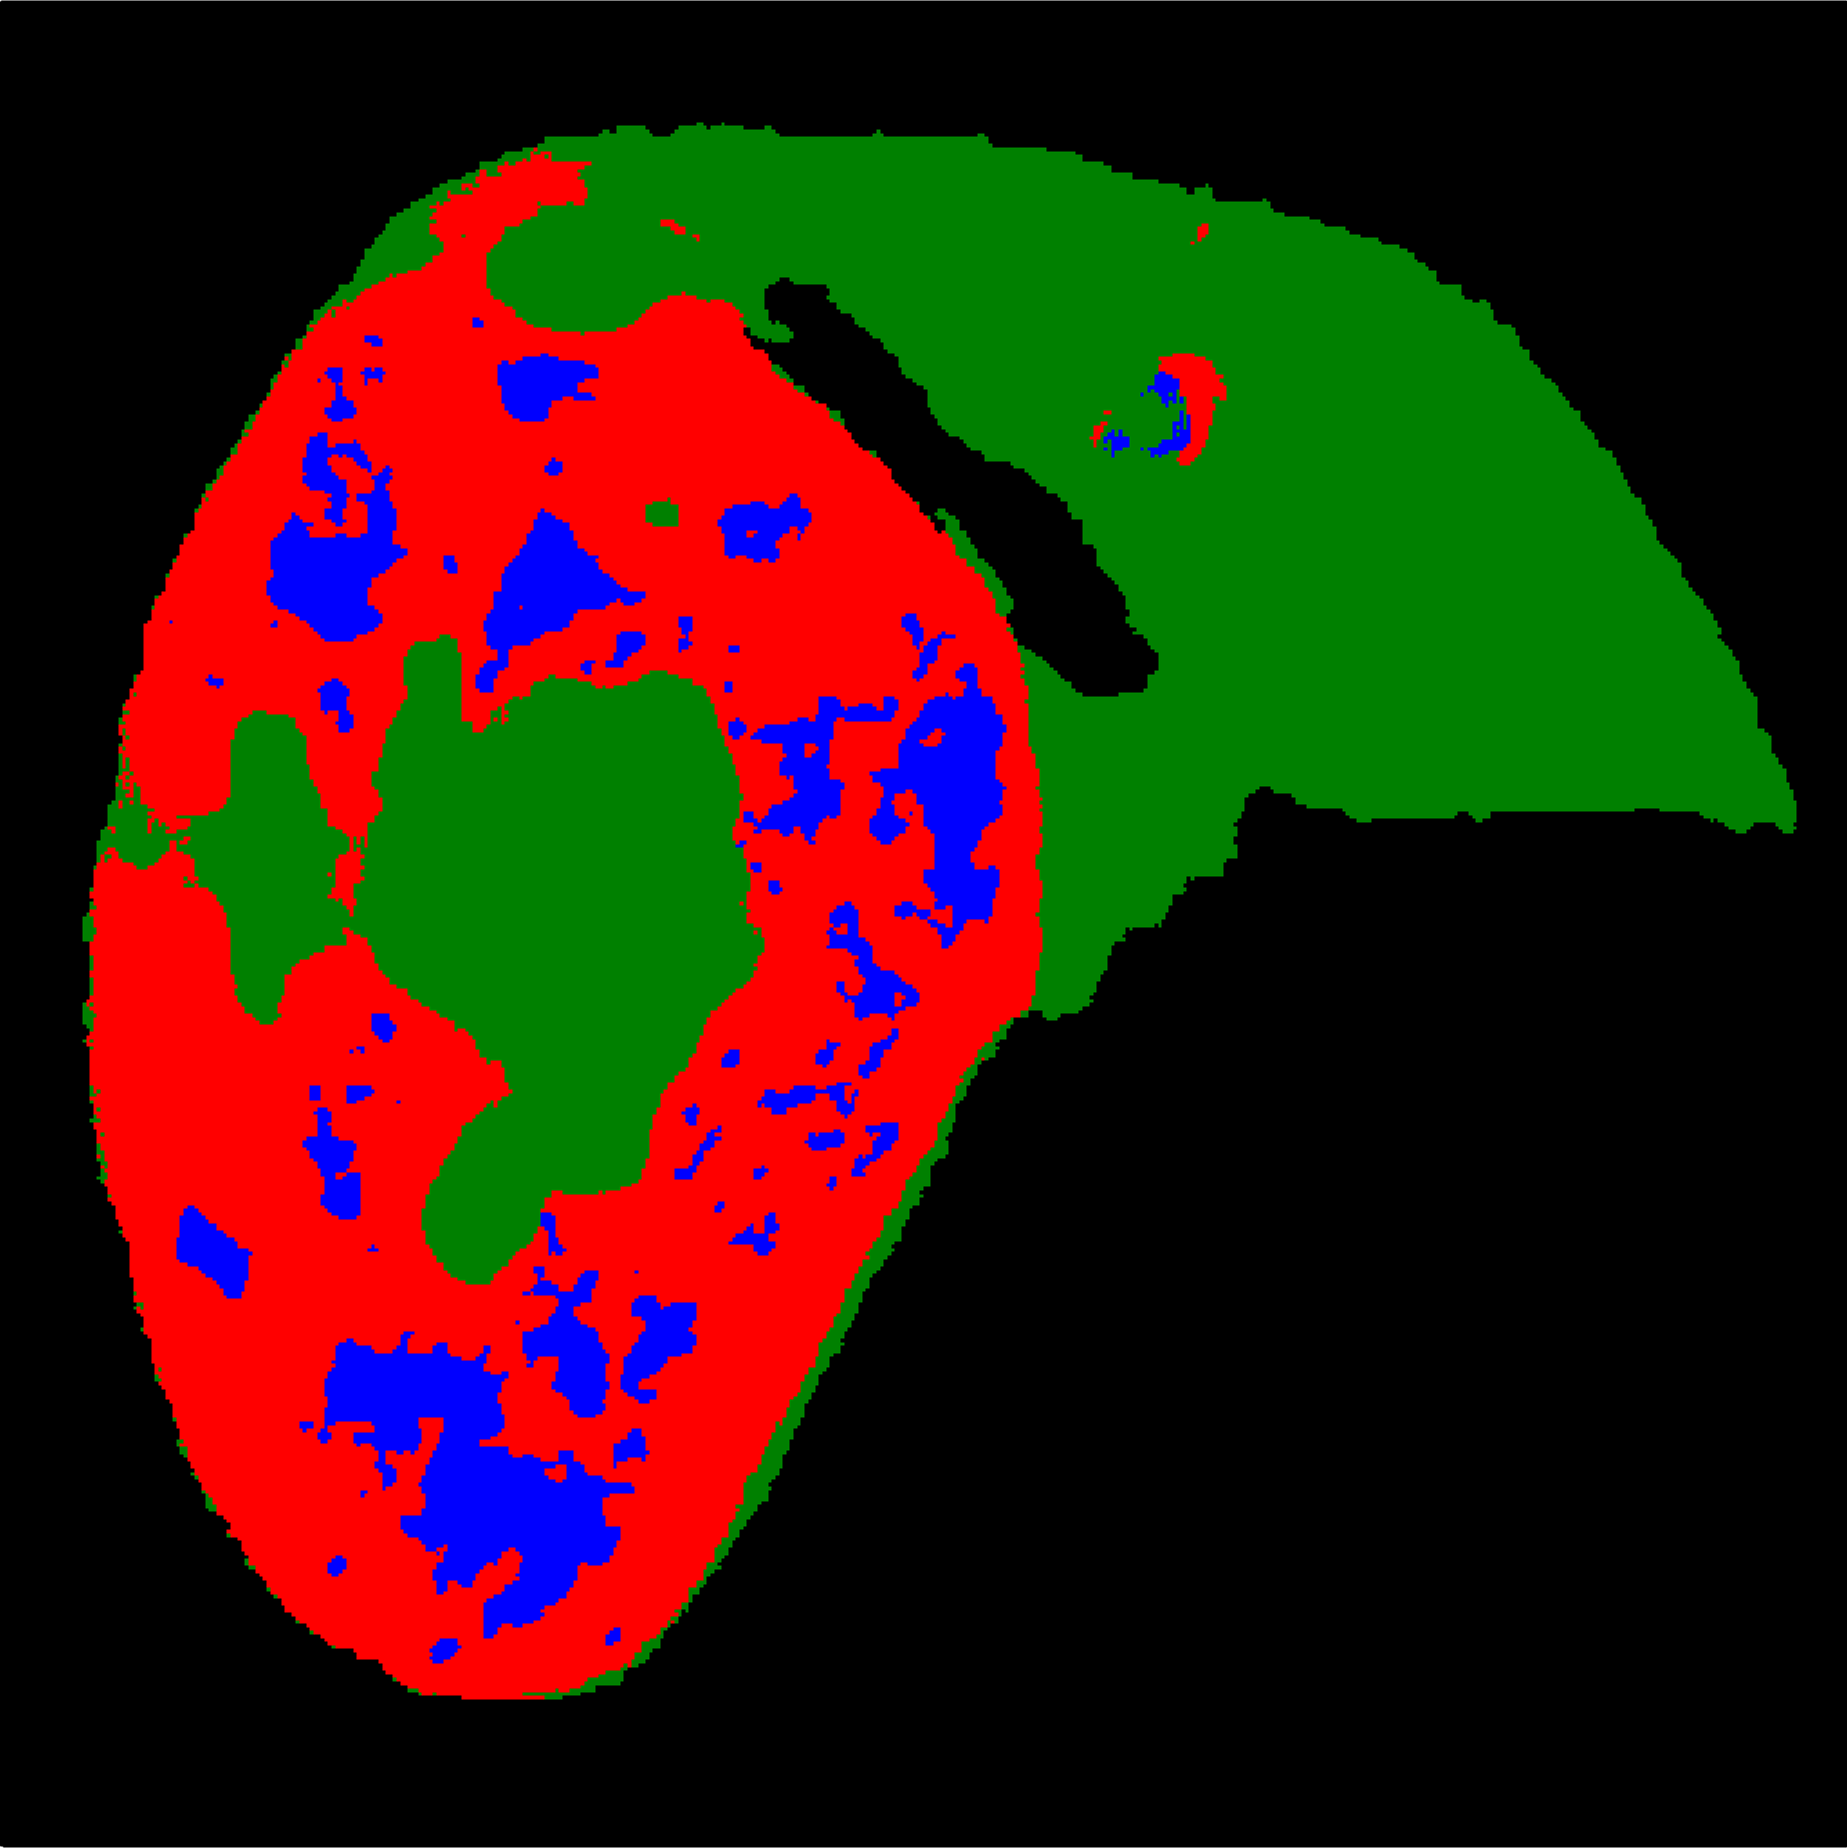
\includegraphics[width=\linewidth]{../SemanticSeg/images/5_8_FullDMP_resized}
\end{minipage} 
\vspace{-0.2cm}
\begin{minipage}{4cm}
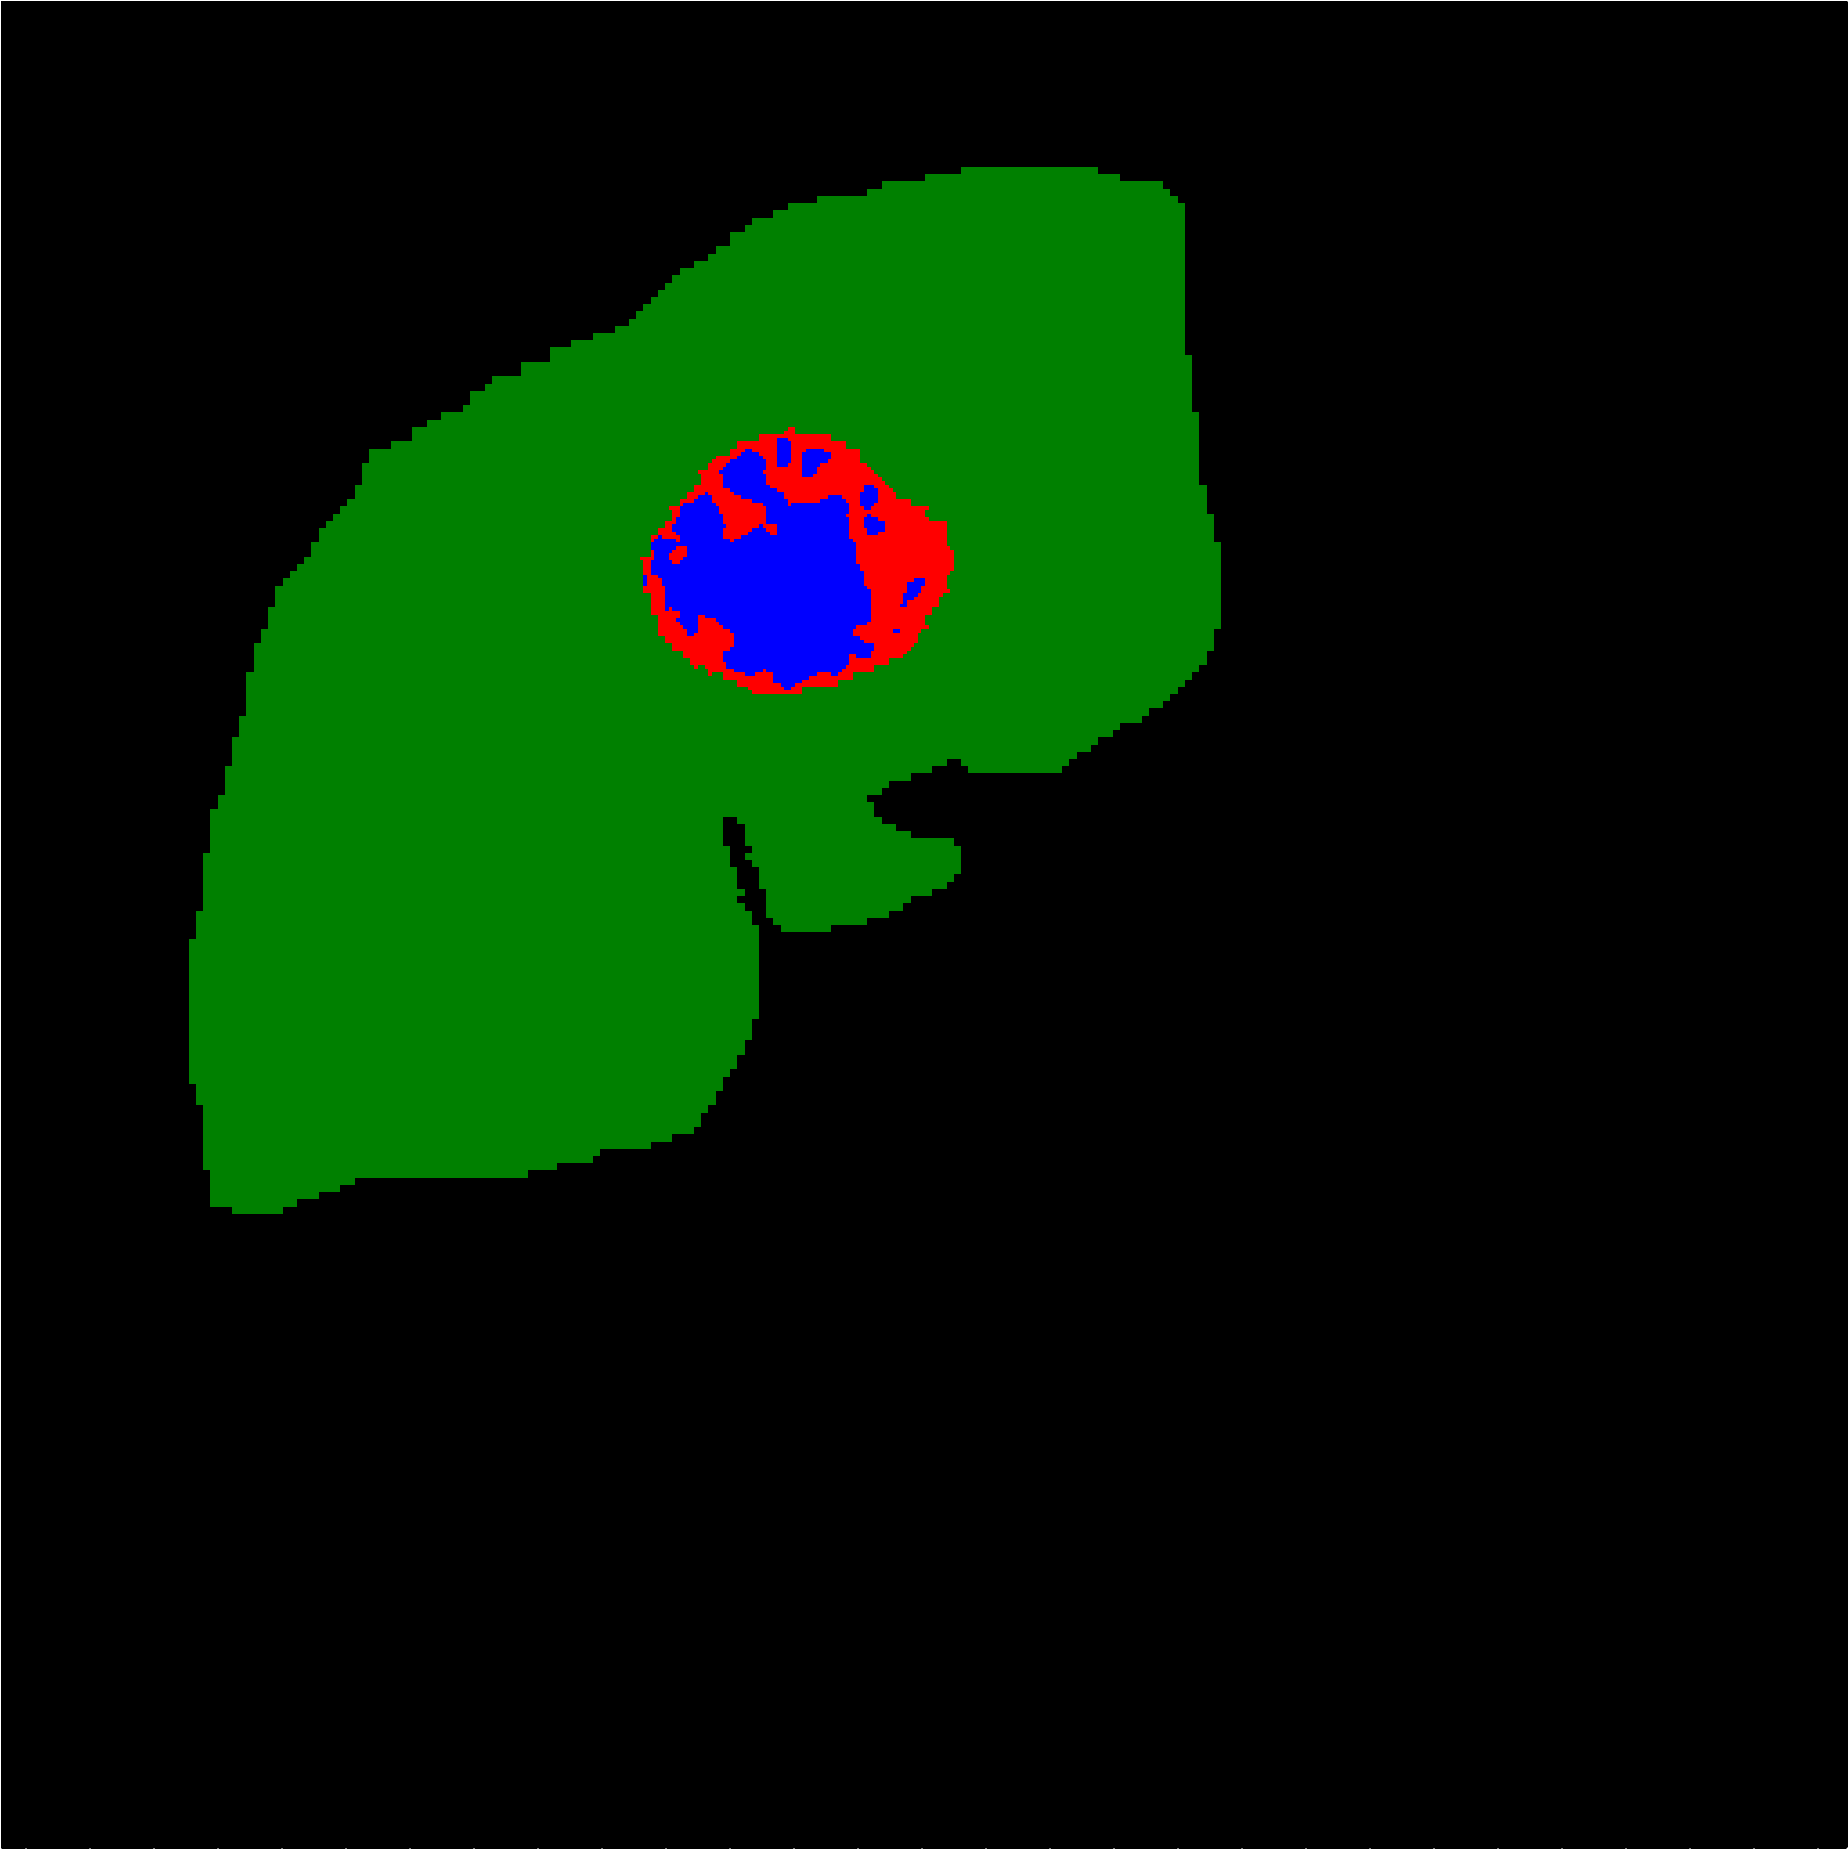
\includegraphics[width=\linewidth]{../SemanticSeg/images/1_21_Cascade_resized}
\end{minipage} \hspace{-0.3cm}
\begin{minipage}{4cm}
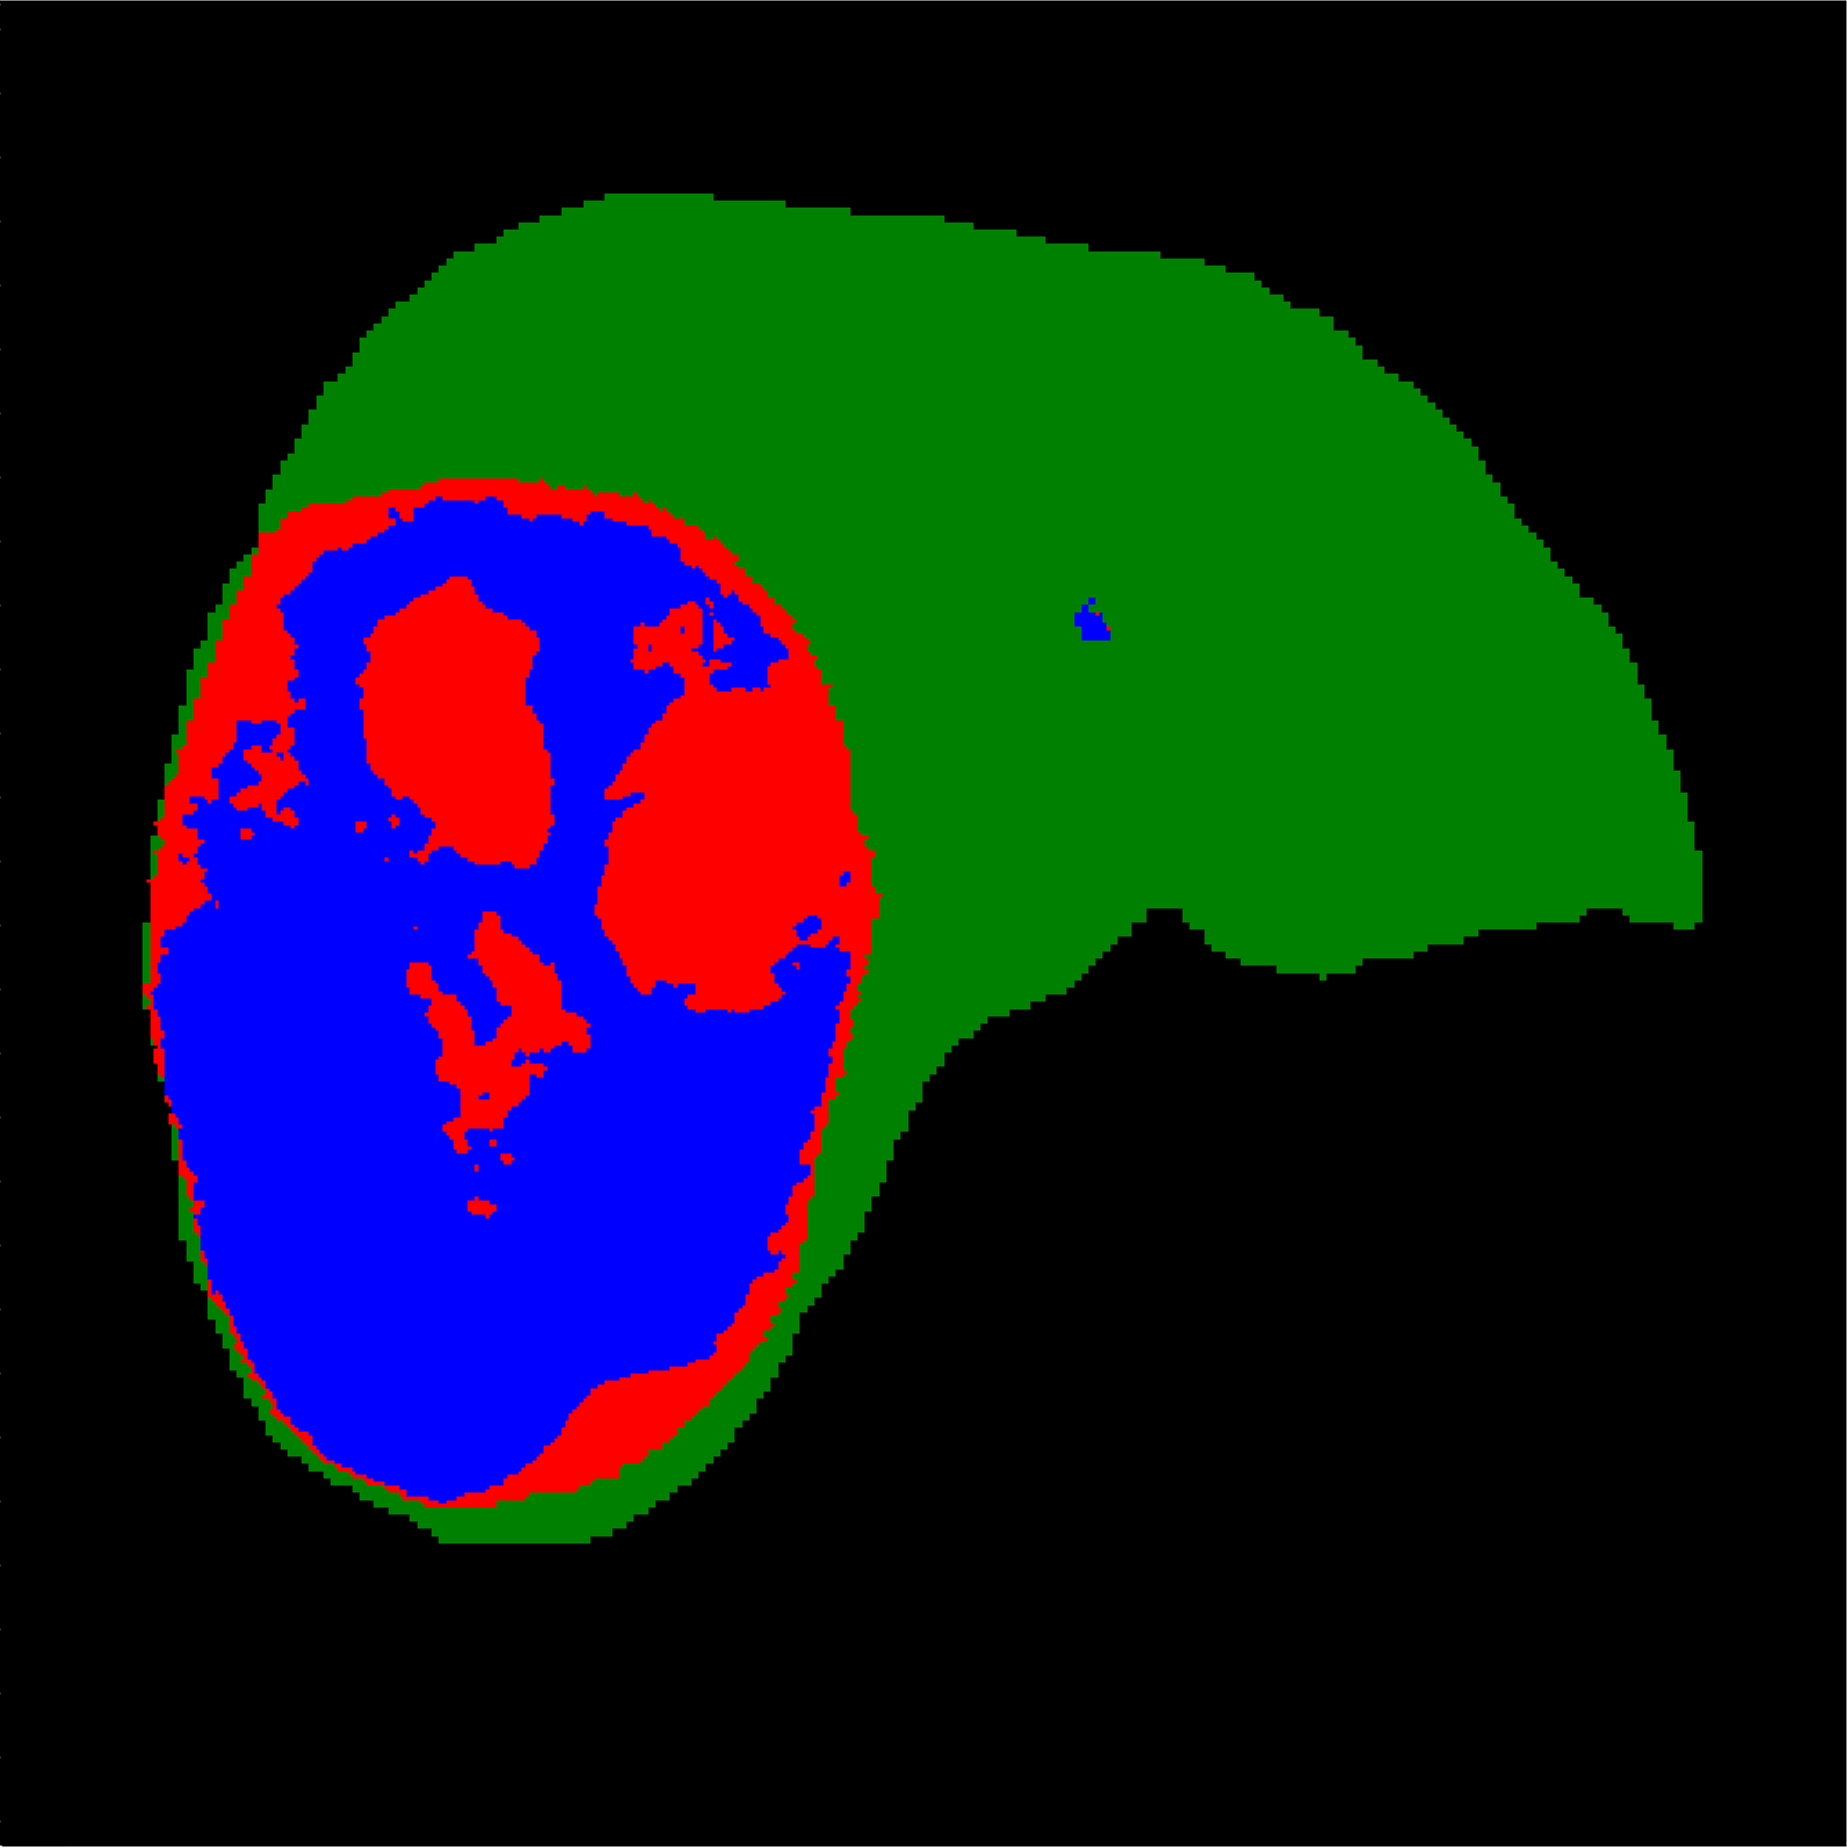
\includegraphics[width=\linewidth]{../SemanticSeg/images/5_2_Cascade_resized}
\end{minipage} \hspace{-0.3cm}
\begin{minipage}{4cm}
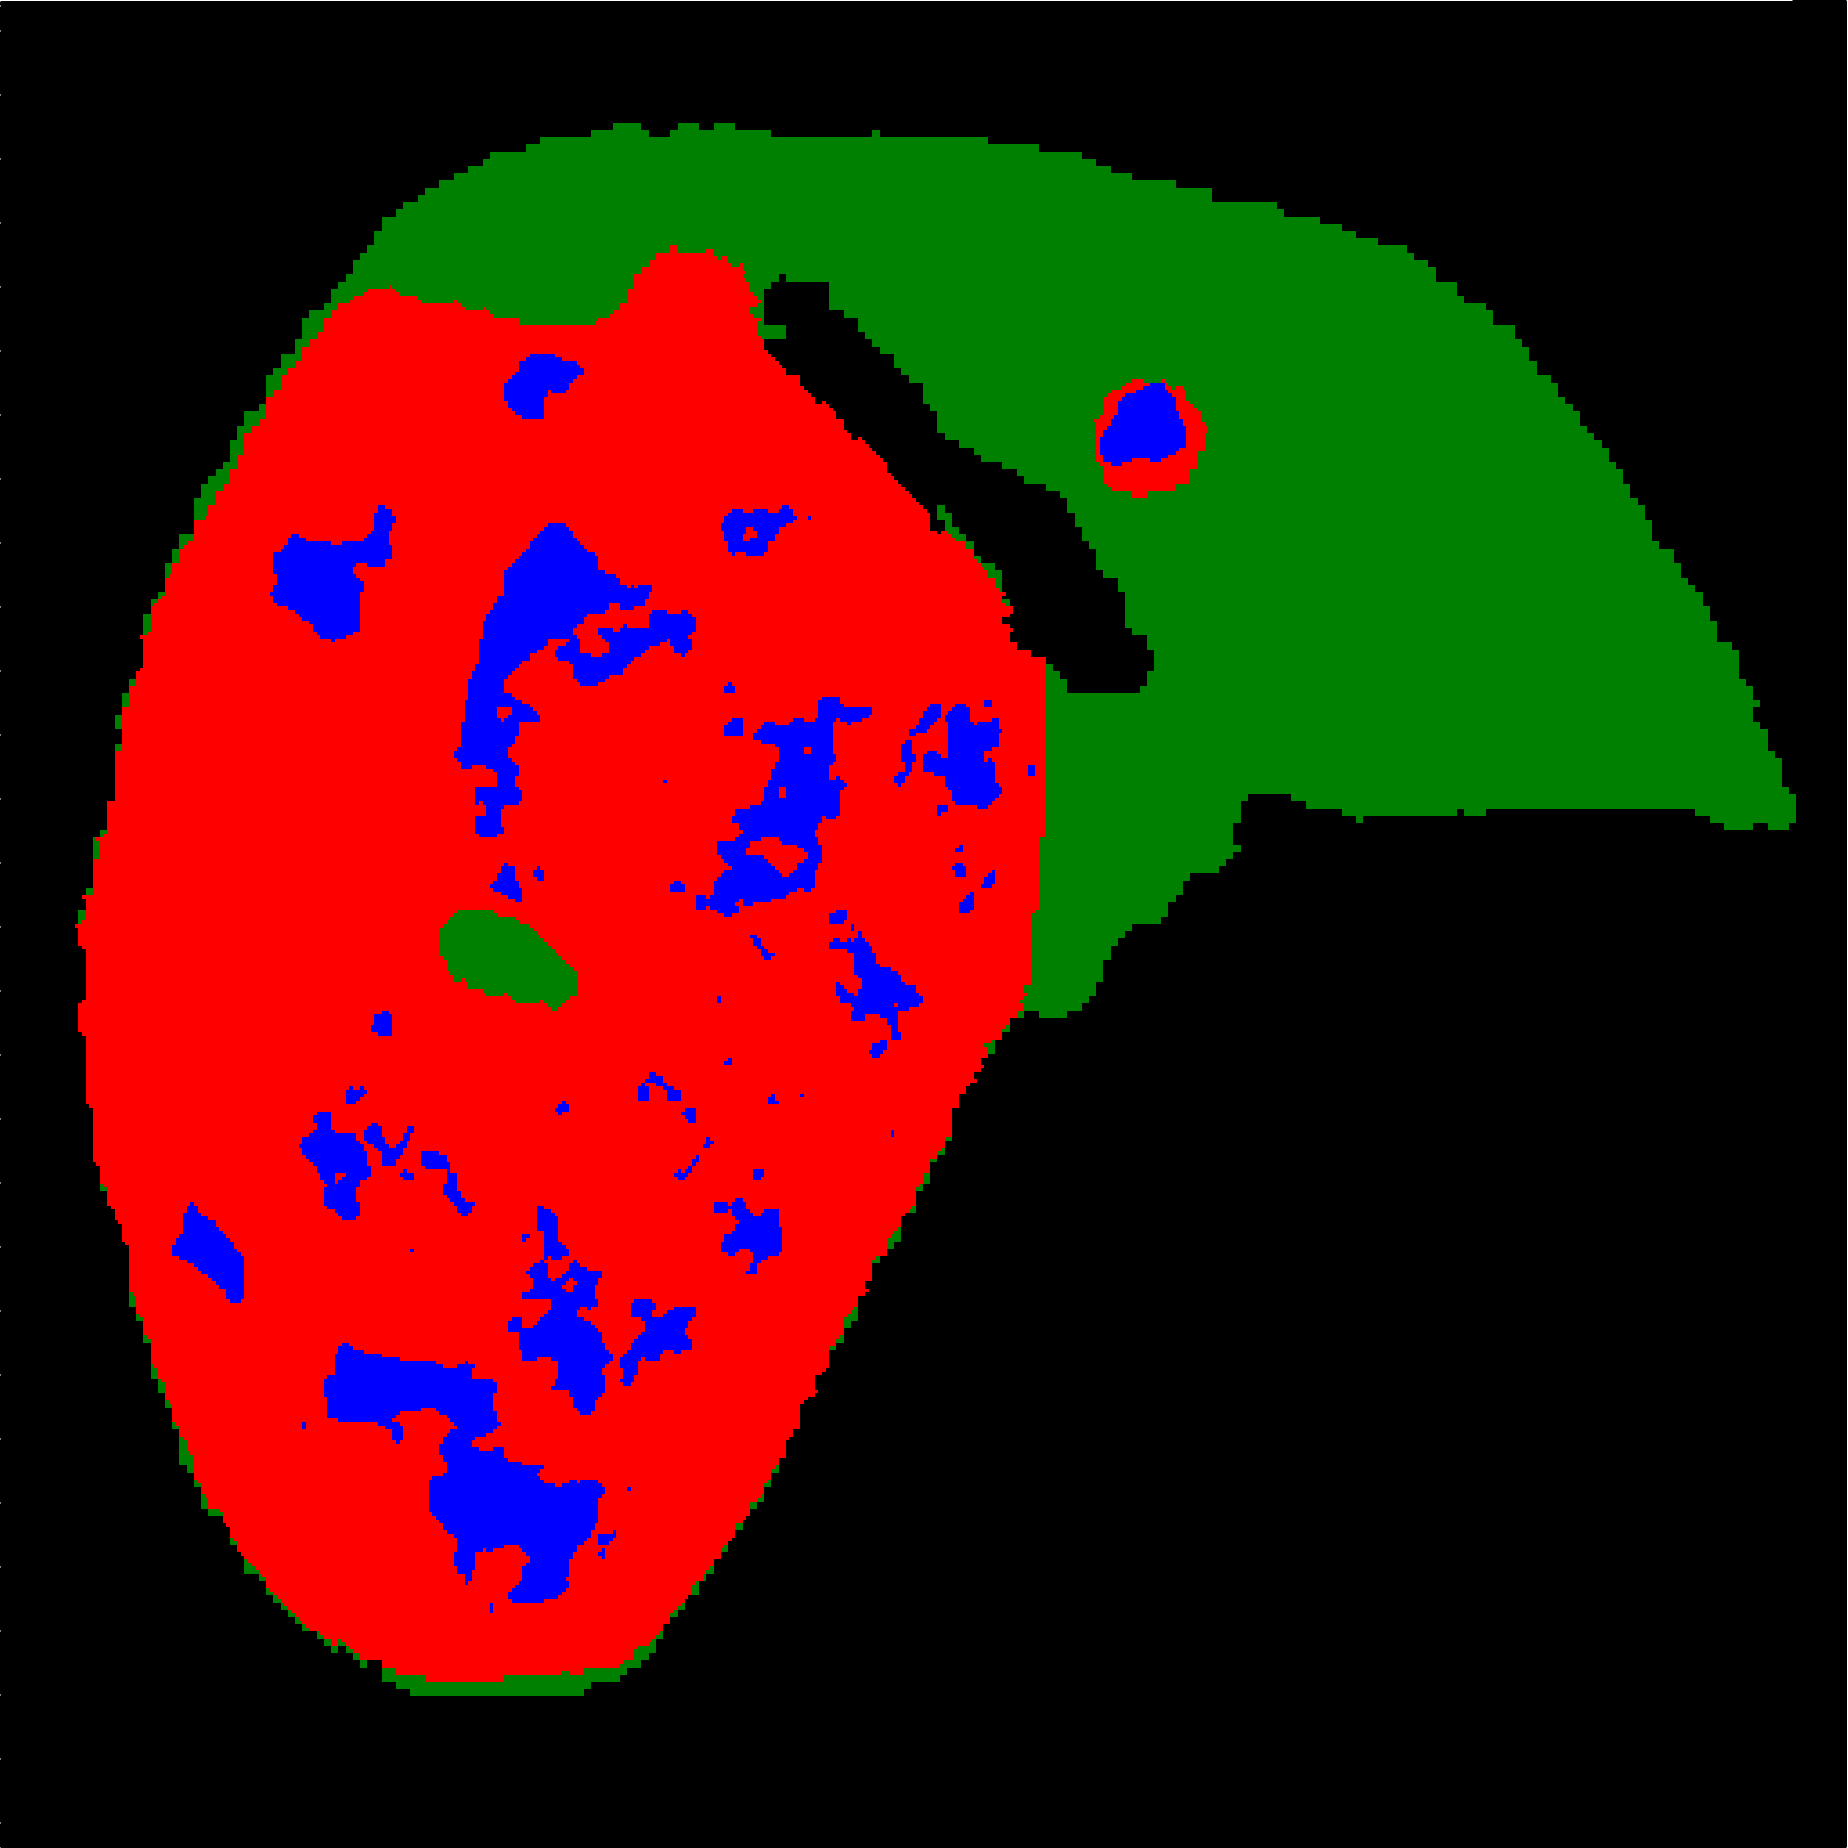
\includegraphics[width=\linewidth]{../SemanticSeg/images/5_8_Cascade_resized}
\end{minipage} 
\caption{From top to bottom : Raw images with HU values inside the liver, Ground truth, \pplfont{DMP-Full} segmentation, Cascaded DMP segmentation}
\label{CompareFullCascade}
\end{figure}


We finally combined the \pplfont{DMP-Liver}, the \pplfont{DMP-Lesion} and \pplfont{DMP-Necrosis} networks in a cascaded fashion, as described in the figure \ref{CARS_Cascade}. This allowed us to perform a fully automatic segmentation of the raw (unmasked) \ac{ct} images. We reached average slice-wise \ac{dsc}s of 78.3 $\pm$ 22.1 for the segmentation of the parenchyma, 50.6 $\pm$ 24.6  for the segmentation of the active part, and 68.1 $\pm$ 23.2 for the necrotic part of the lesions. We also provided a necrosis rate per patient with a mean error of 15.9\% when compared to expert necrosis rate estimation \footnote{Here the estimation is performed on the raw images in an automatic fashion}. Examples of fully automatic segmentation results are given in figure \ref{FullAutoSeg}.

\begin{figure}[!ht]
   \centering
\begin{minipage}{4cm}
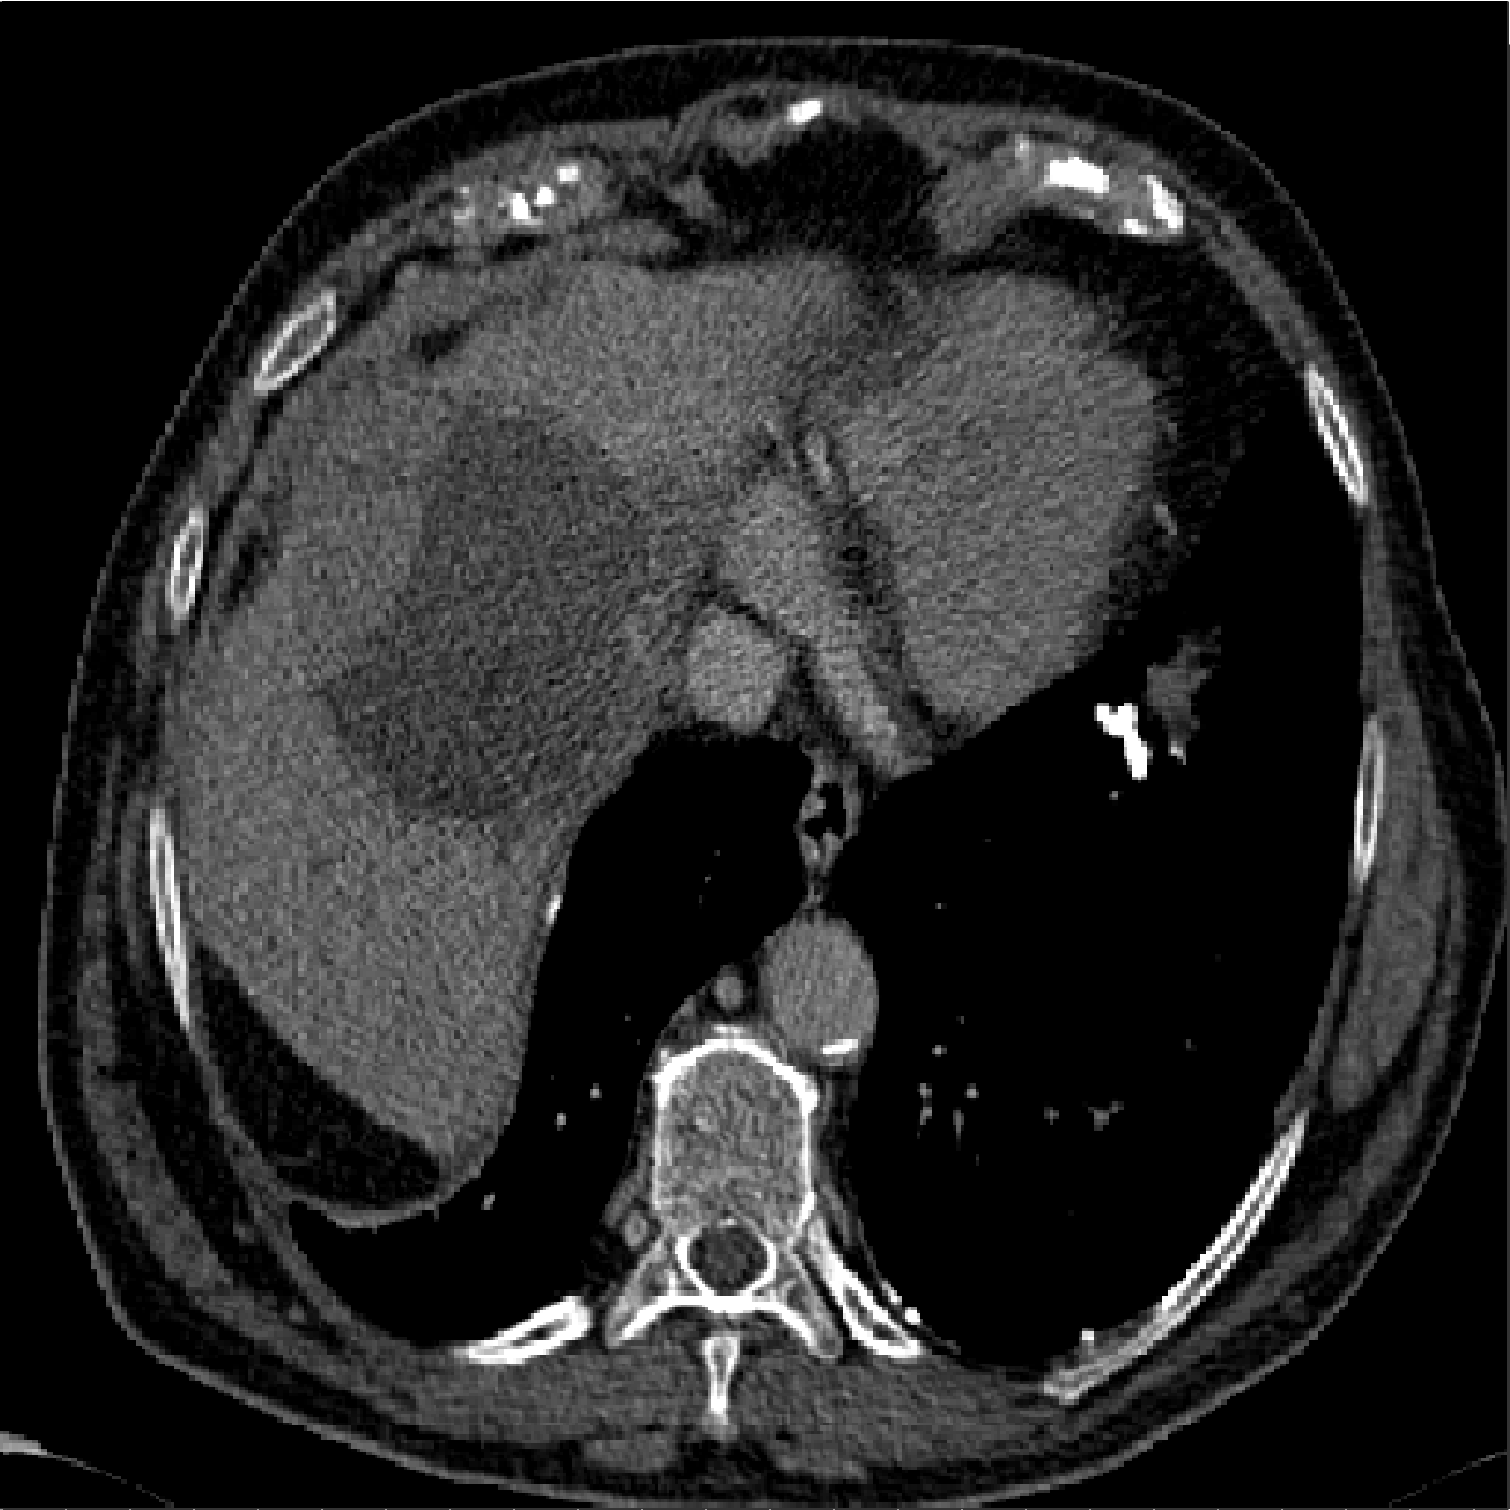
\includegraphics[width=\linewidth]{../SemanticSeg/images/1_7_raw_new_resized}
\end{minipage} \hspace{-0.3cm}
\begin{minipage}{4cm}
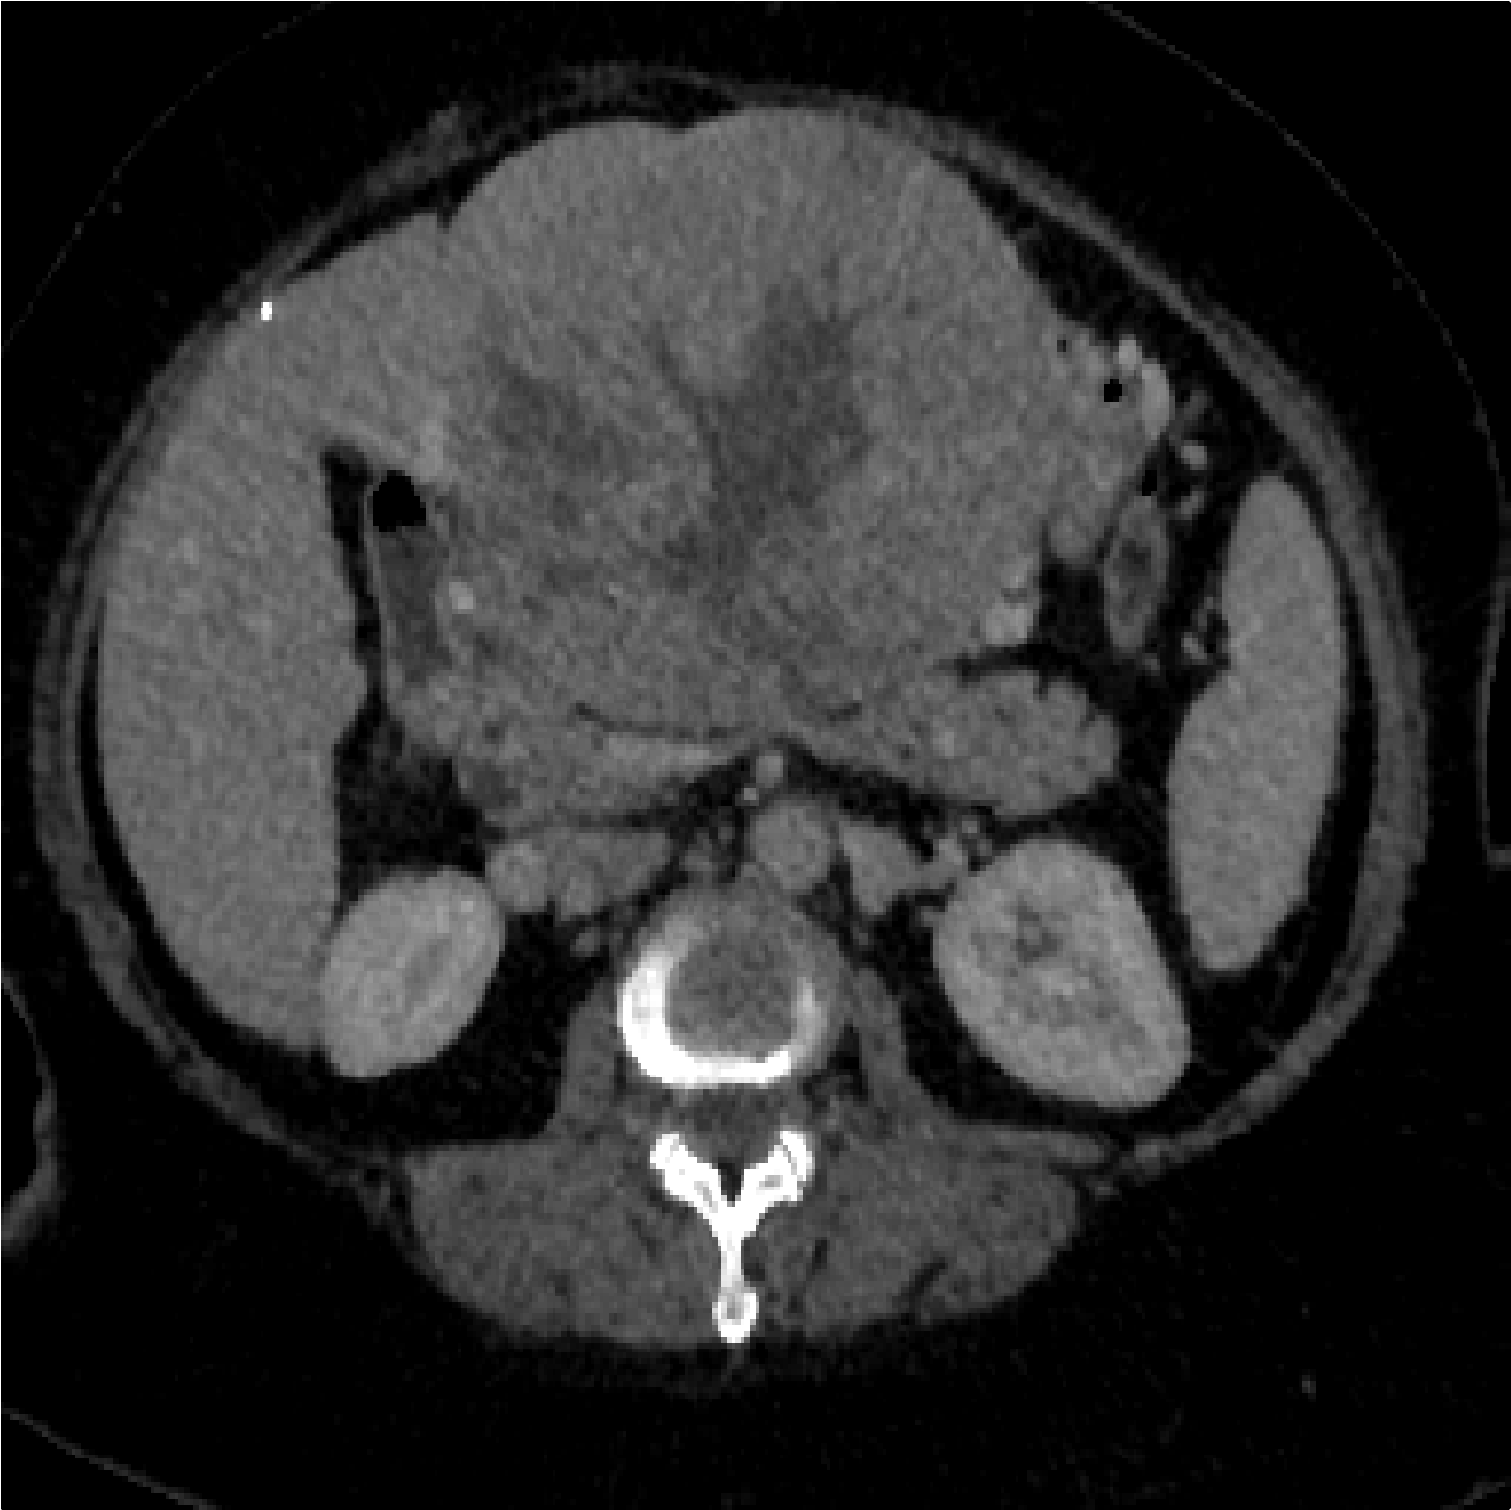
\includegraphics[width=\linewidth]{../SemanticSeg/images/2_3_raw_resized}
\end{minipage} \hspace{-0.3cm}
\begin{minipage}{4cm}
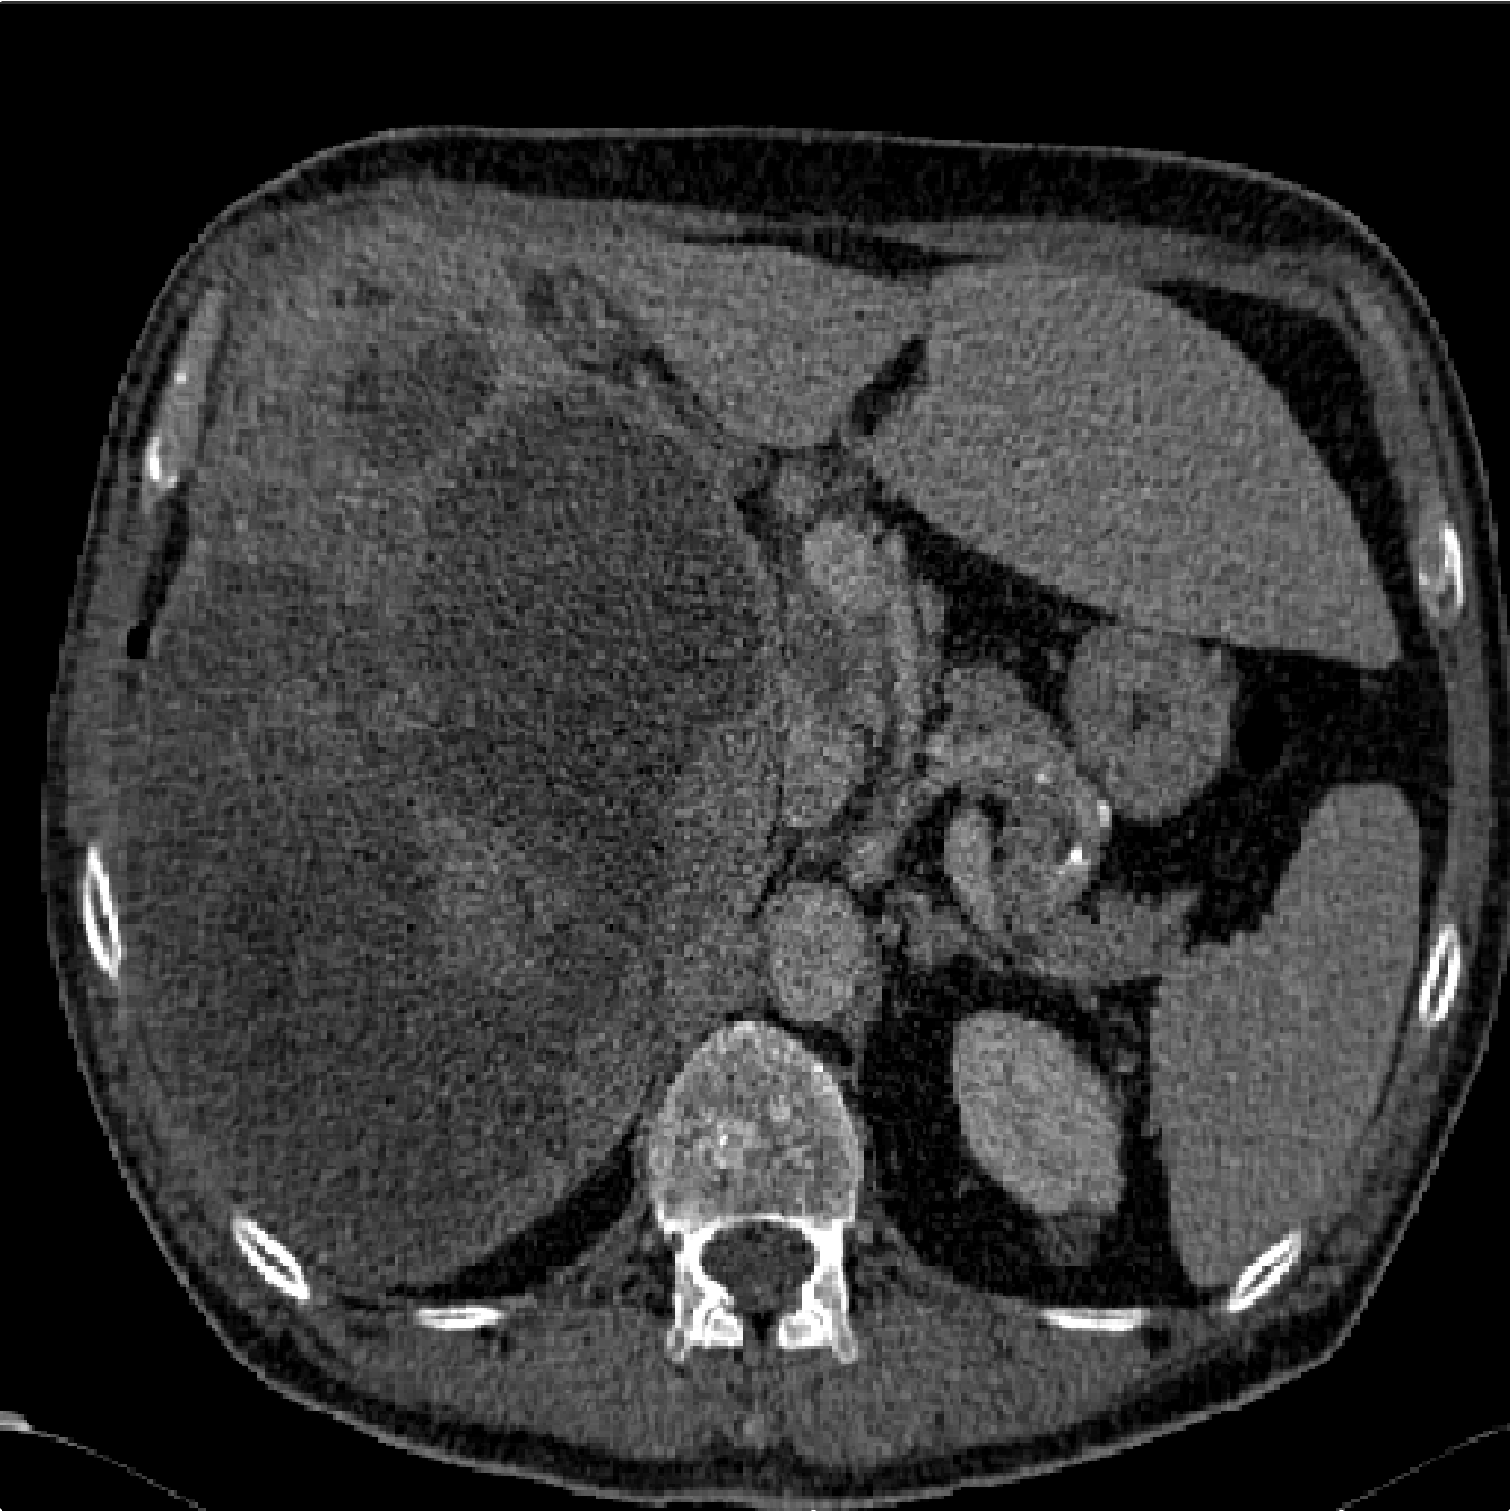
\includegraphics[width=\linewidth]{../SemanticSeg/images/5_4_raw_resized}
\end{minipage}
\vspace{-0.2cm}
\begin{minipage}{4cm}
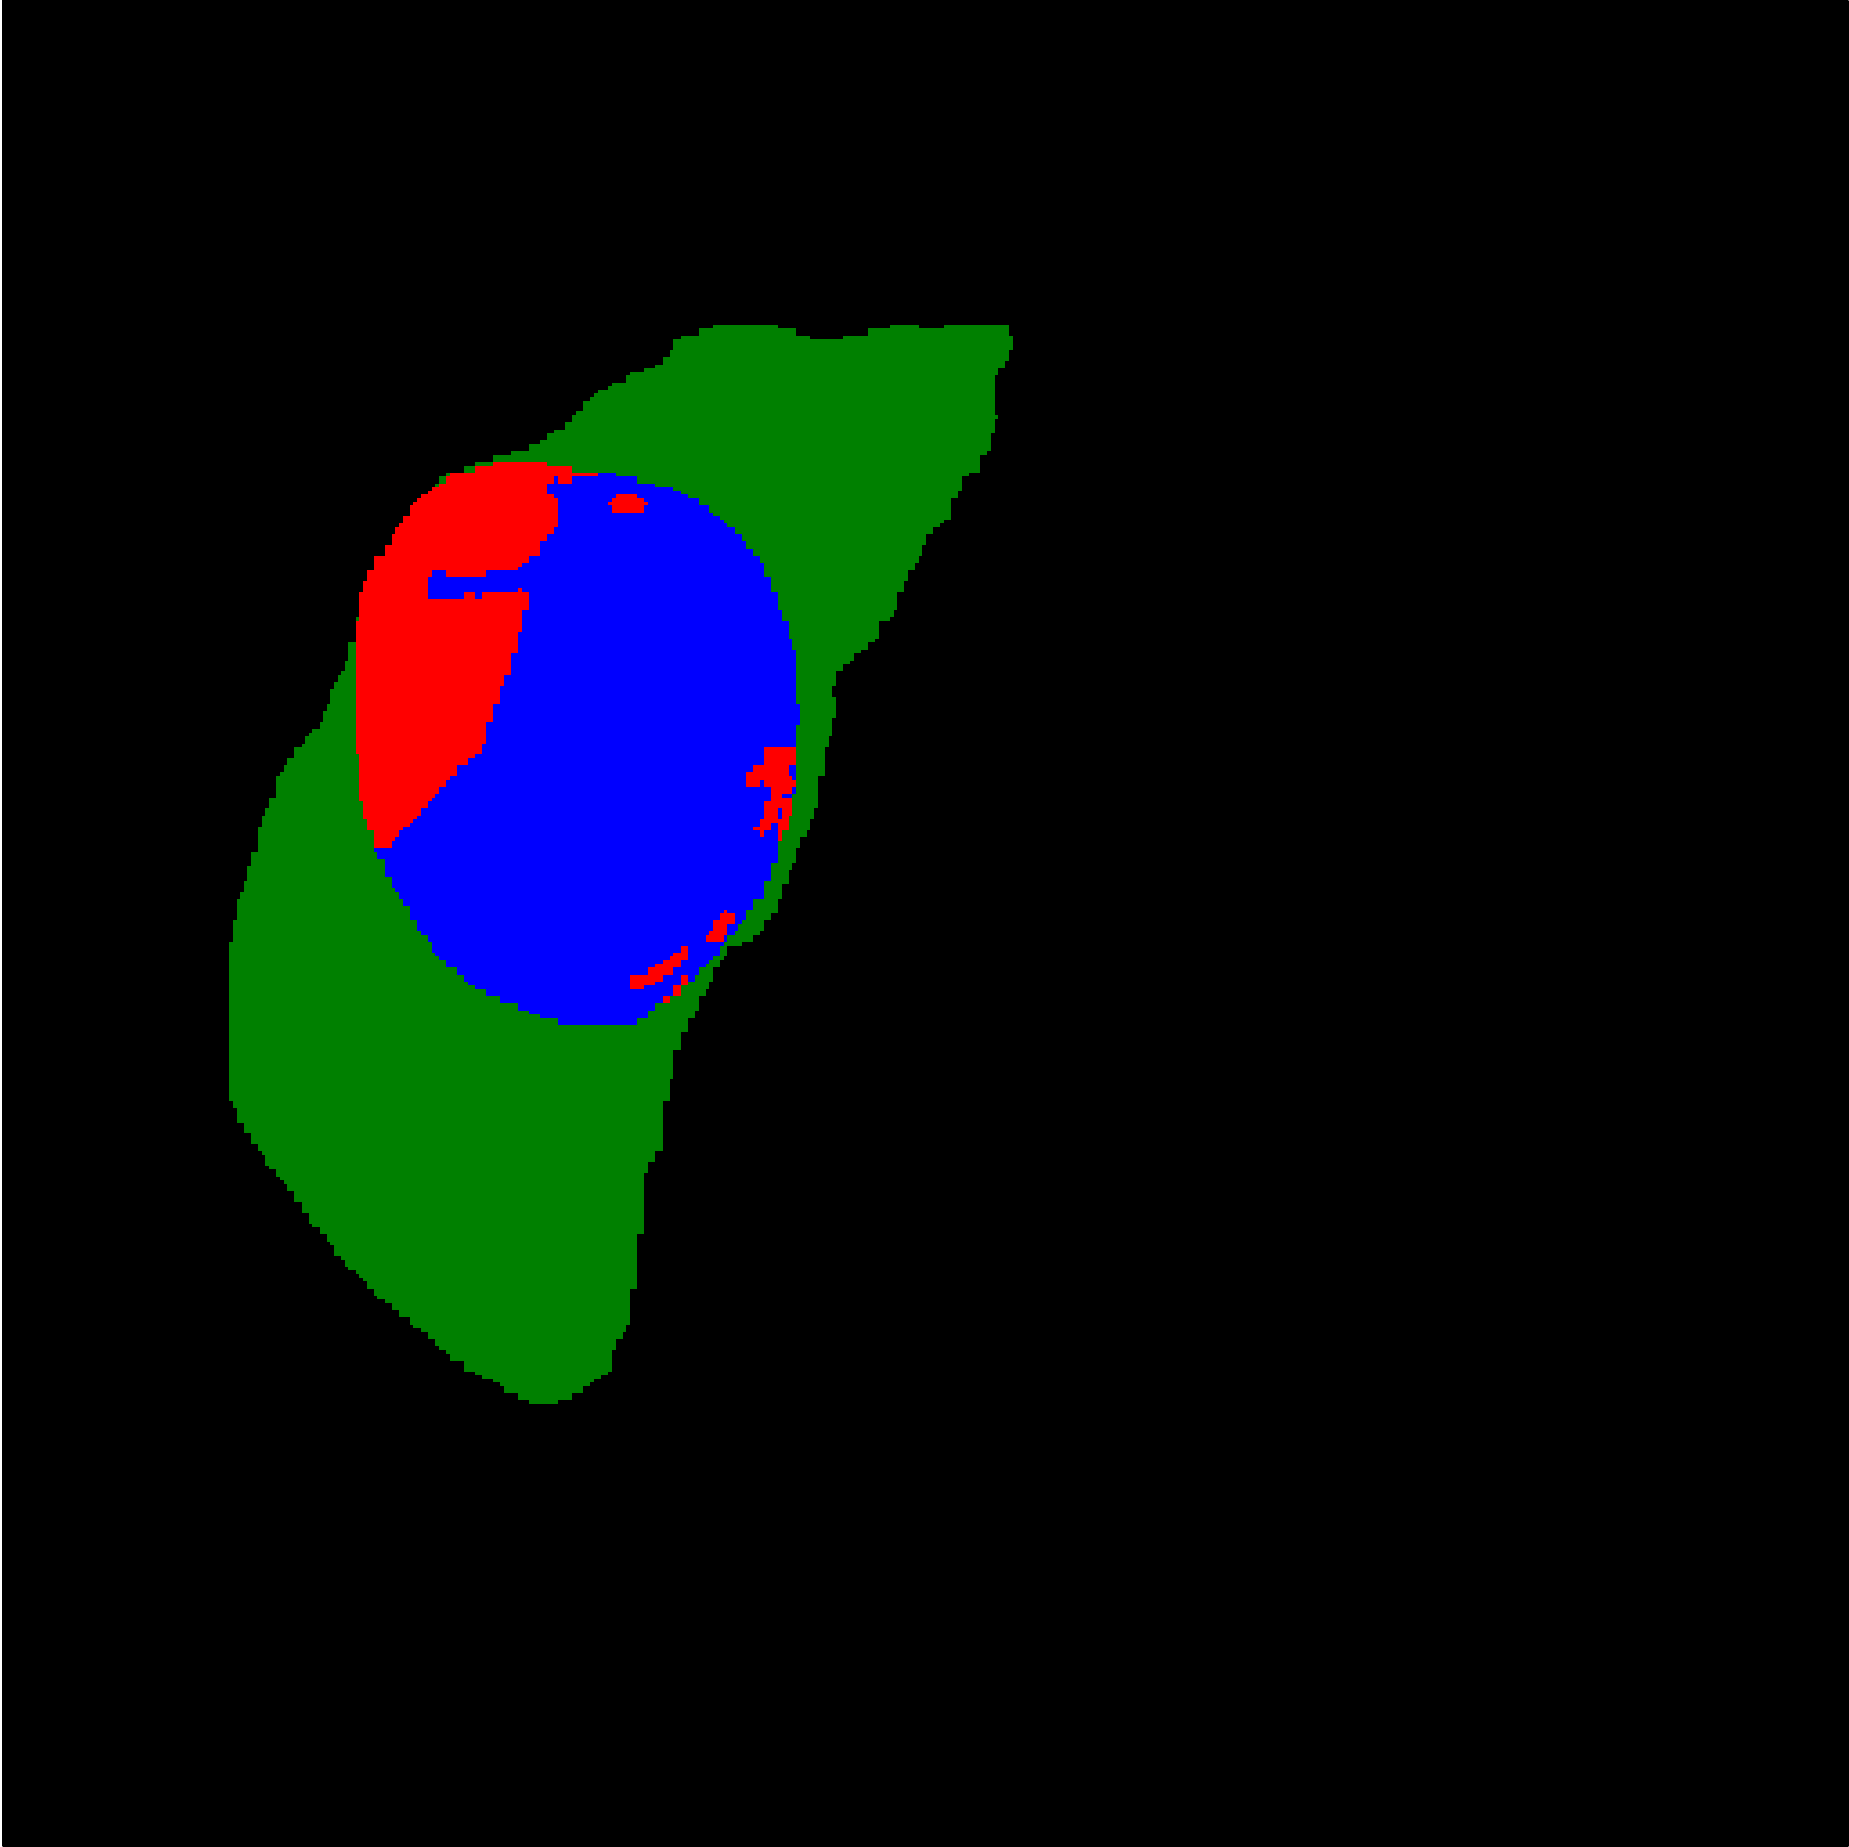
\includegraphics[width=\linewidth]{../SemanticSeg/images/1_7_gt_new_resized}
\end{minipage} \hspace{-0.3cm}
\begin{minipage}{4cm}
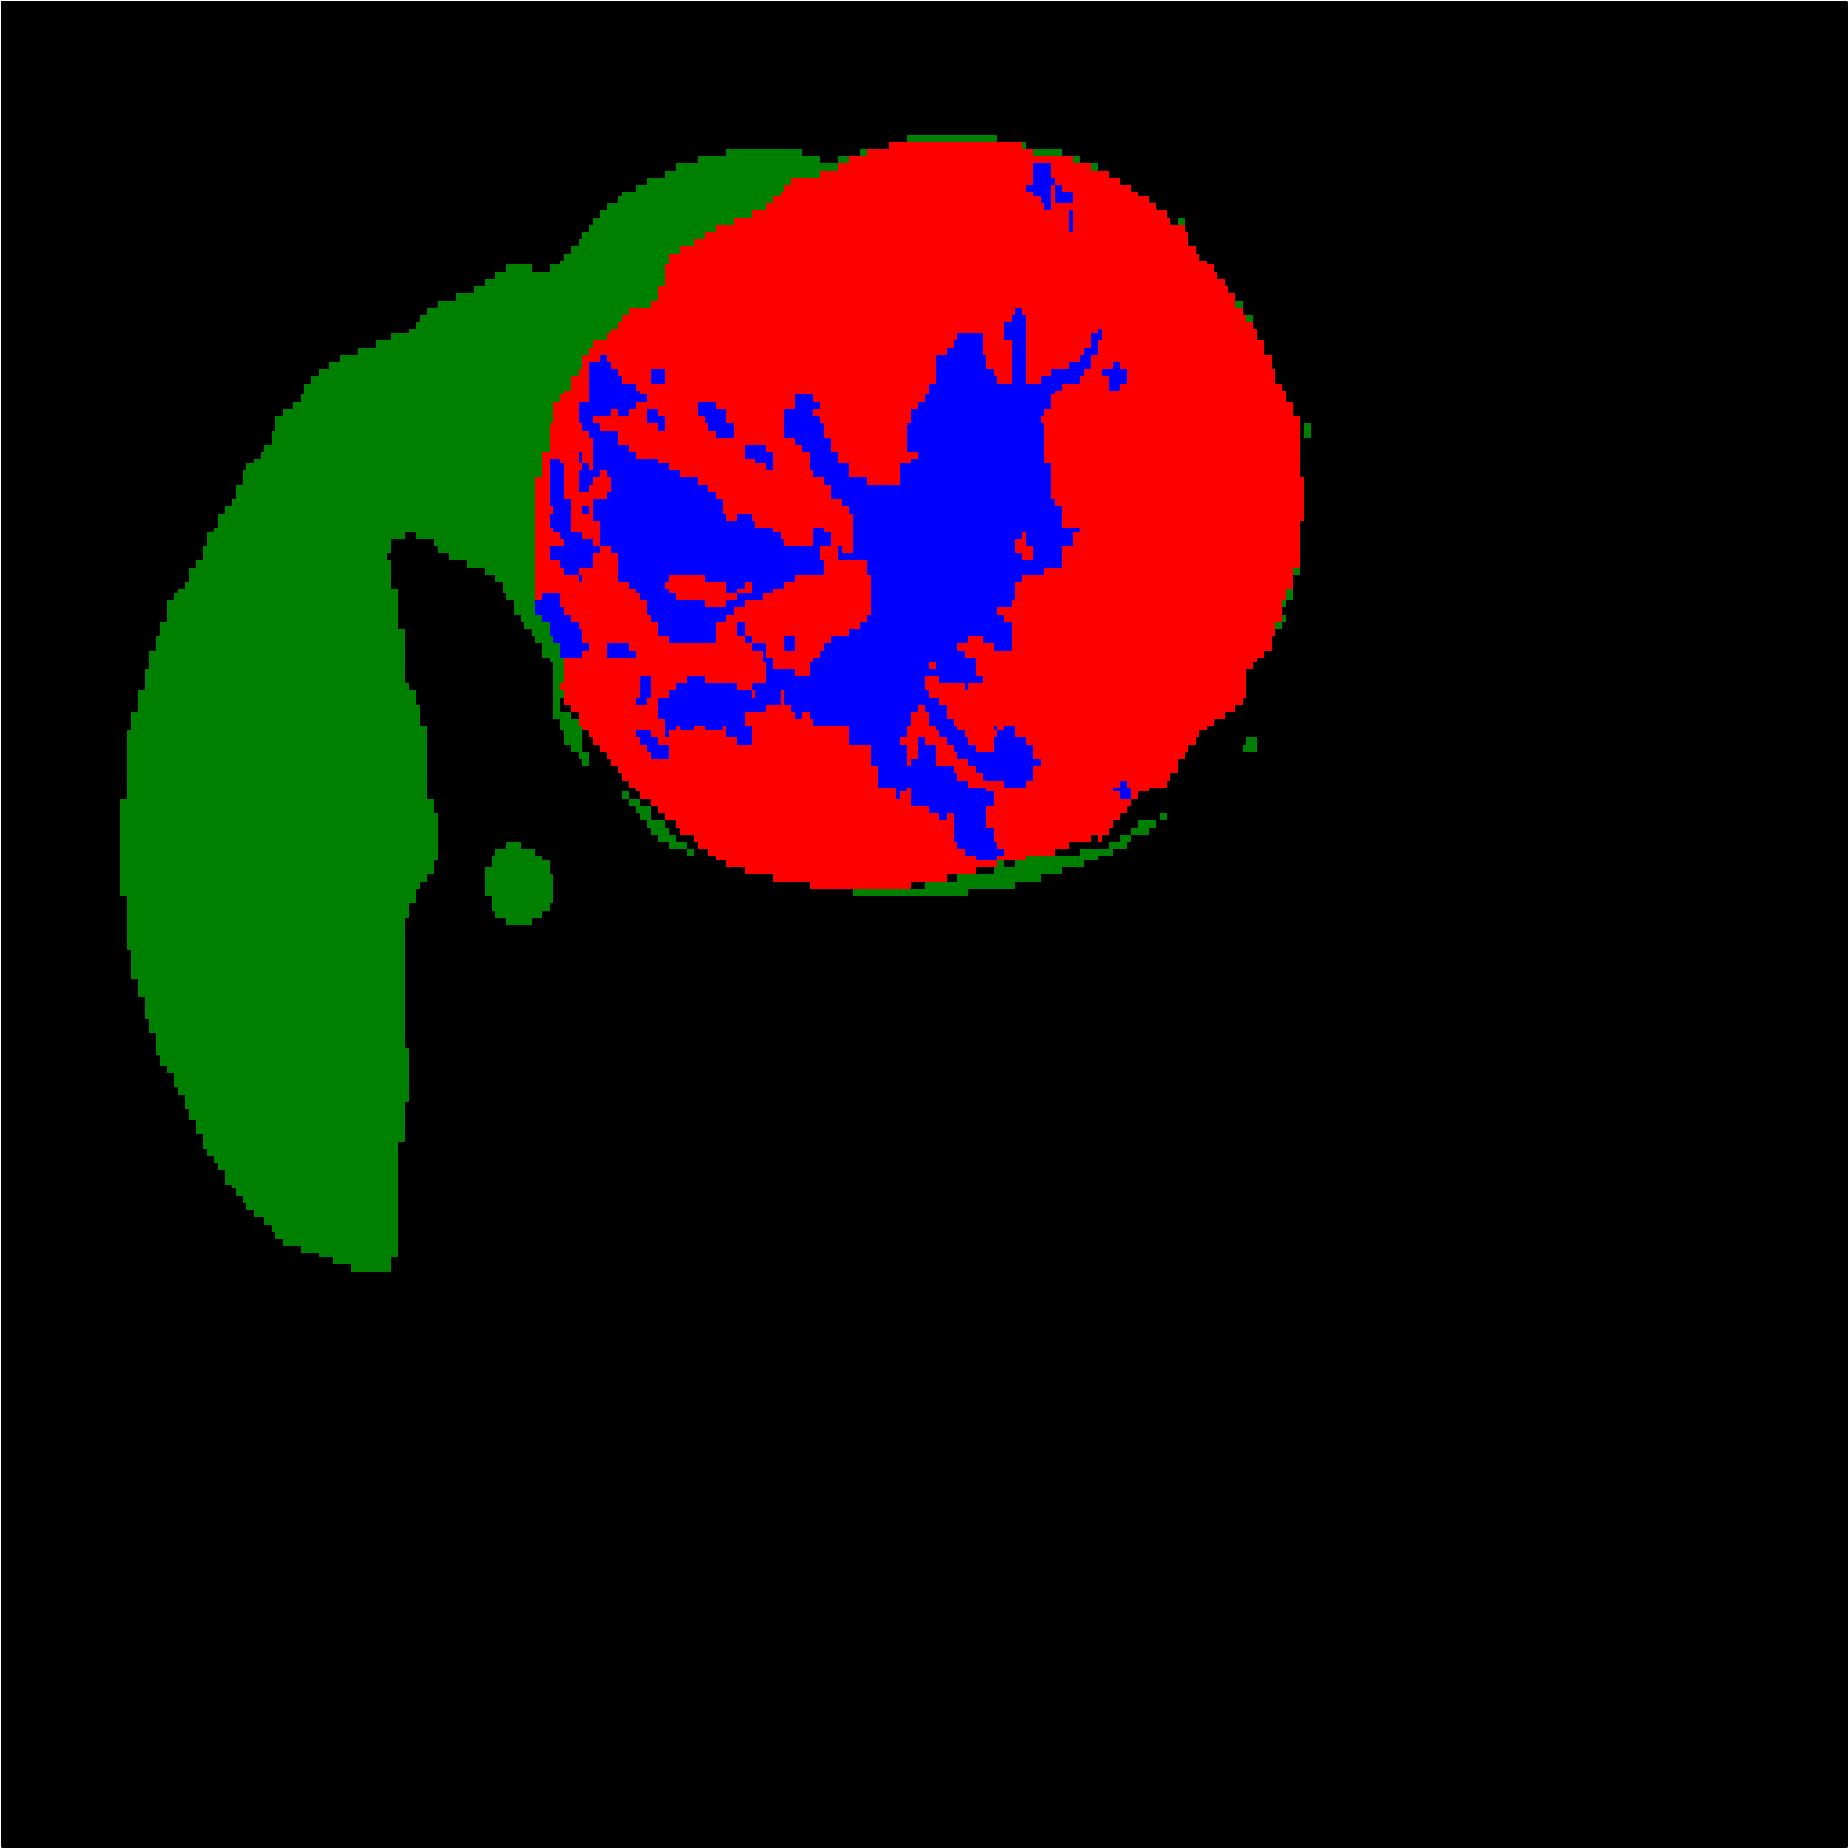
\includegraphics[width=\linewidth]{../SemanticSeg/images/2_3gt_resized}
\end{minipage} \hspace{-0.3cm}
\begin{minipage}{4cm}
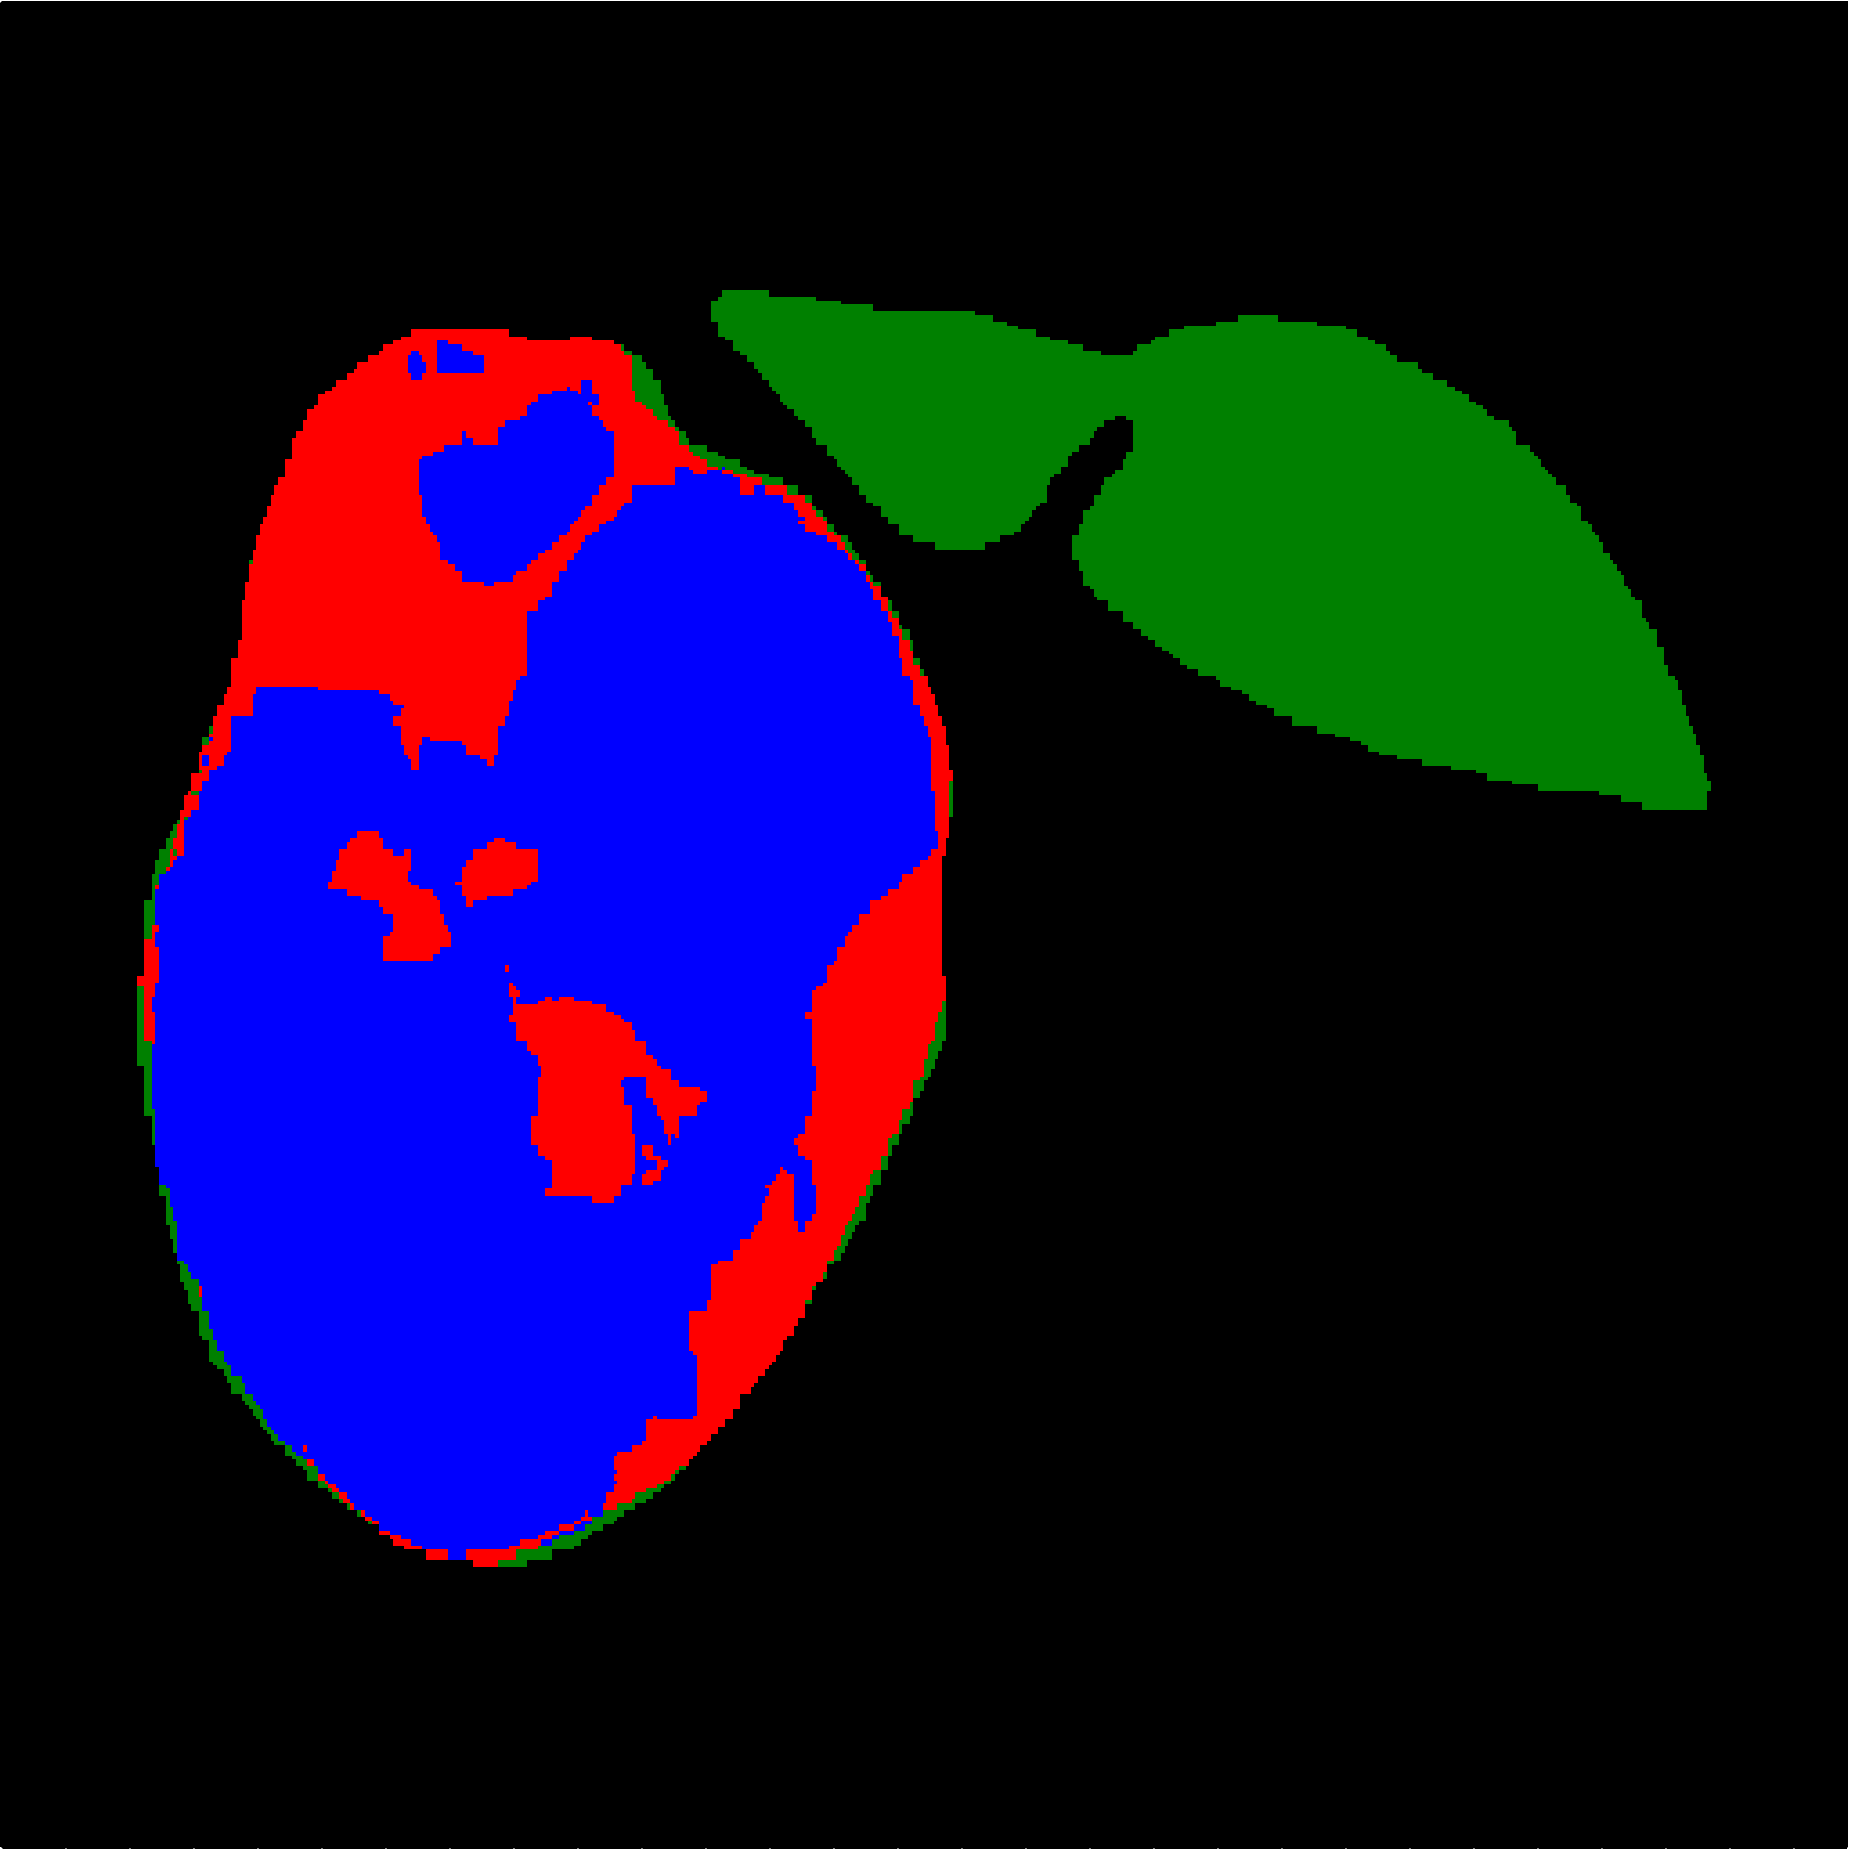
\includegraphics[width=\linewidth]{../SemanticSeg/images/5_4_gt_resized}
\end{minipage} 
\vspace{-0.2cm}
\begin{minipage}{4cm}
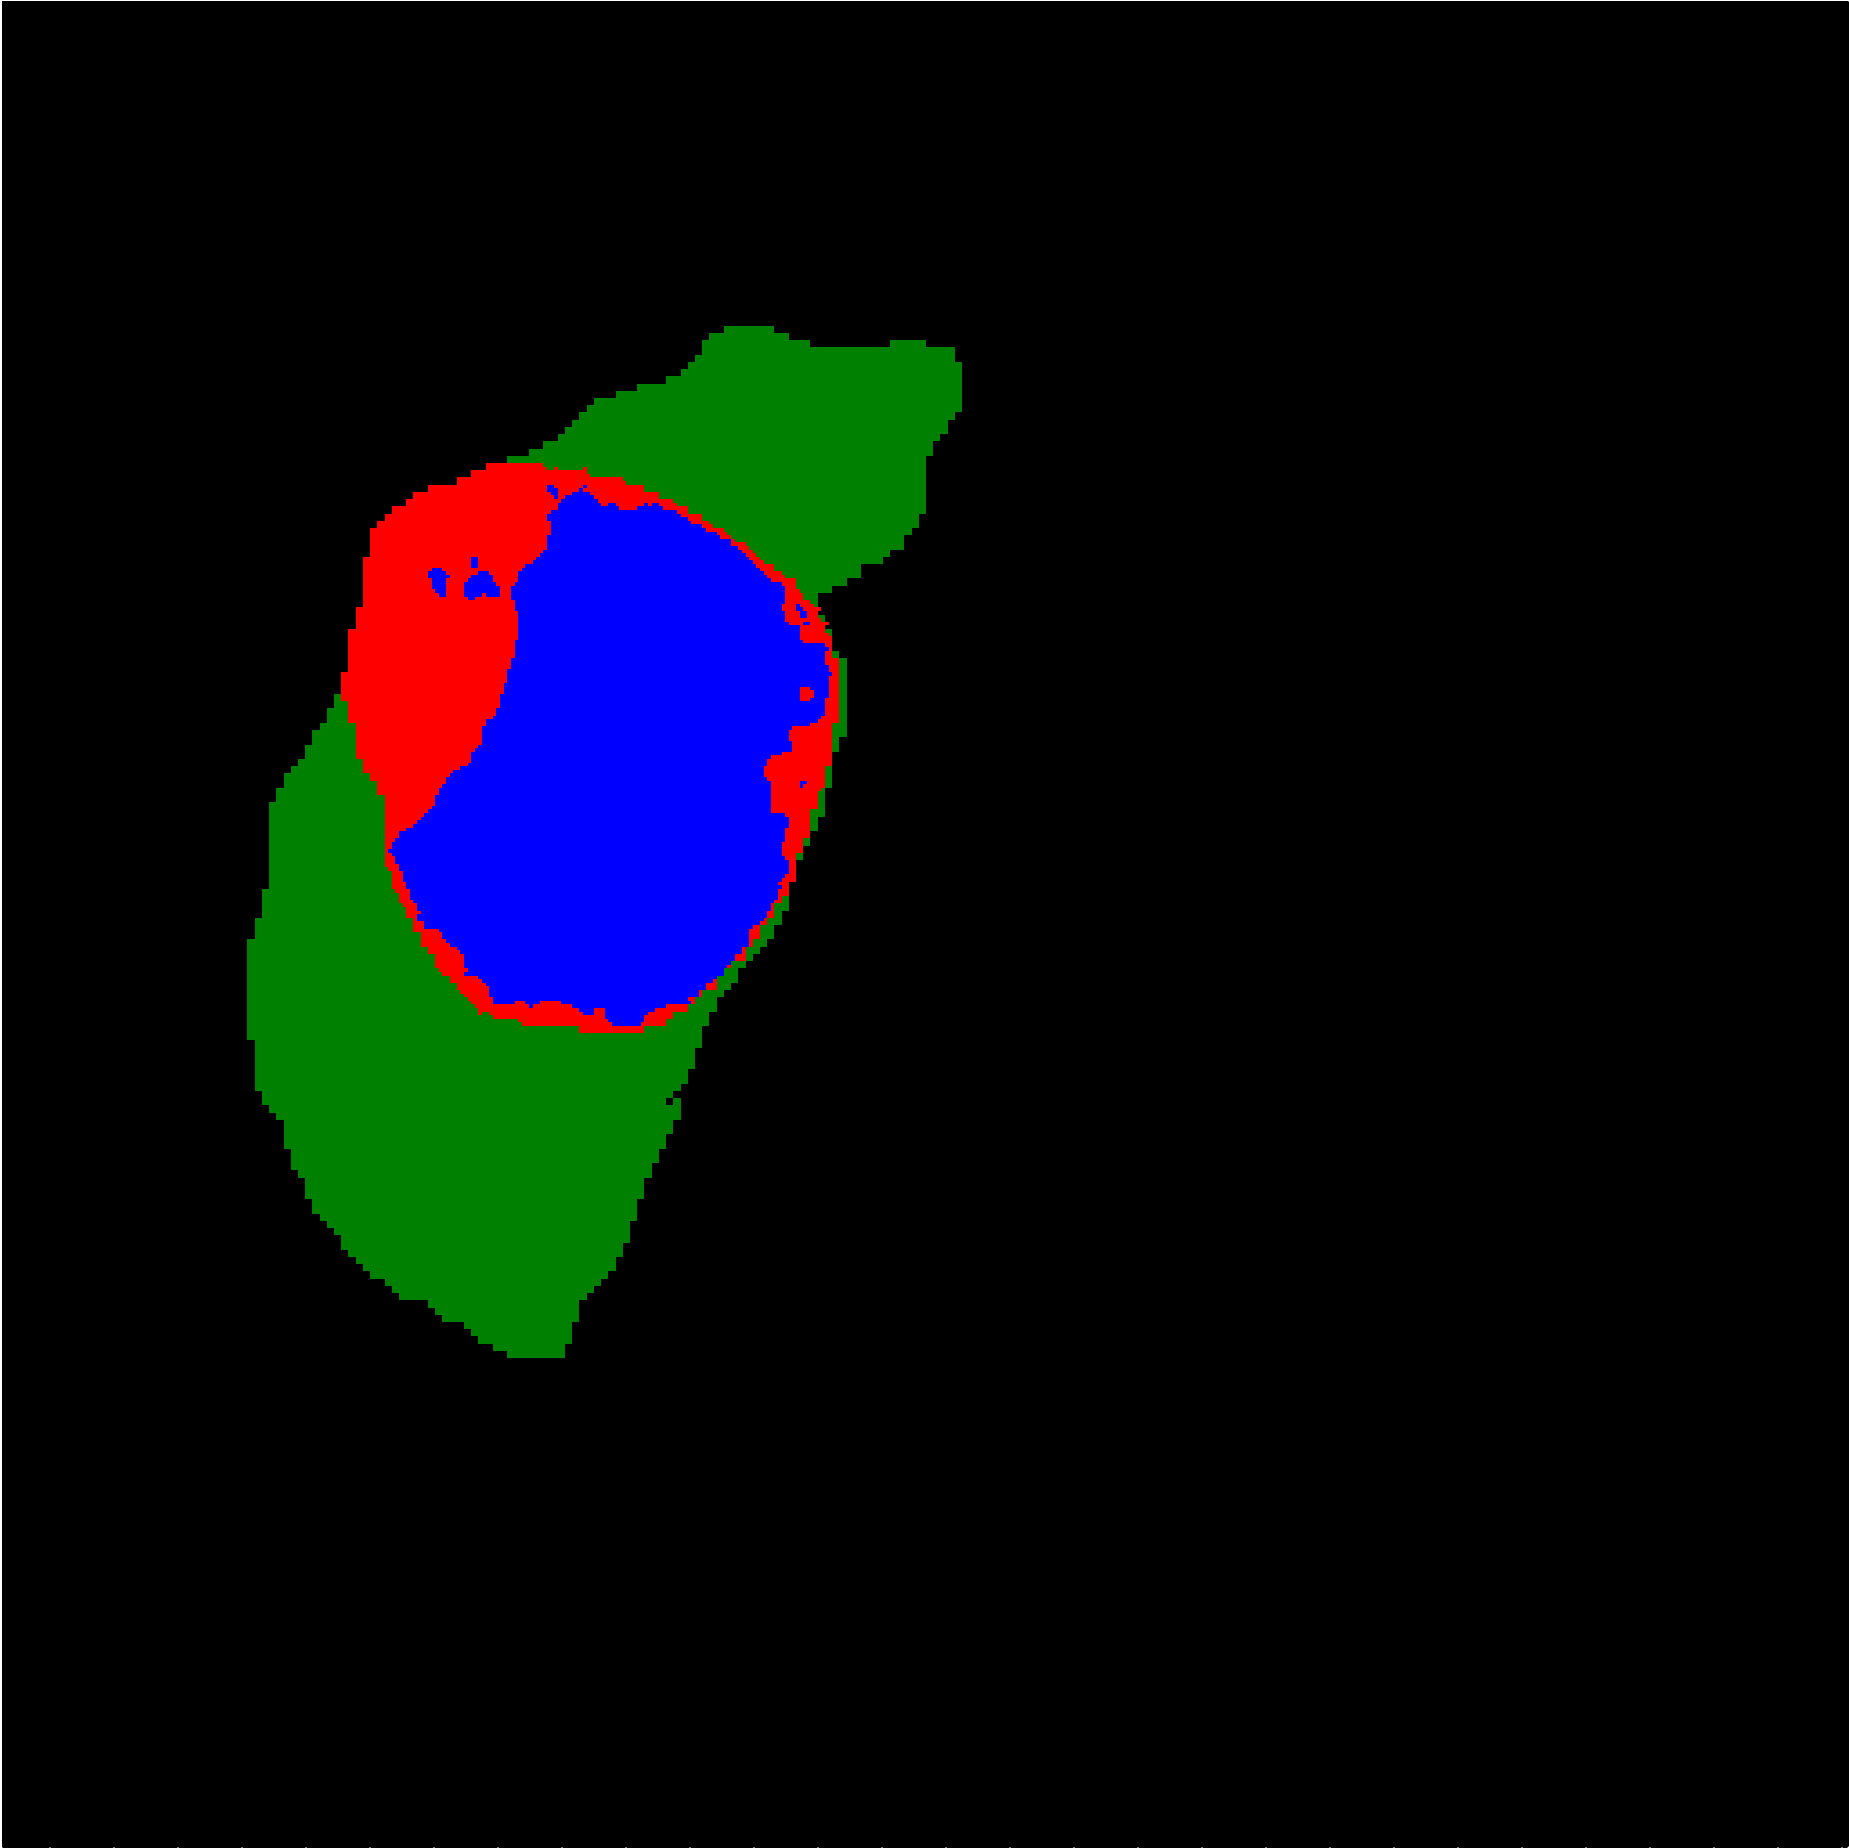
\includegraphics[width=\linewidth]{../SemanticSeg/images/1_7_FullAuto_new_resized}
\end{minipage} \hspace{-0.3cm}
\begin{minipage}{4cm}
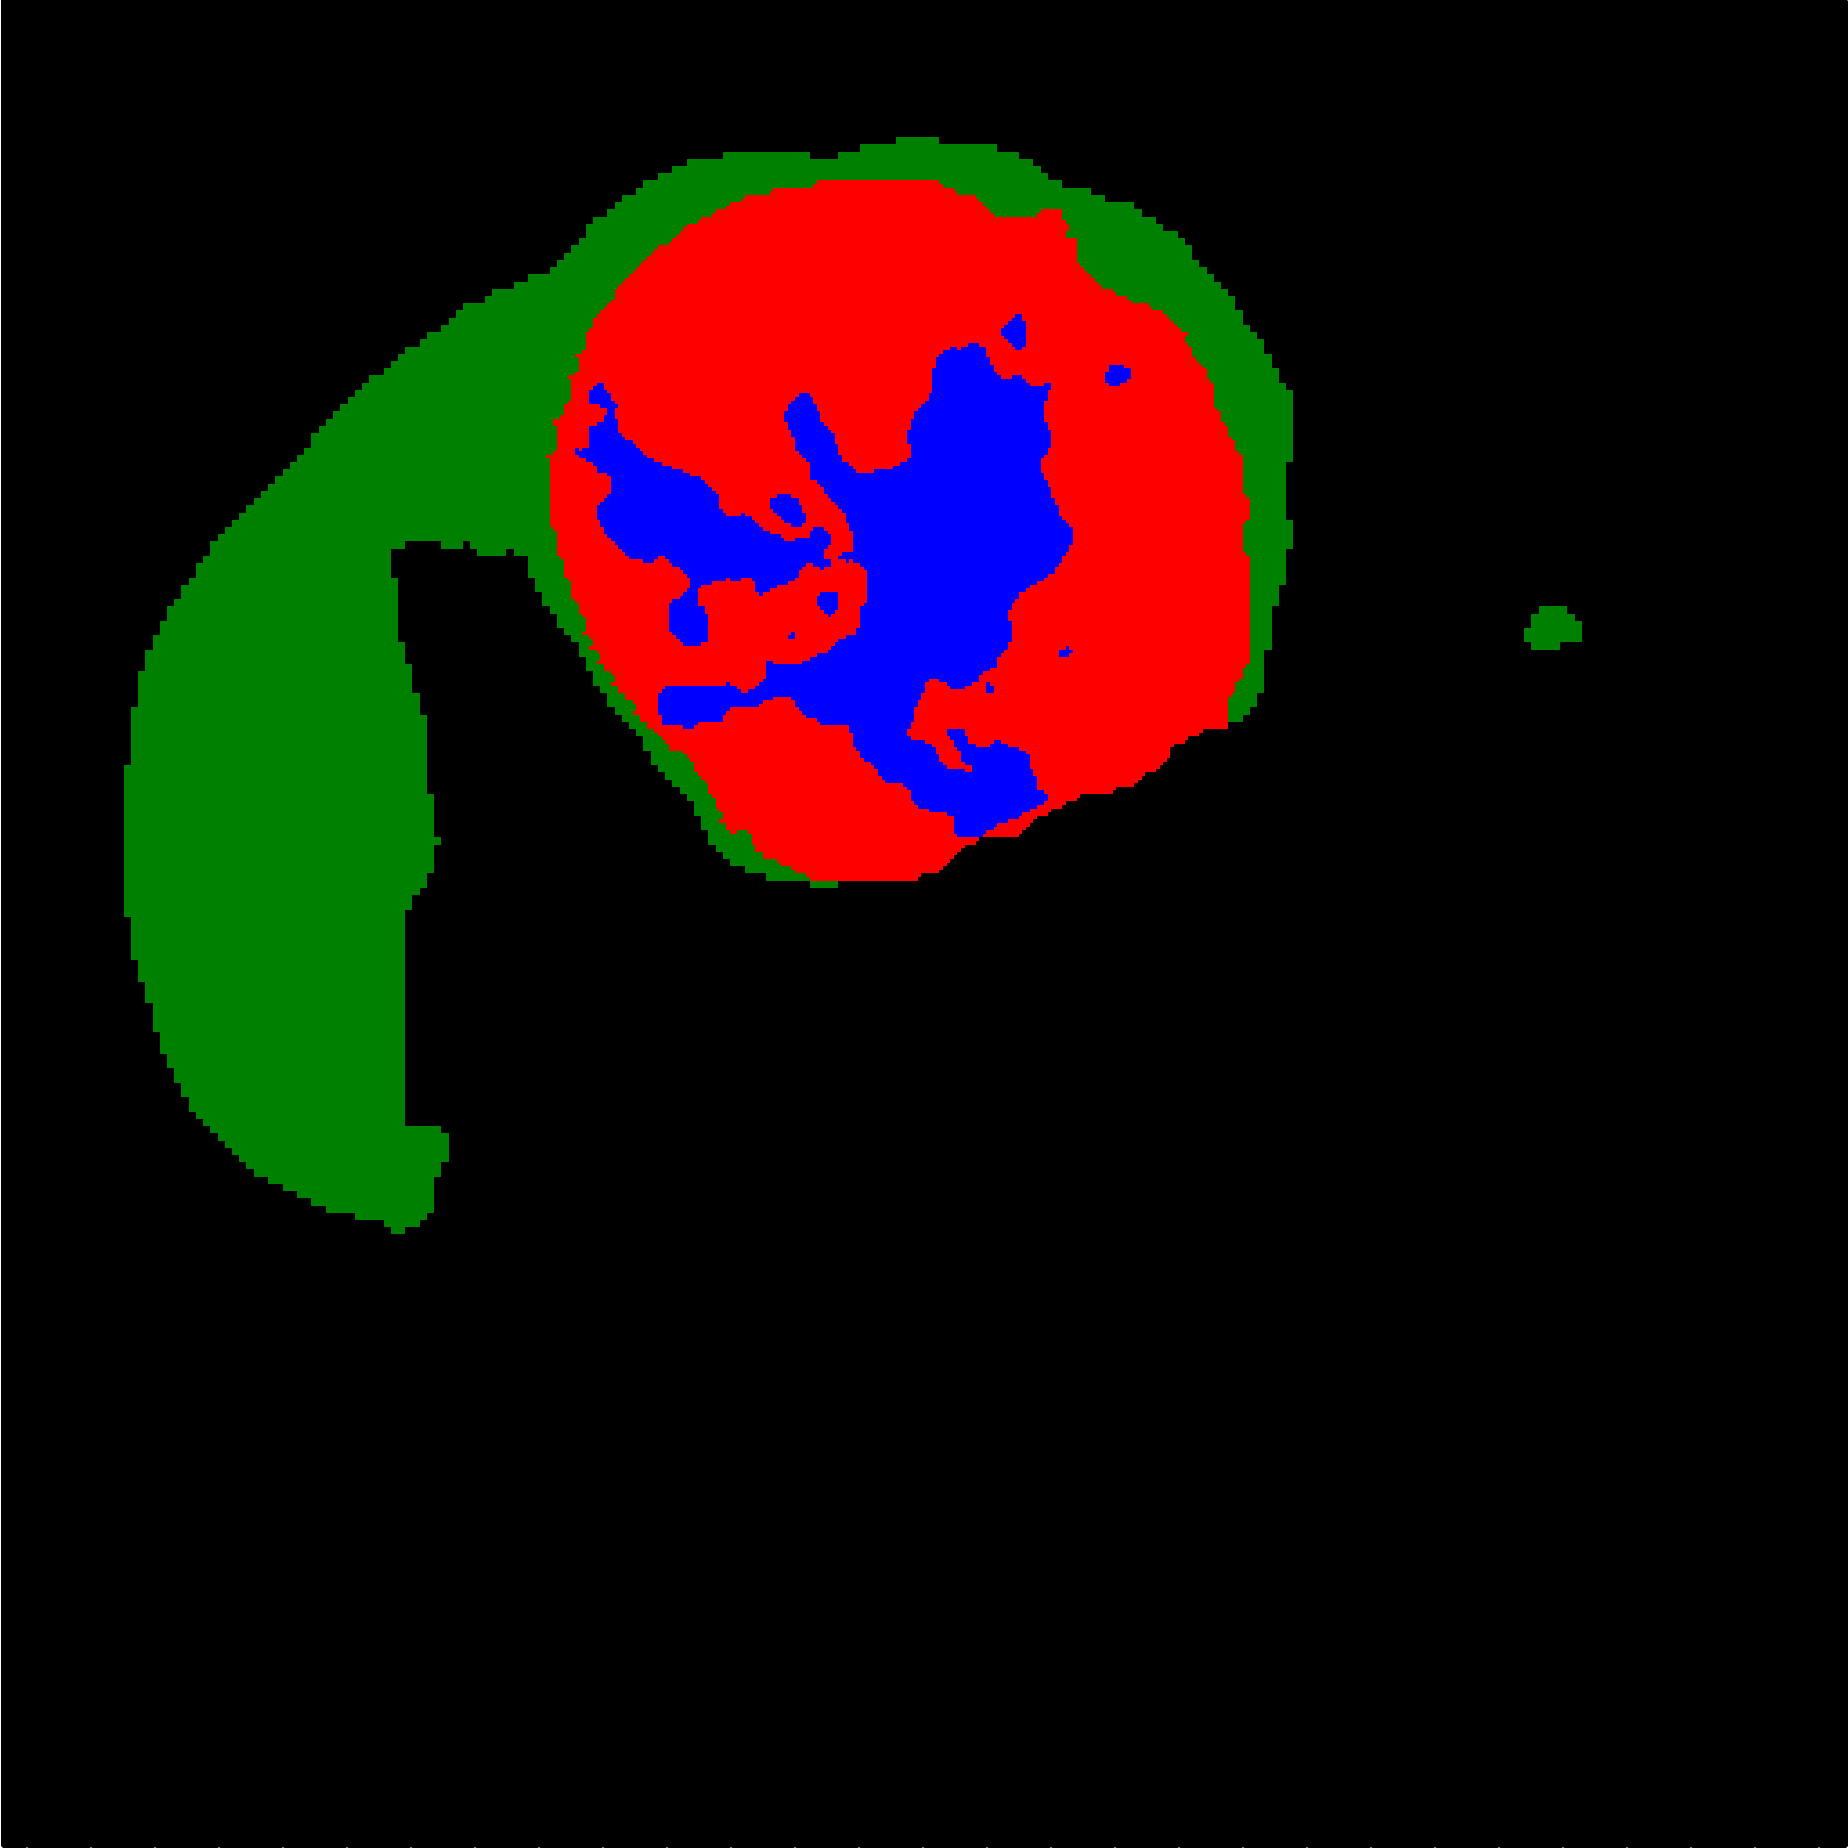
\includegraphics[width=\linewidth]{../SemanticSeg/images/2_3_FullAuto_resized}
\end{minipage} \hspace{-0.3cm}
\begin{minipage}{4cm}
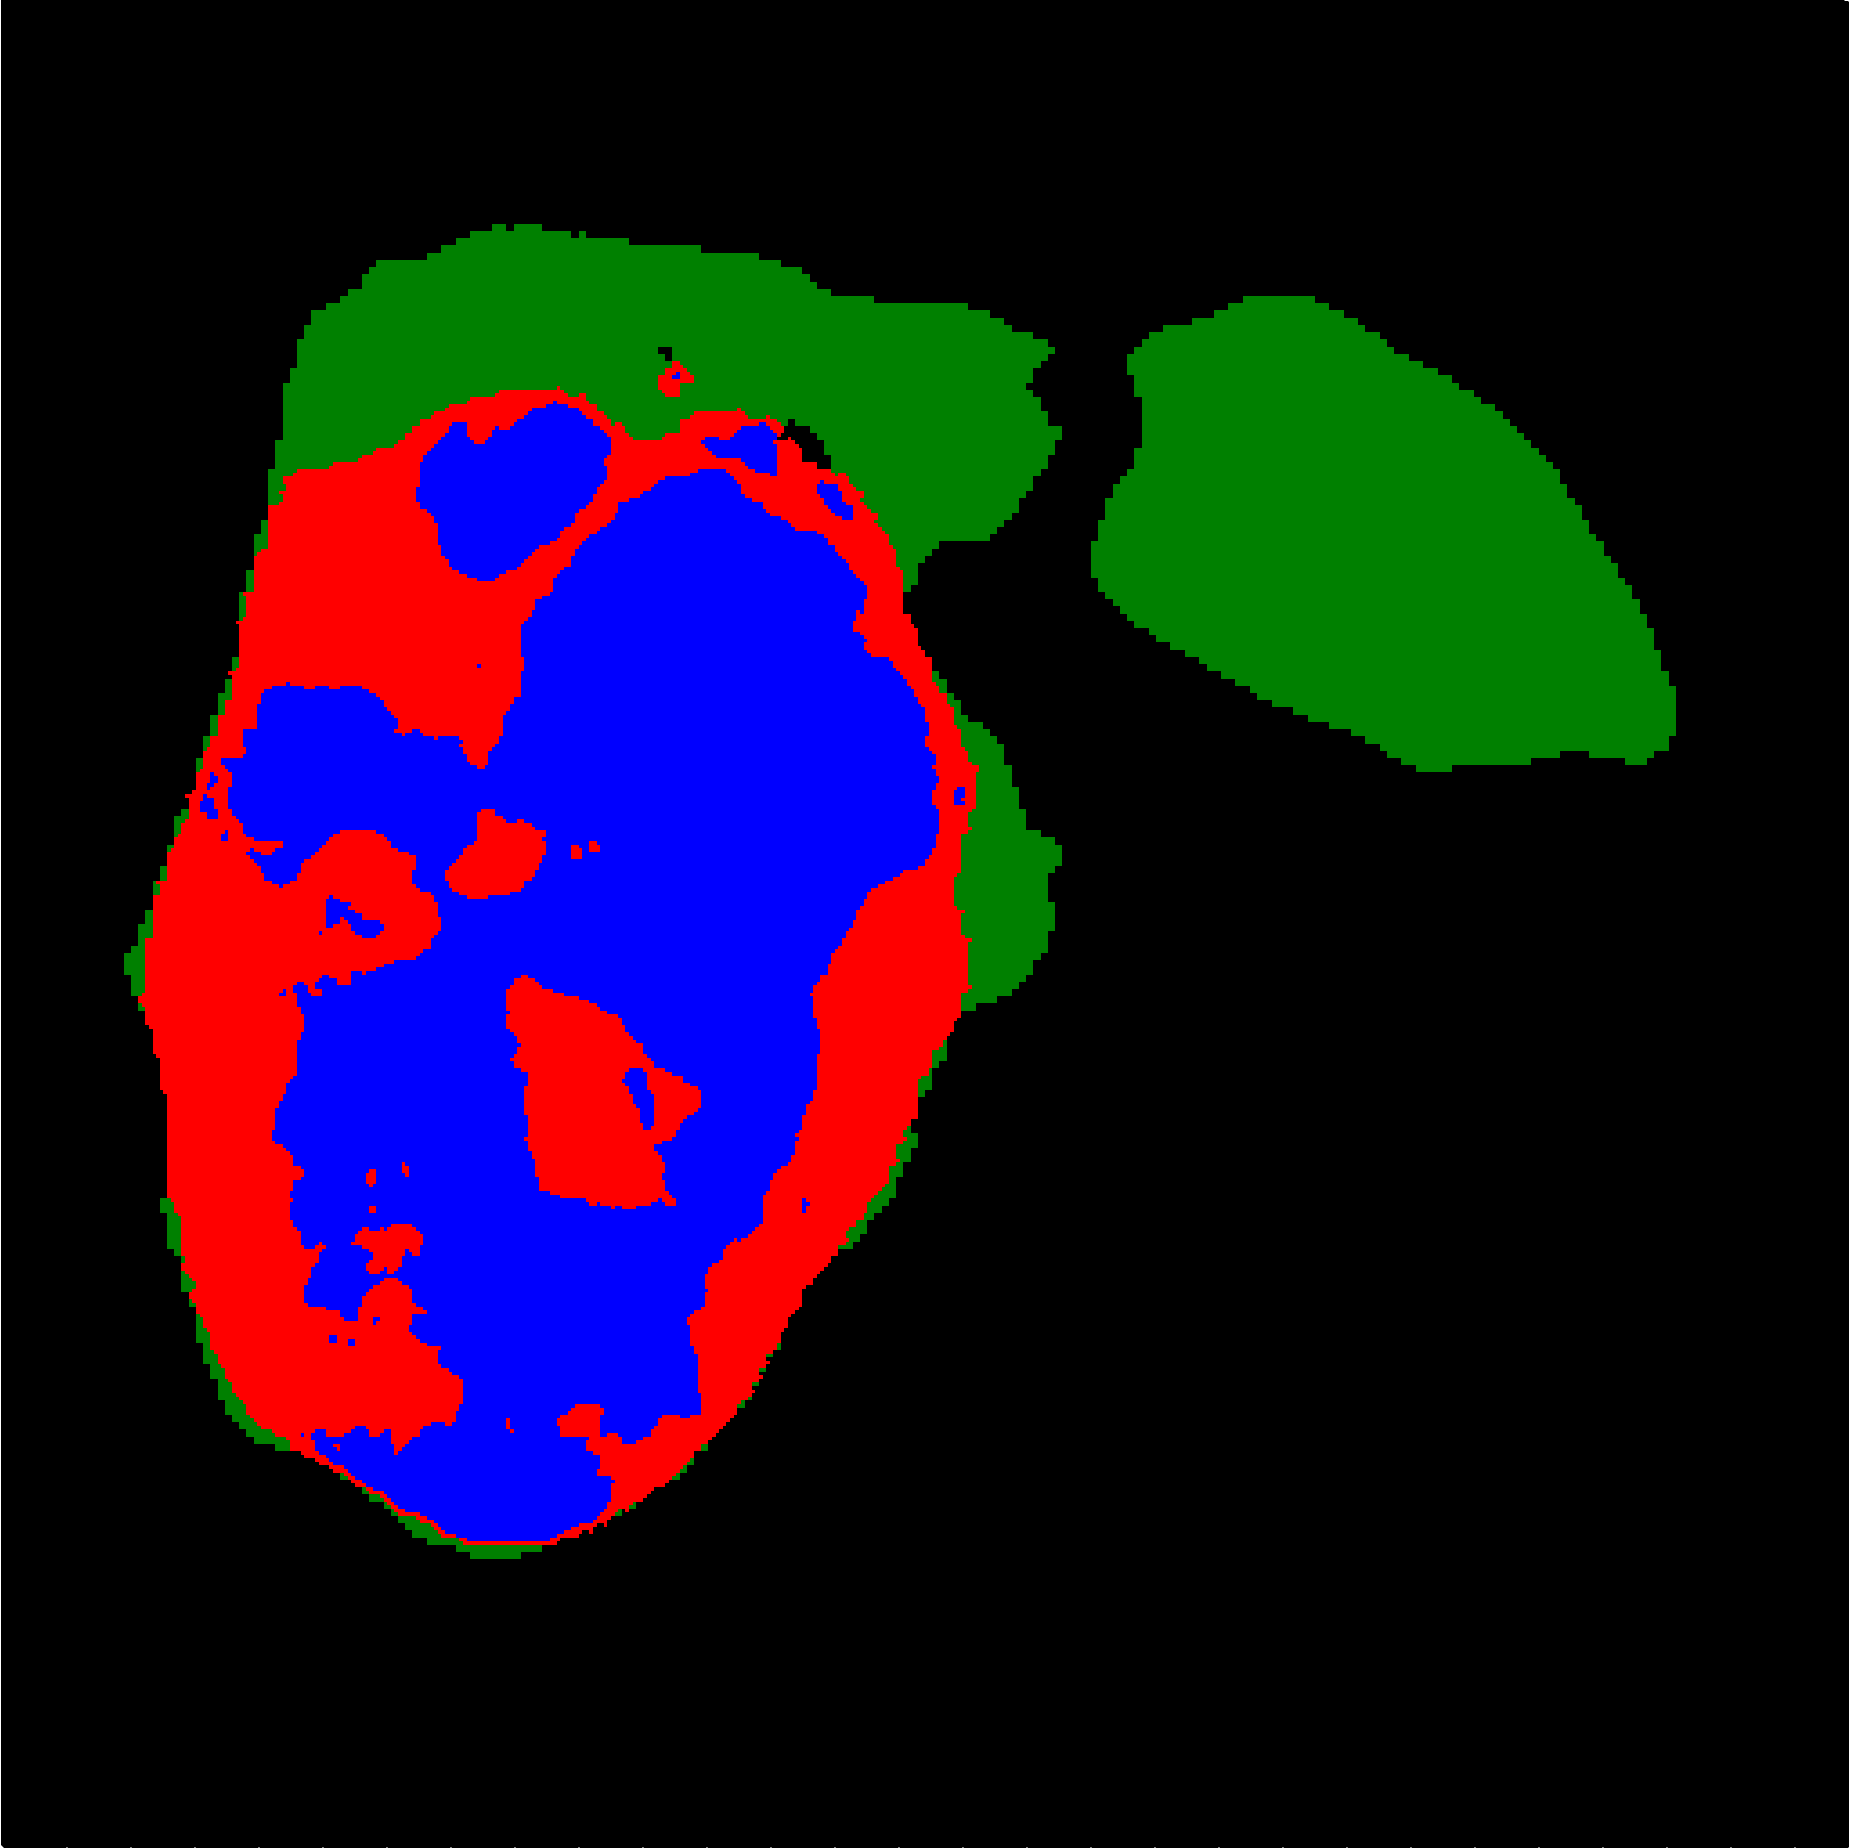
\includegraphics[width=\linewidth]{../SemanticSeg/images/5_4_FullAuto_resized}
\end{minipage} 
\caption{From top to bottom : Raw images, ground truth and results of the fully automatic segmentation of liver tissue}
\label{FullAutoSeg}
\end{figure}
\renewcommand{\baselinestretch}{1.75}
\renewcommand{\arraystretch}{5}


When comparing results obtained by the specialized networks, we proved
that the addition of the multiphase information provided better
segmentation results than when only single phase images are used.
Statistically significant improvement was obtained for the segmentation
of both the liver and the active part of the tumors.
We also investigated the performances of the single phase networks, and
noticed that the \ac{pv} phase was the one providing the best results,
where significant improvement was obtained for all the segmentation
tasks, except for the liver segmentation.
Regarding the internal liver tissues segmentation, the elementary
networks providing the best results were the \pplfont{DMP-Lesion} 
and \pplfont{DMP-Necrosis} ones. When combined in a cascaded way, 
they performed better than each one of the \pplfont{\{.\}-Full} architecture, 
with a statistically significant improvement
for the segmentation of the active part of the lesions, meaning that 
combining several specialized networks together is more efficient 
than training a single network addressing all tasks simultaneously.\\
With the same experimental conditions, our solution provided a better
accuracy for the segmentation of the lesions, and for both their active
and the necrotic parts, than the one obtained using a semi-automatic
technique with expert interaction \cite{Ouhmich2019,Conze2017}. We also
obtained equivalent results than those from a similar study considering
MR images as input \cite{Zhang2018}.\\
We concluded that the combination of multiphase registered images used in a 
cascaded architecture allows us to automatically perform the semantic segmentation of liver tissues.

